%!TEX TS-program = xelatex
%!TEX TS-options = -shell-escape
%!TEX root = ../OpAlg2_SS16/operatoralgebren2.tex
\RequirePackage{fix-cm} 
\documentclass[a4paper, twoside, headsepline, index=totoc,toc=listof,toc=bibliography,toc=index, fontsize=10pt, cleardoublepage=empty, headinclude, DIV=12, BCOR=5mm, titlepage,draft]{scrartcl}
%!TEX root = ../AnaTopGeo_SS14/ana_top_geo.tex
\usepackage{scrtime} % KOMA, Uhrzeit ermoeglicht

%--Pakete zum "Programmieren"
% ======================================================================================
\usepackage{etoolbox}
\usepackage{letltxmacro}
\usepackage{ifthen}
% ======================================================================================

%--Farbdefinitionen und Grafiken (muss vor tikz geladen werden)
% ======================================================================================
\usepackage[usenames, table, x11names]{xcolor}
\definecolor{dark_gray}{gray}{0.45}
\definecolor{light_gray}{gray}{0.6}
\definecolor{fb10_blue}{cmyk}{0.8,0.4,0.13,0.07}
\usepackage[final]{graphicx}
\usepackage{adjustbox}
\newcommand{\cfbox}[2]{% coloured frame box
	\ifmmode
	\mathchoice{\adjustbox{cfbox=#1}{$\displaystyle#2$}}{\adjustbox{cfbox=#1}{$\textstyle#2$}}{\adjustbox{cfbox=#1}{$\scriptstyle#2$}}{\adjustbox{cfbox=#1}{$\scriptscriptstyle#2$}}
	\else
	\adjustbox{cfbox=#1}{#2}
	\fi
}
% ======================================================================================

%--Zum Zeichnen/ TikZ-Kram (vor polyglossia bzw. babel geladen werden)
% ======================================================================================
\usepackage{tikz}
\usepackage{tikz-cd}
\usetikzlibrary{external}
\tikzset{>=latex}
\usetikzlibrary{%
	shapes,
	arrows.meta,
	intersections,
	calc,
	3d,
	decorations.pathreplacing,decorations.markings,decorations.pathmorphing,
	angles,
	quotes,
}
\tikzexternalize[prefix=tikz/,up to date check=diff]
\pgfkeys{/pgf/images/include external/.code=\includegraphics{#1}}
\tikzset{external/system call={lualatex \tikzexternalcheckshellescape -halt-on-error -interaction=batchmode --shell-escape -jobname "\image" "\texsource"}}
\AtBeginEnvironment{tikzcd}{\tikzexternaldisable} % tikzexternalize fuer tikzcd deaktivieren, da inkompatibel
\AtEndEnvironment{tikzcd}{\tikzexternalenable}
\tikzset{% um Inkompatibilitaeten von quotes und polyglossia bzw. babel zu vermeiden
  every picture/.append style={
    execute at begin picture={\shorthandoff{"}},
    execute at end picture={\shorthandon{"}}
  }
}
\usepackage{pgfplots}
\usepgfplotslibrary{colormaps}
\newcommand*\circled[1]{\tikzexternaldisable\tikz[baseline=(char.base)]{\node[shape=circle,draw,inner sep=2pt] (char) {#1};}\tikzexternalenable}
% ======================================================================================



%-- Mathepakete etc.
% ======================================================================================
\usepackage[T1]{fontenc}
\renewcommand{\rmdefault}{zpltlf}
\usepackage{mathtools} % beinhaltet amsmath
\mathtoolsset{showonlyrefs,centercolon,showmanualtags}
\newtagform{brackets}[\textbf]{[}{]}
\usetagform{brackets}
\usepackage{fix-cm}
\usepackage[bbgreekl]{mathbbol}
\usepackage{amssymb,marvosym} 
\usepackage{nicefrac} % schräge Brüche
\usepackage{faktor}
\newcommand{\Faktor}[1]{\faktor[\textstyle]{#1}}
\usepackage{xfrac}
\usepackage{cancel}
\usepackage{mathdots} % Verbesserung von Punkten wie zB \ldots
\usepackage[bb=px]{mathalfa} % \mathbb als px font
\usepackage{centernot}
\usepackage{stackrel}
\DeclareSymbolFont{bbold}{U}{bbold}{m}{n}
\DeclareSymbolFontAlphabet{\mathbbold}{bbold}
\newcommand{\ind}{\mathbbold{1}} % charakteristische-Funktion-Eins
\def\mathul#1#2{\color{#1}\underline{{\color{black}#2}}\color{black}} %farbiges Untersteichen im Mathe-Modus
\renewcommand{\le}{\leqslant}
\renewcommand{\ge}{\geqslant}
% ======================================================================================


%-- Von xfrac erzeuge font warnings ignorieren
% ======================================================================================
\usepackage{silence}
\WarningFilter{latexfont}{Size substitutions with differences}
\WarningFilter{latexfont}{Font shape `U/bbold/m/n' in size}
% ======================================================================================


%-- Typographie/Polyglossia
% ======================================================================================
\usepackage[euler-digits]{eulervm} % vor fontspec laden!
\usepackage[no-math]{fontspec}
\usepackage{polyglossia} % moderner babel-ersatz
\setmainlanguage[spelling=new,babelshorthands=true]{german}
\shorthandoff{"}
\setotherlanguage{english}
\defaultfontfeatures{Mapping=tex-text, WordSpace={1.2}, Ligatures={Required,Common,Contextual},Extension=.otf} %


\setmainfont{TeXGyrePagellaX}[UprightFont=*-Regular,BoldFont=*-Bold,ItalicFont=*-Italic,BoldItalicFont=*-BoldItalic,ItalicFeatures={Style=Historic},Ligatures={Required,Common,Contextual,Historic}]
\setsansfont{texgyreadventor}[Scale=MatchUppercase, UprightFont=*-regular, BoldFont=*-bold, ItalicFont=*-italic, BoldItalicFont=*-bolditalic]
\setmonofont{SourceCodePro}[Scale=0.9,UprightFont=*-Regular, BoldFont=*-Semibold, ItalicFont=*-Light]
\usepackage{xltxtra}
\usepackage{fontawesome}
\usepackage[final]{microtype}
\usepackage[draft=false]{scrlayer-scrpage} 
\flushbottom
% ======================================================================================


%-- Aufzählungen
% ======================================================================================
\usepackage[shortlabels,inline]{enumitem}
\setlist[itemize,1]{label=\faCaretRight}
\setlist[enumerate]{font=\bfseries}
\setlist[description]{font=\normalfont\bfseries}
\usepackage{multicol}
% ======================================================================================


%-- Floats/Figures/Tabellen
% ======================================================================================
\usepackage{wrapfig}
\usepackage{float}
\usepackage[margin=10pt, font=small, labelfont={sf, bf}, format=plain, indention=1em]{caption}
\captionsetup[wrapfigure]{name=Abb. }
\usepackage{booktabs}
% ======================================================================================


%-- korrekte Anführungszeichen und Zitierbefehle
% ======================================================================================
\usepackage[autostyle,german=quotes,english=british]{csquotes}
% ======================================================================================


%--Indexverarbeitung
% ======================================================================================
\usepackage{makeidx}
\newcommand{\bet}[1]{\textbf{\emph{#1}}}
\newcommand{\Index}[1]{\bet{#1}\index{#1}}
\makeindex
\setindexpreamble{{\noindent\sffamily\small Die \emph{Seitenzahlen} sind mit Hyperlinks versehen und somit anklickbar} \par \bigskip}
\renewcommand{\indexpagestyle}{scrheadings}
% ======================================================================================


%-- Marginnotes/Todonotes/Footnotes
% ======================================================================================
\deffootnote[1.5em]{1.5em}{1.5em}{\textsuperscript{\thefootnotemark}\ }
\usepackage[fulladjust]{marginnote}
\renewcommand*{\marginfont}{\itshape\footnotesize}
\usepackage[textsize=small]{todonotes}
\usepackage{ragged2e}
\renewcommand*{\raggedleftmarginnote}{\RaggedLeft}
\renewcommand*{\raggedrightmarginnote}{\RaggedRight}
\LetLtxMacro{\oldtodo}{\todo}
\renewcommand{\todo}[2][]{\tikzexternaldisable\oldtodo[#1]{#2}\tikzexternalenable}
\LetLtxMacro{\oldmissingfigure}{\missingfigure}
\renewcommand{\missingfigure}[2][]{\tikzexternaldisable\oldmissingfigure[{#1}]{#2}\tikzexternalenable}
% ======================================================================================


% -- BibLaTeX
% ======================================================================================
\usepackage[%
	backend=biber,
	sortlocale=auto,
	natbib,
	hyperref,
	backref,
	style=alphabetic
	]%
{biblatex}
\renewcommand*{\mkbibnamelast}[1]{%
  \ifmknamesc{\textsc{#1}}{#1}}
\renewcommand*{\mkbibnameprefix}[1]{%
  \ifboolexpr{ test {\ifmknamesc} and test {\ifuseprefix} }
    {\textsc{#1}}
    {#1}}
\def\ifmknamesc{%
  \ifboolexpr{ test {\ifcurrentname{labelname}}
               or test {\ifcurrentname{author}}
               or ( test {\ifnameundef{author}} and test {\ifcurrentname{editor}} ) }}
\addbibresource{../!config/quellen.bib}
% ======================================================================================

%--Konfiguration von Hyperref und Cleveref
% ======================================================================================
\usepackage[hidelinks, pdfpagelabels,  bookmarksopen=true, bookmarksnumbered=true, linkcolor=black, urlcolor=SkyBlue2, plainpages=false,pagebackref, citecolor=black, hypertexnames=true, pdfauthor={Jannes Bantje}, pdfborderstyle={/S/U}, linkbordercolor=SkyBlue2, colorlinks=false,final,backref=false]{hyperref}
\usepackage[nameinlink,noabbrev]{cleveref}
\newcommand{\appendLink}[1]{#1\,\faExternalLink}
\newcommand{\hrefsym}[2]{\href{#1}{\texttt{\appendLink{#2}}}}
\newcommand{\hrefsymX}[2]{\href{#1}{\appendLink{#2}}}
\newcommand{\hrefsymmail}[2]{\href{#1}{\texttt{\faEnvelopeO\,#2}}}
\renewcommand{\url}[1]{\hrefsym{#1}{\nolinkurl{#1}}}
% ======================================================================================


% -- QR-Codes (hinter hyperref laden!)
% ======================================================================================
\usepackage{qrcode}
% ======================================================================================

%--Römische Zahlen
% ======================================================================================
\newcommand{\RM}[1]{\MakeUppercase{\romannumeral #1{}}}
% ======================================================================================

%-- Definition von diversen Mathe-Befehlen
% ======================================================================================
%!TEX root = mitschrift_main.tex

% -- Zum Finetuning von Befehlen
% ======================================================================================
\makeatletter
\newcommand{\raisemath}[1]{\mathpalette{\raisem@th{#1}}}
\newcommand{\raisem@th}[3]{\raisebox{#1}{$#2#3$}}
\makeatother
\makeatletter
\newcommand{\killDescendersM}[1]{\mathpalette{\killD@scendersM{#1}}}
\newcommand{\killD@scendersM}[2]{\raisebox{0pt}[\height][0pt]{$#2#1$}}
\makeatother
\DeclareRobustCommand{\minwidthbox}[2]{%
  \ifmmode
    \expandafter\mathmakebox
  \else
    \expandafter\makebox
  \fi
  [\ifdim#2<\width\width\else#2\fi]{#1}%
}
% ======================================================================================


%-- Klammerbefehle
% ======================================================================================
\DeclarePairedDelimiter{\abs}{\lvert}{\rvert}
\DeclarePairedDelimiter{\floor}{\lfloor}{\rfloor}
\DeclarePairedDelimiter{\ceil}{\lceil}{\rceil}
\DeclarePairedDelimiter\norm{\Vert}{\Vert}
\DeclarePairedDelimiter\enbrace{(}{)}
\DeclarePairedDelimiter\benbrace{[}{]}
\DeclarePairedDelimiter\bbenbrace{[\![}{]\!]}
\DeclarePairedDelimiter\lenbrace{<}{>}
\DeclarePairedDelimiter\angbrace{\langle}{\rangle}
\newcommand{\ssbrace}[1]{{\scriptscriptstyle\enbrace{#1}}}
\newcommand{\ssbbrace}[1]{{\scriptscriptstyle\benbrace{#1}}}
% ======================================================================================

%-- Mengen
% ======================================================================================
\newcommand\SetSymbol[1][]{\nonscript\:#1\vert\allowbreak\nonscript\:\mathopen{}}
\providecommand\given{} % to make it exist
\DeclarePairedDelimiterX\set[1]\{\}{\renewcommand\given{\SetSymbol[\delimsize]}#1}
% ======================================================================================

%-- Skalarprodukt (3 Varianten) 
% ======================================================================================
\DeclarePairedDelimiterX\sprod[2]{\langle}{\rangle}{#1\,\delimsize\vert\,#2}
\DeclarePairedDelimiterX\skal[2]{\langle}{\rangle}{#1\,,\,#2}
\makeatletter
\DeclareFontFamily{OMX}{MnSymbolE}{}
\DeclareSymbolFont{MnLargeSymbols}{OMX}{MnSymbolE}{m}{n}
\SetSymbolFont{MnLargeSymbols}{bold}{OMX}{MnSymbolE}{b}{n}
\DeclareFontShape{OMX}{MnSymbolE}{m}{n}{
    <-6>  MnSymbolE5
   <6-7>  MnSymbolE6
   <7-8>  MnSymbolE7
   <8-9>  MnSymbolE8
   <9-10> MnSymbolE9
  <10-12> MnSymbolE10
  <12->   MnSymbolE12
}{}
\DeclareFontShape{OMX}{MnSymbolE}{b}{n}{
    <-6>  MnSymbolE-Bold5
   <6-7>  MnSymbolE-Bold6
   <7-8>  MnSymbolE-Bold7
   <8-9>  MnSymbolE-Bold8
   <9-10> MnSymbolE-Bold9
  <10-12> MnSymbolE-Bold10
  <12->   MnSymbolE-Bold12
}{}
\let\llangle\@undefined
\let\rrangle\@undefined
\DeclareMathDelimiter{\llangle}{\mathopen}%
                     {MnLargeSymbols}{'164}{MnLargeSymbols}{'164}
\DeclareMathDelimiter{\rrangle}{\mathclose}%
                     {MnLargeSymbols}{'171}{MnLargeSymbols}{'171}
\makeatother
\DeclarePairedDelimiterX\sskal[2]{\llangle}{\rrangle}{#1\,,\,#2}
% ======================================================================================

%-- Abbildungsdefinition
% ======================================================================================
\newcommand{\mapdef}[5]{%
	\[
		\begin{array}{rcl}
			\textstyle #1 &\xrightarrow{\minwidthbox{#5}{2em}} & \textstyle #2 \\[0.5ex]
			\textstyle #3 &\xmapsto{\minwidthbox{\mbox{ }}{2em}} & \textstyle #4
		\end{array}
	\]
}
% ======================================================================================

%-- modifiziertes Stackrel 
% ======================================================================================
\newcommand{\StackText}[2]{\stackrel{\mbox{\scriptsize #1}}{#2}}
\newcommand{\StackTextClap}[2]{\stackrel{\mathclap{\mbox{\scriptsize #1}}}{#2}}
% ======================================================================================

%-- Blitz
% ======================================================================================
\newcommand{\light}{\text{\raisebox{-.3ex}{\Large\Lightning}}}
% ======================================================================================


%-- Underbrace u.Ä. als Befehl in LaTeX-Syntax (und ohne Spacingprobleme mit nachfolgenden Operatoren...)
% ======================================================================================
\newcommand{\Underbrace}[2]{{\underbrace{#1}_{#2}}}
\newcommand{\Underbracket}[2]{{\underbracket[0.7pt][2pt]{#1}_{#2}}}
\newcommand{\Overbracket}[2]{{\overbracket[0.7pt][2pt]{#1}^{#2}}}
% ======================================================================================


%-- Deklaration weiterer Operatoren (allgemein)
% ======================================================================================
\DeclareMathOperator{\re}{Re} % Realteil
\let\Re\relax
\DeclareMathOperator{\Re}{Re} % Realteil
\DeclareMathOperator{\im}{im} % Bild
\let\Im\relax
\DeclareMathOperator{\Im}{Im} % Bild
\DeclareMathOperator{\id}{id} % identische Abbildung
\DeclareMathOperator{\conj}{conj} % Konjugation
\DeclareMathOperator{\sgn}{sgn} % Signum
\DeclareMathOperator{\End}{End} % Endomorphismen
\DeclareMathOperator{\Hom}{Hom} % Homomorphismen
\DeclareMathOperator{\Iso}{Iso} % Isomorphismen
\DeclareMathOperator{\Aut}{Aut} % Automorphismen
\DeclareMathOperator{\Span}{span} % Span
\DeclareMathOperator{\coker}{coker} % Kokern
\DeclareMathOperator{\Tr}{Tr} % Spur,Trace
\DeclareMathOperator{\pr}{pr} % Projektion
\DeclareMathOperator{\diag}{diag} % Diagonalmatrix
\DeclareMathOperator{\Rg}{Rg} % Rang
\DeclareMathOperator{\const}{const} % konstante Abbildung
\DeclareMathOperator{\Spur}{Spur} % Spur
\DeclareMathOperator{\Arg}{Arg} % Argument
\DeclareMathOperator{\dist}{dist} % Distanz
\DeclareMathOperator{\supp}{supp} % Träger
\DeclareMathOperator{\Char}{char} % Charakteristik
% ======================================================================================


%-- Deklaration weiterer Operatoren (Differentiale etc.)
% ======================================================================================
\DeclareMathOperator{\grad}{grad} % Gradient
\DeclareMathOperator{\dive}{div} % Gradient
\DeclareMathOperator{\rot}{rot} % Rotation
\newcommand{\D}{\ensuremath{\mathrm{D}\mkern-1.0mu}} % Differential
\newcommand{\mathd}{\ensuremath{\mathrm{d}\mkern-1.0mu}} % äußere Ableitung
\newcommand{\Tmap}{\ensuremath{\mathrm{T}\mkern-0.85mu}} % Tangentialraum
\let\Tang\Tmap
\DeclareMathOperator{\Diff}{Diff}
\newcommand{\diff}[2]{\ensuremath{\frac{{\partial #1}}{{\partial #2}} }}
\newcommand{\diffd}[2]{\ensuremath{\frac{\mathd #1}{\mathd #2} }}
% ======================================================================================


%-- Deklaration weiterer Operatoren (Topologie)
% ======================================================================================
\newcommand*\interior[1]{\overset{\smash{\raisebox{-0.18ex}{$\scriptstyle\circ$}}}{#1}}
\newcommand{\sing}{{\raisemath{1.1pt}{\scriptscriptstyle\mathrm{sing}}}}
\newcommand{\pt}{\mathrm{pt}}
\DeclareMathOperator{\Zyl}{Zyl}
\DeclareMathOperator{\Tel}{Tel}
\newcommand{\op}{\mathrm{op}}
\DeclareMathOperator{\Sp}{Sp}
\DeclareMathOperator{\Keg}{Keg}
\newcommand{\slashedi}{i\hspace{-3.5pt}/}
\newcommand{\cupp}{\smallsmile}
\newcommand{\capp}{\smallfrown}
\DeclareMathOperator*{\colim}{colim}
\DeclareMathOperator{\PD}{PD}
\newcommand{\lf}{\mathrm{lf}}
\DeclareMathOperator{\sig}{sig}
\DeclareMathOperator{\Tor}{Tor}
\DeclareMathOperator{\Ext}{Ext}
\DeclareMathOperator{\AW}{AW}
\DeclareMathOperator{\Proj}{Proj}
\DeclareMathOperator{\Gr}{Gr}
\DeclareMathOperator{\res}{res}
\DeclareMathOperator{\Spec}{Spec}
\DeclareMathOperator{\co}{co}
\DeclareMathOperator{\ch}{ch}
\DeclareMathOperator{\wOp}{w}
\DeclareMathOperator{\Ar}{Ar}
\newcommand{\actson}{\mathrel{\curvearrowright}}
\let\acts\actson
\let\action\actson
\DeclareMathSymbol{\bbDelta}{\mathord}{bbold}{"01}
\newcommand{\DDelta}{\bbDelta}
\DeclareMathOperator{\Star}{Star}
\DeclareMathOperator{\Link}{Link}
\DeclareMathOperator{\EPK}{EPK}
\DeclareMathOperator{\Vol}{Vol}
\newcommand{\cell}{{\raisemath{1.1pt}{\scriptscriptstyle\mathrm{cell}}}}
\DeclarePairedDelimiter{\homologieklasse}{\llbracket}{\rrbracket}
\newcommand{\rand}[1]{\ensuremath{\partial^{\scriptscriptstyle #1}}}
\DeclareMathOperator{\ab}{ab}
% ======================================================================================


%-- Deklaration von Operatoren (Liegruppen)
% ======================================================================================
\DeclareMathOperator{\GL}{GL}
\DeclareMathOperator{\SO}{SO}
\DeclareMathOperator{\Ad}{Ad}
\DeclareMathOperator{\ad}{ad}
\DeclareMathOperator{\On}{O}
\DeclareMathOperator{\Un}{U}
\DeclareMathOperator{\SU}{SU}
\DeclareMathOperator{\Mat}{Mat}
\DeclareRobustCommand{\Der}{\mathop{\mathfrak{der}}}
\DeclareMathOperator{\SL}{SL}
\DeclareMathOperator{\Graph}{Graph}
\DeclareMathOperator{\Int}{Int}
\DeclareRobustCommand{\intAlg}{\mathop{\mathfrak{int}}}
\DeclareMathOperator{\aut}{aut}
\DeclareMathOperator{\Rad}{Rad}
\DeclareMathOperator{\Nil}{Nil}
\DeclareMathOperator{\rad}{rad}
\DeclareMathOperator{\nil}{nil}
\DeclareMathOperator{\Ric}{Ric}
\DeclareMathOperator{\ric}{ric}
\newcommand{\bi}{\mathrm{bi}}
\DeclareMathOperator{\Isom}{Isom}
\DeclareMathOperator{\Sym}{Sym}
\newcommand{\opL}{\ensuremath{\mathrm{L}\mkern-0.6mu}}
% ======================================================================================

%-- Deklaration von Operatoren (Funktionalanalysis)
% ======================================================================================
\DeclareMathOperator{\tr}{tr}
\newcommand{\w}{\mkern1mu\mathrm{w}}
\newcommand{\sa}{\mathrm{sa}}
\newcommand{\vb}{\mathrm{v\mkern-2.5mu.b\mkern-1.5mu.}} % vollständig beschränkt
\newcommand{\so}{\mathrm{\mkern.3mu s\mkern-1.4mu.\mkern-.6mu o\mkern-1.7mu.}} % \newcommand{\so}{\mathrm{s.o.}}
\newcommand{\solim}{\so\text{-}\mkern-0.8mu\lim}
\newcommand{\wo}{\mathrm{w\mkern-3mu.\mkern-.4mu o\mkern-1.7mu.}}
\newcommand{\Top}[1]{\mathcal{T}_{\mkern-2.3mu #1}}
\newcommand{\weakT}[1]{\ensuremath{\mathcal{T}_{#1}^{\mkern+1.0mu\text{\raisebox{0.4ex}{$\mathrm{w}$}}}}}
\newcommand{\weakTstar}[1]{\ensuremath{\mathcal{T}_{#1}^{\mkern+1.0mu\text{\raisebox{0.4ex}{$\mathrm{w}$}}^*}}}
\newcommand{\TWeakStar}{\Top{\w^*}}
\newcommand{\TWeakOp}{\Top{\wo}}
\newcommand{\Tso}{\Top{\so}}
\newcommand{\finSub}{\subset\mkern-0.7mu \subset}
\DeclareMathOperator{\Inv}{Inv}
\newcommand{\simm}{{\hspace{-1.6pt}\raisemath{0.5pt}{\sim}}}
\newcommand{\plus}{{\hspace{-1.6pt}+}}
\DeclareMathOperator{\ev}{ev}
\DeclareMathOperator{\Alg}{Alg}
\DeclareMathOperator{\her}{her}
\newcommand{\subher}{\subset_{\her}}
\newcommand{\grenzw}[1]{\xrightarrow{\minwidthbox{#1}{1.4em}}}
\newcommand{\grenzwl}[1]{\xleftarrow{\minwidthbox{#1}{1.4em}}}
\newcommand{\grenzwIn}[1]{\grenzw{\raisemath{-2pt}{#1}}}
\newcommand{\MyTo}[1]{\tikzexternaldisable\mathbin{\tikz[baseline] \draw[-to,line width=.4pt] (0ex,0.94ex) -- (#1,0.94ex);}\tikzexternalenable}
\newcommand{\dlim}{%
    \mathchoice
      {\lim\limits_{\MyTo{4.2ex}}}% \displaystyle
      {\lim\limits_{\MyTo{2.8ex}}}% \textstyle
      {\lim\limits_{\MyTo{2.3ex}}}% \scriptstyle
      {\lim\limits_{\MyTo{2.3ex}}}% \scriptscriptstyle
}
\newcommand{\Dlim}{\killDescendersM{\dlim}}
\DeclareMathOperator{\sep}{sep}
\DeclareMathOperator{\diam}{diam}
\DeclareMathOperator{\conv}{conv}
\DeclareMathOperator{\Prim}{Prim}
\DeclareMathOperator{\hull}{hull}
\DeclareMathOperator{\red}{red}
\DeclarePairedDelimiterX\bra[1]{\langle}{\rvert}{#1\,}
\DeclarePairedDelimiterX\ket[1]{\lvert}{\rangle}{\,#1}
\DeclarePairedDelimiterX\bracket[2]{\langle}{\rangle}{#1\,\delimsize\vert\,#2}
\newcommand{\tensormax}{\mathbin{\otimes_{\max}}}
\newcommand{\tensormin}{\mathbin{\otimes_{\min}}}
\DeclareMathOperator{\Ped}{Ped}
\newcommand{\alg}{\mathrm{alg}}
\DeclareMathOperator{\CPC}{CPC}
\DeclareMathOperator{\CP}{CP}
\DeclareMathOperator{\UPC}{UPC}
\newcommand{\DeltaOp}{\mathbin{\Delta}}
\newcommand{\kernedP}{\mathcal{P}\mkern-2mu}
\newcommand{\Pinfty}{\kernedP_{\infty}}
\DeclareMathOperator{\Groth}{Groth}
\DeclareMathOperator{\rk}{rk}
\newcommand{\MvN}{\mathrm{MvN}}
% ======================================================================================

%-- Kategorien
% ======================================================================================
\DeclareMathOperator{\Mor}{Mor}
\DeclareMathOperator{\Obj}{Obj}
\newcommand{\TOP}{\textsc{Top}}
\newcommand{\HTOP}{\textsc{HTop}}
\newcommand{\VR}{\textsc{VR}}
\newcommand{\MOD}{\textsc{Mod}}
\newcommand{\Mod}[1]{#1\text{-}\MOD}
\newcommand{\MONOIDE}{\textsc{Monoide}}
\newcommand{\SET}{\textsc{Set}}
\newcommand{\MAN}{\textsc{Man}}
\newcommand{\GRUPPEN}{\textsc{Gruppen}}
\newcommand{\ABELGRUPPEN}{\textsc{Abel.Gruppen}}
\newcommand{\ABEL}{\textsc{Abel}}
\newcommand{\KAT}{\textsc{Kat}}
\newcommand{\FUN}{\textsc{Fun}}
\newcommand{\SIMP}{\textsc{Simp}}
\newcommand{\VEKT}{\textsc{Vekt}}
\newcommand{\CH}{\textsc{Ch}}
\newcommand{\CSTARUN}{C^*\text{-}\textsc{Alg}^{\raisemath{-2.5pt}{1}}}
\newcommand{\CSTAR}{C^*\text{-}\textsc{Alg}}
\newcommand{\AB}{\textsc{Ab}}
% ======================================================================================
% ======================================================================================



% -- theorem packages
% ======================================================================================
\usepackage{amsthm}
\usepackage{thmtools,thm-restate}
\usepackage{mdframed}
\renewcommand{\listtheoremname}{Übersicht aller Aussagen}
\usepackage{bookmark}
\bookmarksetup{open,numbered}
\makeatletter
\newcommand*{\theorembookmark}{%
  \bookmark[
    dest=\@currentHref,
    rellevel=1,
    keeplevel,
  ]{%
    \thmt@thmname\space\csname the\thmt@envname\endcsname
    \ifx\thmt@shortoptarg\@empty
    \else
      \space(\thmt@shortoptarg)%
    \fi
  }%
}   
\makeatother
% ======================================================================================

% -- Definition der einzelnen Theorem-Umgebungen
% ======================================================================================
\declaretheoremstyle[%
	headfont=\sffamily\bfseries,
	notefont=\normalfont\sffamily\scshape,
	bodyfont=\normalfont,
	headformat=\NUMBER\ \NAME\NOTE,
	headpunct=.,
	postheadspace=1em,
	spaceabove=15pt,spacebelow=10pt,
	shaded={bgcolor=gray!20},
	postheadhook=\theorembookmark]%
{mainstyle}
\declaretheoremstyle[%
	headfont=\sffamily\bfseries,
	notefont=\normalfont\sffamily\scshape,
	bodyfont=\normalfont,
	headformat=\NUMBER\ \NAME\NOTE,
	headpunct=.,
	postheadspace=1em,
	spaceabove=15pt,spacebelow=10pt,
	shaded={bgcolor=fb10_blue!20},
	postheadhook=\theorembookmark]%
{mainstyle_blue}
\declaretheoremstyle[%
	headfont=\sffamily\bfseries,
	notefont=\normalfont\sffamily\scshape,
	bodyfont=\normalfont,
	headformat=\NUMBER\ \NAME\NOTE,
	headpunct=.,
	postheadspace=1em,
	spaceabove=15pt,spacebelow=10pt,
	postheadhook=\theorembookmark]%
{mainstyle_unshaded}
\declaretheoremstyle[%
	headfont=\sffamily\bfseries,
	notefont=\normalfont\sffamily\scshape,
	bodyfont=\normalfont,
	headformat=\NUMBER\NAME\NOTE,
	headpunct=.,
	postheadspace=1em,
	spaceabove=15pt,spacebelow=10pt,
	% shaded={bgcolor=gray!20},
	postheadhook=\theorembookmark]%
{mainstyle_unnumbered}
\declaretheoremstyle[%
	headfont=\sffamily\bfseries,
	notefont=\normalfont\sffamily\scshape,
	bodyfont=\normalfont,
	headformat=swapnumber,
	headpunct=.,
	postheadspace=1em,
	spaceabove=15pt,spacebelow=10pt,
	shaded={bgcolor=gray!20},
	postheadhook=\theorembookmark,
	qed=\qedsymbol]%
{mainstyleB}
\declaretheoremstyle[%
	headfont=\bfseries\scshape,
	bodyfont=\normalfont,
	headpunct=:,
	postheadspace=1em,
	spacebelow=12pt,spaceabove=2pt,
	qed=\qedsymbol]%
{beweise}
\declaretheoremstyle[%
	headfont=\bfseries\scshape,
	bodyfont=\normalfont,
	headpunct=:,
	postheadspace=1em,
	spacebelow=12pt,spaceabove=2pt]%
{beweisskizze}
\declaretheoremstyle[%
	headfont=\sffamily\bfseries,
	bodyfont=\normalfont,
	headpunct=:,
	postheadspace=1em,
	spacebelow=10pt,spaceabove=10pt]%
{bemerkungen}
\declaretheorem[name=Definition,parent=section,style=mainstyle_blue]{definition}
\declaretheorem[name=Definition \& Proposition,refname=Proposition,sharenumber=definition,style=mainstyle_blue]{definitionP}
\declaretheorem[name=Definition,numbered=no,style=mainstyle_unnumbered]{definition*}
\declaretheorem[name=Theorem,sharenumber=definition,style=mainstyle]{theorem}
\declaretheorem[name=Theorem,numbered=no,style=mainstyle_unnumbered]{theorem*}
\declaretheorem[name=Proposition,sharenumber=definition,style=mainstyle,refname=Proposition]{proposition}
\declaretheorem[name=Lemma,sharenumber=definition,style=mainstyle]{lemma}
\declaretheorem[name=Satz,sharenumber=definition,style=mainstyle,refname=Satz]{satz}
\declaretheorem[name=Satz,sharenumber=definition,style=mainstyle_unshaded]{satzUnshaded}
\declaretheorem[name=Definition,sharenumber=definition,style=mainstyle_unshaded]{definitionUnshaded}
\declaretheorem[name=Satz,numbered=no,style=mainstyle_unnumbered]{satz*}
\declaretheorem[name=Korollar,sharenumber=definition,style=mainstyle,refname=Korollar]{korollar}
\declaretheorem[name=Korollar,sharenumber=definition,style=mainstyleB,refname=Korollar]{korollarB}
\declaretheorem[name=Frage,numbered=no,style=mainstyle_unnumbered]{frage}
\declaretheorem[name=Frage,sharenumber=definition,style=mainstyle_unshaded]{frageA}
\declaretheorem[name=Erinnerung,sharenumber=definition,style=mainstyle_unshaded]{erinnerungA}
\declaretheorem[name=Ausblick,sharenumber=definition,style=mainstyle_unshaded]{ausblick}
\declaretheorem[name=Konvention,sharenumber=definition,style=mainstyle]{konvention}
\declaretheorem[name=Notation,sharenumber=definition,style=mainstyle_unshaded]{notation}
\declaretheorem[name=Bemerkung,sharenumber=definition,style=mainstyle_unshaded,refname=Bemerkung]{bemerkung}
\declaretheorem[name=Bemerkung,numbered=no,style=mainstyle_unnumbered]{bemerkung*}
\declaretheorem[name=Beispiel,sharenumber=definition,style=mainstyle_unshaded,refname=Beispiel]{beispiel}
\declaretheorem[name=Beispiel,numbered=no,style=mainstyle_unnumbered]{beispiel*}
\declaretheorem[name=Exkurs,numbered=no,style=mainstyle_unnumbered]{exkurs*}
\declaretheorem[name=Beweis,numbered=no,style=beweise]{beweis}
\declaretheorem[name=Übung,numbered=no,style=bemerkungen]{uebung}
\declaretheorem[name=Erinnerung,numbered=no,style=bemerkungen]{erinnerung}

% english versions
\declaretheorem[name=Remark,sharenumber=definition,style=mainstyle_unshaded]{remark}
\declaretheorem[name=Remark,numbered=no,style=mainstyle_unnumbered]{remark*}
\declaretheorem[name=Example,sharenumber=definition,style=mainstyle_unshaded]{example}
\declaretheorem[name=Corollary,sharenumber=definition,style=mainstyle]{corollary}
\let\proof\relax
\declaretheorem[name=Proof,numbered=no,style=beweise]{proof}
\declaretheorem[name=Sketch of Proof,numbered=no,style=beweisskizze]{sketch}
% ======================================================================================

%--Inhaltsverzeichnis
% ======================================================================================
\usepackage[tocindentauto]{tocstyle}
\usetocstyle{KOMAlike}
% ======================================================================================

%-- Dinge, die erst am Ende getan werden dürfen
% ======================================================================================
\shorthandon{"}
\usepackage{ellipsis}
% ======================================================================================


\newcommand{\fach}{Grundlagen der Analysis, Topologie, Geometrie}
\newcommand{\shortFach}{Analysis, Topologie, Geometrie}
\newcommand{\semester}{SoSe 2014}
\newcommand{\homepage}{https://wwwmath.uni-muenster.de/reine/u/topos/lehre/SS2014/AnaTopGeo/anatopgeo.html}

\newcommand{\prof}{Prof.\ Dr.\ Arthur Bartels}
\publishers{\scalebox{11}{\Huge$\pi_1$}}
\providecommand{\verfasser}{Jannes Bantje}

%--Konfiguration von scrheadings
\setheadsepline{1pt}[\color{light_gray}]
\pagestyle{scrheadings}
%\fancyhf[H, F]{}
\clearscrheadfoot

\providecommand{\shortFach}{\fach}
\lehead{
\includegraphics[height=0.6 cm,keepaspectratio]{../!config/Bilder/Logo_WWU_Muenster_light_gray.pdf}}
\rehead{\rule{0cm}{0.6cm}\footnotesize\sffamily\color{light_gray}\verfasser{} -- Mitschrift \shortFach}
\lohead{\rule{0cm}{0.6cm}\footnotesize\sffamily\color{light_gray}Stand: \today \; \thistime[:]}
\rohead{
\includegraphics[height=0.6 cm,keepaspectratio]{../!config/Bilder/fb10logo_gray.pdf}}


\ofoot[{ \color{dark_gray} \LARGE \sffamily \thepage}]{{ \color{dark_gray} \LARGE \sffamily \thepage}} %hier wir auch der plain Stil bearbeitet!
\automark{section}
\ifoot{ \color{dark_gray} \small \leftmark}

%--Metadaten
\providecommand{\mail}{j.bantje@wwu.de}
\author{\verfasser}
\titlehead{
\includegraphics[height=1.5cm, keepaspectratio]{../!config/Bilder/Logo_WWU_Muenster.pdf}%
\hfill 
\includegraphics[height=1.3cm, keepaspectratio]{../!config/Bilder/fb10logo.pdf}}
\title{Skript \fach}
\subtitle{Mitschrift der Vorlesung  \enquote{\fach} von \prof}

\KOMAoptions{DIV=last}


\setlist{itemsep=1pt}

\begin{document}
\pagenumbering{Roman}
\maketitle
\begin{abstract}
\section*{Aktuelle Version verfügbar bei}
\newcommand{\dieBreite}{11cm}
\begin{minipage}{4cm}
	\qrcode[height=3.3cm, version=6]{https://gitlab.com/JaMeZ-B/LaTeX-WWU}
\end{minipage}
\hfill
\begin{minipage}{\dieBreite}
	% 
\includegraphics[height=0.6cm, keepaspectratio]{../!config/Bilder/wm_no_bg.pdf}
	
\includegraphics[height=0.8cm, keepaspectratio]{../!config/Bilder/wm_no_bg.pdf}\\
	\url{https://gitlab.com/JaMeZ-B/LaTeX-WWU} \smallskip\\
	Das zentrale Repository des \enquote{\LaTeX-WWU}-Projekts befindet sich auf der Plattform GitLab.com.
	Neben der Koordination aller Beteiligten werden über diesen Dienst auch die PDFs gebaut, die in der Readme verlinkt sind.
\end{minipage}\\[1cm]
\begin{minipage}{4cm}
	\qrcode[height=3.3cm, version=6]{https://github.com/JaMeZ-B/latex-wwu}
\end{minipage}
\hfill
\begin{minipage}{\dieBreite}
	
\includegraphics[height=0.6cm, keepaspectratio]{../!config/Bilder/github_octo.pdf}
	
\includegraphics[height=0.6cm, keepaspectratio]{../!config/Bilder/GitHub_Logo.pdf}\\
	\url{https://github.com/JaMeZ-B/latex-wwu} \smallskip\\
	Die Entwicklung des \enquote{\LaTeX-WWU}-Projekts hat ursprünglich auf GitHub stattgefunden, ist mittlerweile aber zu GitLab gewechselt.
	Das GitHub-Repository wird stündlich automatisch aktualisiert, Merge-Requests werden aber nicht mehr entgegengenommen.
\end{minipage}\\[1cm]
% \begin{minipage}{4cm}
% 	\qrcode[height=3.3cm, version=6]{https://uni-muenster.sciebo.de/public.php?service=files&t=965ae79080a473eb5b6d927d7d8b0462}
% \end{minipage}
% \hfill
% \begin{minipage}{\dieBreite}
% 	\raisebox{-2pt}{
\includegraphics[height=0.6cm, keepaspectratio]{../!config/Bilder/sciebo_logo.pdf}}
% 	\resizebox{!}{0.5cm}{\large \sffamily\textbf{sciebo}} {\sffamily\large die Campuscloud} \\
% 	\resizebox{\dieBreite}{!}{\footnotesize\url{https://uni-muenster.sciebo.de/public.php?service=files&t=965ae79080a473eb5b6d927d7d8b0462}}\smallskip\\
% 	Sciebo ist ein Dropbox-Ersatz der Hochschulen in NRW, der von der Uni Münster in leitender Position auf Basis der OpenSource-Software Owncloud aufgebaut wurde.
% \end{minipage}\\[1cm]
\hrule \mbox{ }\\[0.7cm]
\begin{minipage}{4cm}
	\qrcode[height=3.3cm, version=6]{\homepage}
\end{minipage}
\hfill
\begin{minipage}{\dieBreite}
	\resizebox{!}{0.5cm}{\large\sffamily\textbf{Vorlesungshomepage}}\\
	\resizebox{\dieBreite}{!}{\footnotesize\url{\homepage}}\smallskip\\
	Hier ist ein Link zur offiziellen Vorlesungshomepage.
\end{minipage}
\newpage
\section*{Vorwort --- Mitarbeit am Skript}
Dieses Dokument ist eine Mitschrift aus der Vorlesung \enquote{\fach, \semester}, gelesen von \prof. 
Der Inhalt entspricht weitestgehend dem Tafelanschrieb. 
Für die Korrektheit des Inhalts übernehme ich keinerlei Garantie! 
Für Bemerkungen und Korrekturen -- und seien es nur Rechtschreibfehler -- bin ich sehr dankbar. 
Korrekturen lassen sich prinzipiell auf drei Wegen einreichen: 
\begin{itemize}
	\item Persönliches Ansprechen in der Uni, Mails an \hrefsymmail{mailto:\mail}{\mail} (gerne auch mit annotieren PDFs) oder Kommentare auf \url{https://gitlab.com/JaMeZ-B/LaTeX-WWU}.
	\item \emph{Direktes} Mitarbeiten am Skript: Den Quellcode poste ich auf GitLab (siehe oben), also stehen vielfältige Möglichkeiten der Zusammenarbeit zur Verfügung:
	Zum Beispiel durch Kommentare am Code über die Website und die Kombination Fork und Merge-Request. 
	Wer sich verdient macht oder ein Skript zu einer Vorlesung, die ich nicht besuche, beisteuern will, dem gewähre ich gerne auch Schreibzugriff.
	
	Beachten sollte man dabei, dass dazu ein Account bei \url{gitlab.com} notwendig ist, der allerdings ohne Angabe von persönlichen Daten angelegt werden kann. 
	Wer bei GitLab (bzw. dem zugrunde liegenden Open-Source-Programm \enquote{\texttt{git}}) -- verständlicherweise -- Hilfe beim Einstieg braucht, dem helfe ich gerne weiter. 
	Es gibt aber auch zahlreiche empfehlenswerte Tutorials im Internet.\footnote{zB. \url{https://try.github.io/levels/1/challenges/1}, ist auf Englisch, aber dafür interaktiv}
	\item \emph{Indirektes} Mitarbeiten: \TeX-Dateien per Mail verschicken. 
	
	Dies ist nur dann sinnvoll, wenn man einen ganzen Abschnitt ändern möchte (zB. einen alternativen Beweis geben), da ich die Änderungen dann per Hand einbauen muss! Ich freue mich aber auch über solche Beiträge!
\end{itemize}

\section*{Literatur}
\begin{itemize}[itemsep=0pt]
	\item \citetitle{Bred} \textcite{Bred}
\end{itemize}
\end{abstract}

\tableofcontents
\cleardoubleoddemptypage

\pagenumbering{arabic}
\setcounter{page}{1}
\setcounter{footnote}{0}

\section{Topologische Räume} % (fold)
\label{sec:top_raume}

\begin{definition}[label=def:metrischer,{name=[metrischer Raum]}]
	Ein \Index{metrischer Raum} $(X,d)$ ist eine Menge $X$ mit einer Abbildung, \Index{Metrik} genannt,  $d \colon X \times X \to [0,\infty)$ mit den folgenden Eigenschaften:
	\begin{enumerate}[(i)]
		\item $\forall x,y \in X : d(x,y) = d(y,x)$,
		\item $\forall x,y \in X : d(x,y)=0 \iff x=y$ und
		\item $\forall x,y,z \in X : d(x,z) \le d(x,y) + d(y,z)$  (Dreiecksungleichung)
	\end{enumerate}
\end{definition}

\begin{definition}[{name=[Vektorraumnorm]}]
	Sei $V$ ein $\mathbb{R}$-Vektorraum.
	Eine \Index{Norm} auf $V$ ist eine Abbildung $\norm{.} \colon V \to [0,\infty)$ mit den folgenden Eigenschaften:
	\begin{enumerate}[(i)]
		\item $\forall v \in V, \lambda  \in \mathbb{R} : \norm{\lambda  \cdot v} = \abs{\lambda}  \cdot \norm{v}$,
		\item $\forall v,w \in V : \norm{v+w} \le \norm{v} + \norm{w}$ (Dreiecksungleichung)
		\item $\forall v \in V : \norm{v} = 0 \iff v=0$
	\end{enumerate}
	Durch $d(v,w) \coloneqq \norm{v-w} $ erhalten wir eine Metrik auf $V$ wie man sich leicht klarmacht.
\end{definition}

\begin{beispiel}[{name=[Normen auf dem euklischen Raum]}]
	Auf $\mathbb{R}^n$ gibt es verschiedene Normen und damit auch verschiedene Metriken:
	Für $x= (x_1, \ldots ,x_n) \in \mathbb{R}^n$ definiert man
	\begin{enumerate}[(i)]
		\item $\norm{x}_2 = \sqrt{\sum_{i=1}^{n} x_i^2}$
		\item $\norm{x}_1  = \sum_{i=1}^{n} \abs{x_i} $
		\item $\norm{x}_\infty = \max \set[\big]{\abs{x_i} \given i=1, \ldots , n}$
	\end{enumerate}
\end{beispiel}

\begin{beispiel}[{name=[Metriken verschiedenster Art]}]
	Man kann Metriken auch anderweitig definieren:
	\begin{enumerate}[(i)]
		\item Auf der \Index{1-Sphäre} \(
			S^1 \coloneqq \set*{z \in \mathbb{C} \given \abs*{z} = 1}
		\)
		wird durch $d(z,z') \coloneqq \min \set*{\abs*{\theta} \given \theta \in \mathbb{R} : z = e^{i \theta} \cdot z'} $ eine Metrik definiert.
		\item Ist $X$ ein metrischer Raum und $A$ eine Teilmenge von $X$, so wird $A$ durch die Einschränkung der Metrik auf $A$ zu einem metrischen Raum.
		Wir sagen dann $A$ ist ein Unterraum von $X$.
		\item Sei $X$ eine beliebige Menge. Durch
		\[
			d(x,y) \coloneqq \begin{cases}
				0, &\text{ falls } x=y\\
				1, &\text{ falls } x \neq y
			\end{cases}
		\]
		wird auf $X$ eine Metrik, die \bet{diskrete Metrik}\index{Metrik!diskrete}, definiert.
		\item Sei $p$ eine Primzahl.
		Jedes $x \neq 0 \in \mathbb{Q}$ lässt sich eindeutig schreiben als $x = \frac{a}{b} p^n$ mit $n,a,b \in \mathbb{Z}, b \neq 0$ und $a,b,p$ paarweise teilerfremd.
		Dann heißt
		\[
			\abs*{x}_p \coloneqq p^{-n}
		\]
		der \bet{$p$-adische Betrag}\index{p-adischer Betrag@$p$-adischer Betrag} von $x$.
		Setzt man $\abs*{0}_p \coloneqq 0 $, so erhält man durch $d_p(x,y) \coloneqq \abs*{x-y}_p $ die $p$-adische Metrik auf $\mathbb{Q}$.
	\end{enumerate}
\end{beispiel}

\begin{definition}[{name=[Isometrie und Stetigkeit]}]
	Seien $(X,d_X)$ und $(Y,d_Y)$ zwei metrische Räume.
	Eine Abbildung $f \colon X \to Y$ heißt eine \Index{Isometrie}, falls für alle $x,x' \in X$
	\[
		d_Y \enbrace[\big]{f(x), f(x')} = d_X (x,x')
	\]
	gilt.
	$f$ heißt \Index{stetig}, falls für alle $x_0 \in X$ gilt:
	\[
		\forall \varepsilon >0 : \exists \delta >0 : d_X(x,x_0) < \delta  \implies d_Y \enbrace[\big]{f(x), f(x_0)} < \varepsilon
	\]
\end{definition}

\begin{definition}[{name=[Offene Mengen in metrischen Räumen]},label=def:offen-metrisch]
	Eine Teilmenge $U$ eines metrischen Raumes $X$ heißt \Index{offen}, falls gilt
	\[
		\forall x \in U : \exists \delta  > 0 \text{ mit } B_\delta (x) = \set[\big]{y \in X \given d(x,y) < \delta } \subseteq U
	\]
\end{definition}

\begin{lemma}[{name=[Charakterisierung von Stetigkeit über offene Mengen]}]
	Sei $f \colon X \to Y$  eine Abbildung zwischen metrischen Räumen. Dann sind äquivalent:
	\begin{enumerate}[(i)]
		\item $f$ ist stetig
		\item Urbilder offener Mengen in $Y$ sind offen in $X$; also
		\[
			\forall \, U \subseteq Y \text{ offen} : f^{-1}(U) \subseteq X \text{ offen}
		\]
	\end{enumerate}
\end{lemma}
\begin{beweis}
	\emph{Siehe Analysis II.}
\end{beweis}

\begin{definition}[{name=[topologischer Raum]}]
	Ein \Index{topologischer Raum} $(X, \mathcal{O})$ ist eine Menge $X$ zusammen mit einer Familie $\mathcal{O}$ von Teilmengen von $X$, sodass gilt:
	\begin{enumerate}[(i)]
		\item $\emptyset, X \in \mathcal{O}$
		\item $U,V \in \mathcal{O} \implies U \cap V \in \mathcal{O}$
		\item Ist $I$ eine Indexmenge und $U_i \in \mathcal{O}$ für $i \in I$, so gilt $\bigcup_{i \in I} U_i \in \mathcal{O}$.
	\end{enumerate}
	$\mathcal{O}$ heißt dann eine \Index{Topologie} auf $X$.
	$U \subseteq X$ heißt \Index{offen}, falls $U \in \mathcal{O}$.
	$A \subseteq X$ heißt \Index{abgeschlossen}, falls $X \setminus A$ offen ist.
\end{definition}

\begin{beispiel}[{name=[topologische Räume]}]
	\begin{enumerate}[(i)]
		\item Jeder metrische Raum wird durch
		\[
			\mathcal{O} \coloneqq \set[\big]{U \subseteq X \given U \text{ ist offen im Sinne von \cref{def:offen-metrisch}}}
		\]
		zu einem topologischen Raum.
		\item Sei $X$ eine beliebige Menge.
		\begin{enumerate}[(a)]
			\item Die \bet{grobe Topologie}\index{Topologie!grobe} ist $\mathcal{O}_{\text{grob}} \coloneqq \set{\emptyset, X}$.
			\item Die \bet{diskrete Topologie}\index{Topologie!diskrete} ist $\mathcal{O}_{\text{diskret}} \coloneqq \mathcal{P}(X)$.
			\item Die \bet{koendliche Topologie}\index{Topologie!koendliche}  ist
			$\mathcal{O}_{\text{koendl.}} \coloneqq \set{U \subseteq X \given X \setminus U \text{ endlich}} \cup \set{\emptyset}$.
		\end{enumerate}
	\end{enumerate}
\end{beispiel}

\begin{definition}[{name=[Stetigkeit in topologischen Räumen]}]
	Eine Abbildung $f \colon X \to Y$ zwischen topologischen Räumen heißt \Index{stetig}, wenn Urbilder von offener Mengen offen sind.
\end{definition}

\begin{lemma}[{name=[Verknüpfung stetiger Abbildungen]}]
	Seien $f \colon X \to Y$ und $g \colon Y \to Z$ stetige Abbildungen.
	Dann ist auch $g \circ f \colon X \to Z$ stetig.
\end{lemma}
\begin{beweis}
	Sei $U \subseteq Z$ offen.
	Dann ist $g ^{-1}(U) \subseteq Y$ offen, da $g$ stetig ist.
	Da auch $f$ stetig ist, gilt
	$\enbrace{g \circ f } ^{-1} (U) = f ^{-1} \enbrace[\big]{g^{-1} (U)} \subseteq X$ offen.
\end{beweis}

\begin{definition}[{name=[Homöomorphismus]}]
	Seien $X,Y$ topologische Räume.
	Eine bijektive stetige Abbildung $f \colon X \to Y$ heißt \Index{Homöomorphismus}, falls auch ihre Umkehrabbildung  $f^{-1} \colon Y \to X$
	stetig ist.

	Gibt es einen solchen Homöomorphismus, so heißen $X$ und $Y$ \Index{homöomorph} und wir schreiben $X \cong Y$, andernfalls $X \not\cong Y$.
\end{definition}

\begin{beispiel}[{name=[Homöomorphismen]}]
	\begin{enumerate}[(i)]
		\item Es gilt $(0,1) \cong (0,\infty) \cong (-\infty,0) \cong \mathbb{R}$.
		Diese Homöomorphismen kann man leicht explizit hinschreiben.
		\item Es gilt $(0,1)\not\cong [0,1) \not\cong [0,1] \not\cong (0,1)$.
		Dies zeigen wir in einer Übungsaufgabe.
		\item Es gilt
		\[
			\mathbb{R}^n \cong \mathbb{R}^m \iff n=m
		\]
		Diese vermeintlich harmlose Aussage (topologische Invarianz der Dimension) ist so schwer zu beweisen, dass wir im Rahmen dieser Vorlesung nur Spezialfälle zeigen können!
	\end{enumerate}
\end{beispiel}

\begin{definition}[{name=[Basis einer Topologie]},label=def:basis-zweitabz]
	Sei $X$ ein topologischer Raum.
	Eine Familie $\mathcal{U}$ von offenen Teilmengen von $X$ heißt eine \Index{Basis der Topologie}, falls für jede Teilmenge $W \subseteq X$
	äquivalent sind:
	\begin{enumerate}[(1)]
		\item $W$ ist offen.
		\item $\forall x \in W  : \exists U \in \mathcal{U}$ mit $x \in U \subseteq  W \iff W = \bigcup_{\substack{U \in \mathcal{U} \\ U \subseteq W}} U$
	\end{enumerate}
	Man sagt $X$ erfüllt das \bet{zweite Abzählbarkeitsaxiom}\index{zweites Abzählbarkeitsaxiom}, falls $X$ eine abzählbare Basis der Topologie besitzt.
\end{definition}

\begin{beispiel}[{name=[Basis der Topologie eines metrischen Raumes]}]
	Sei $X$ ein metrischer Raum.
	Dann ist $\set*{B_\delta (x) \given x \in X, \delta > 0}$ eine Basis der Topologie von $X$ nach \cref{def:offen-metrisch}.
	Gibt es eine abzählbare dichte Teilmenge $X_0\subseteq X$, so ist
	\[
		\set*{B_{1/n}(x) \given x \in X_0, n \in \mathbb{N}}
	\]
	eine abzählbare Basis der Topologie von $X$ und $X$ erfüllt das zweite Abzählbarkeitsaxiom.
\end{beispiel}

\begin{proposition}[label=prop:basis-topo,{name=[Charakterisierung einer Basis der Topologie]}]
	Sei $X$ eine Menge und $\mathcal{U} $ eine Familie von Teilmengen von $X$ mit $X = \bigcup_{U \in \mathcal{U} } U$.
	Dann ist $\mathcal{U}$ genau dann die Basis \emph{einer} Topologie $\mathcal{O}$ auf $X$, wenn $\mathcal{U}$ die folgende Bedingung erfüllt:
	\begin{equation}
		\forall U,V \in \mathcal{U} : \forall x \in U \cap V : \exists W \in \mathcal{U}  \text{ mit } x \in W \subseteq U \cap V \label{eq:prop-basis} \tag{\#}
	\end{equation}
\end{proposition}
\begin{beweis}
	Sei $\mathcal{U} $ die Basis der Topologie $\mathcal{O} $ und $U,V \in \mathcal{U} $. 
	Per Definition sind $U,V$ offen, also ist auch $U \cap V$ offen.
	Da $\mathcal{U} $ eine Basis der Topologie ist, gibt es zu jedem $x \in U \cap V$ ein $W \in \mathcal{U} $ mit $x \in W \subseteq U \cap V$. Daher gilt \eqref{eq:prop-basis}.

	Sei umgekehrt \eqref{eq:prop-basis} erfüllt. Definiere eine Topologie $\mathcal{O}$ durch
	\[
		W \in \mathcal{O} :\Longleftrightarrow \forall x \in W : \exists U \in \mathcal{U} : x \in U \subseteq W.
	\]
	Dann ist $\emptyset \in \mathcal{O}$.
	Wegen $X = \bigcup_{U \in \mathcal{U}} U$ gilt auch $X \in \mathcal{O}$.
	Weiter ist $\mathcal{O}$ offenbar unter Vereinigungen abgeschlossen.
	Seien $W_1, W_2 \in \mathcal{O}$ und $x \in W_1 \cap W_2$. Dann gilt
	\begin{align*}
		x \in W_1, W_1 \text{ offen } &\implies  \exists U_1 \in \mathcal{U} : x \in U_1 \subseteq W_1 \\
		x \in W_2, W_2 \text{ offen } &\implies \exists U_2 \in \mathcal{U} : x \in U_2 \subseteq W_2
	\end{align*}
	Also $x \in U_1 \cap U_2$. Mit \eqref{eq:prop-basis} folgt: $\exists W \in \mathcal{U} $ mit $x \in W \subseteq U_1 \cap U_2 \subseteq W_1 \cap W_2$.
\end{beweis}

\begin{bemerkung}[{name=[Eindeutigkeit der Topologie aus \cref{prop:basis-topo}]}]
	Die Topologie $\mathcal{O}$ in \cref{prop:basis-topo} wird eindeutig durch $\mathcal{U}$ bestimmt.
\end{bemerkung}

\begin{beispiel}[{name=[Topologien definiert durch Basen]},label=bsp:pktw-konv]
	\begin{itemize}
		\item Sei $\mathbb{R}^\mathbb{N}$ der $\mathbb{R}$-Vektorraum aller reellen Folgen.
		Für eine Konstante $\delta >0$, eine Zahl $n \in \mathbb{N}$ und Punkte $\alpha_1, \ldots , \alpha_n \in \mathbb{R}$ sei
		\[
			U_{n, \delta , \alpha_1, \ldots , \alpha_n} \coloneqq \set[\big]{(x_i)_{i \in \mathbb{N}} \given \abs*{x_i - \alpha_i} < \delta \text{ für } i=1, \ldots ,n }
		\]
		Dann erfüllt $\mathcal{U} \coloneqq \set*{U_{n, \delta , \alpha_1, \ldots , \alpha_n} \given n \in \mathbb{N}, \alpha_i \in \mathbb{R}, \delta >0}$ die Bedingung \eqref{eq:prop-basis} und ist die Basis der \Index{Topologie der punktweisen Konvergenz}.
		\item Sei $C(\mathbb{R},\mathbb{R})$ der $\mathbb{R}$-Vektorraum aller stetigen Abbildungen.
		Zu $[a,b] \subset \mathbb{R}$, $\delta >0$, $g \colon [a,b] \to \mathbb{R}$ stetig sei
		\[
			U_{a,b, \delta , g} \coloneqq \set*{f \colon \mathbb{R} \to \mathbb{R} \text{ stetig} \given \forall t \in [a,b] : \abs[\big]{f(t)- g(t)}< \delta}.
		\]
		Dann erfüllt $\mathcal{U} \coloneqq \set*{U_{a,b,\delta ,g}}$ die Bedingung \eqref{eq:prop-basis} und ist die Basis der \Index{Topologie der gleichmäßigen Konvergenz} auf kompakten Intervallen.
	\end{itemize}
\end{beispiel}

\begin{definition}[{name=[{Inneres, Abschluss und Rand einer Teilmenge}]}]
	Sei $Y$ eine Teilmenge eines topologischen Raums $X$.
	\begin{align*}
		\interior{Y} &:= \set*{y \in Y \given  \exists U \subseteq X \text{ offen mit } y \in U \subseteq Y} \text{ heißt das \Index{Innere} von $Y$.} \\
		\overline{Y} &:= \set*{x \in X \given \forall U \subseteq X \text{ offen mit } x \in U : U \cap Y \not= \emptyset}    \text{ heißt \Index{Abschluss} von $Y$.} \\
		\partial Y &:= \overline{Y} \setminus \interior Y \text{ heißt der \Index{Rand} von $Y$.}
	\end{align*}
\end{definition}

\begin{bemerkung}[{name=[{Eigenschaften von Innerem, Abschluss und Rand}]}]
	Es gilt
	\begin{enumerate}[1)]
		\item $\interior Y = X \setminus (\overline{X \setminus Y} )$, $\overline{Y} = X \setminus (X \setminus Y)^\circ$.
		\item $\interior Y = \bigcup_{\substack{U \subseteq Y \\ U \text{ offen}}} U$ ist offen.
		\item $\overline{Y} = \bigcap_{Y \subseteq A, A \text{ abg.}} A$ ist abgeschlossen.
		\item $\partial Y = \overline{Y} \setminus \interior Y $ ist abgeschlossen.
	\end{enumerate}
\end{bemerkung}

\begin{definition}[{name=[Umgebung]}]
	Sei $X$ ein topologischer Raum und $x \in X$.
	$V \subseteq X$ heißt eine \Index{Umgebung} von $x$, falls es $U \subseteq X$ offen gibt mit $x \in U \subseteq V$.
	Ist $V$ offen, so heißt $V$ eine \bet{offene Umgebung}\index{Umgebung!offene Umgebung} von $x$.
\end{definition}
%
\begin{definition}[{name=[Hausdorffraum]}]
	Ein topologischer Raum $X$ heißt \Index{hausdorffsch} (oder ein \Index{Hausdorffraum}), falls es zu jedem Paar $x,y \in X, x \neq y$ offene Umgebungen $U$ von $x$ und $V$ von $y$ gibt mit $U \cap V = \emptyset$.
\end{definition}

Metrische Räume sind stets hausdorffsch.
Ist $\abs*{X} \ge 2 $ so ist $(X, \mathcal{O}_{\text{grob}})$ nicht hausdorffsch.

\begin{definition}[{name=[topologische Mannigfaltigkeit]}]
	Ein Hausdorffraum $M$, der das zweite Abzählbarkeitsaxiom erfüllt, heißt eine \Index{topologische Mannigfaltigkeit} der Dimension $n$ (oder eine $n$-Mannigfaltigkeit), falls er lokal homöomorph zum $\mathbb{R}^n$ ist; d.h. $\forall x \in M$ existiert eine offene Umgebung $U$ von $x$ mit $U \cong \mathbb{R}^n$.
\end{definition}
% section topologische_raume (end)

\newpage

\section{Konstruktion topologischer Räume} % (fold)
\label{sec:konst_topo}

\begin{definition}[{name=[Teilraumtopologie]}]
	Sei $X$ ein topologischer Raum und $A \subseteq X$.\marginnote{\emph{Achtung:} $U \subseteq A$ offen $\centernot\implies U \subseteq X$ offen!}
	Die \Index{Spurtopologie}, \Index{Teilraumtopologie} oder \Index{Unterraumtopologie} auf $A$ besteht aus allen Teilmengen von $A$ der Form $A \cap U$ mit $U \subseteq X$ offen.
	Mit dieser Topologie heißt $A$ ein \Index{Unterraum} von $X$.
\end{definition}

\begin{bemerkung}[{name=[Eigenschaften der Inklusion]}]
	Sei $i \colon A \hookrightarrow X$ die Inklusion.
	Dann ist $i$ stetig und falls $Y$ ein weiterer topologischer Raum ist und $f \colon Y \to A$ eine Abbildung, so gilt
	\[
		f \text{ stetig} \iff i \circ  f \colon Y \to X \text{ stetig}
	\]
\end{bemerkung}

\begin{definition}[{name=[Produkttopologie]}]
	Seien $X,Y$ topologische Räume.
	Eine Basis für die \Index{Produkttopologie} auf $X \times Y$ ist
	\[
		\mathcal{U} \coloneqq \set[\big]{U \times V \given U \subseteq X \text{ offen }, V \subseteq Y \text{ offen}}.
	\]
\end{definition}

Dies können wir auf das Produkt beliebig vieler topologischer Räume verallgemeinern:

\begin{definition}[{name=[Produkttopologie]}]
	Seien $X_i$ für $i \in I$ topologische Räume. Die \Index{Produkttopologie} auf ihrem Produkt
	\[
		\prod_{i \in I} X_i = \set[\big]{(x_i)_{i \in I} \given x_i \in X_i}
	\]
	hat als Basis alle Mengen der Form $\prod_{i \in I} U_i$ mit
	\begin{enumerate}[(i)]
		\item $U_i \subseteq X_i$ ist offen
		\item Für fast alle $i$ ist $U_i = X_i$ (also für alle bis auf endlich viele $i$).
	\end{enumerate}
\end{definition}

\begin{bemerkung}[{name=[universelle Eigenschaft der Produkttopologie]}]
	Seien $p_j \colon \prod_{i \in I} X_i \to X_j$ die Projektionen auf die einzelnen Koordinaten.
	Dann sind die $p_j$ alle stetig und die folgende universelle Eigenschaft ist erfüllt:

	Ist $Y$ ein weiterer topologischer Raum und $f \colon Y \to \prod_{i \in I} X_i$ eine Abbildung, so gilt:
	\[
		f \text{ stetig} \iff \forall j : f_j \coloneqq  p_j \circ f \text{ stetig}
	\]
\end{bemerkung}

\begin{bemerkung}[{name=[Topologie des euklidischen Raumes]}]
	Die übliche Topologie auf $\mathbb{R}^n = \prod_{i =1}^n \mathbb{R}$ stimmt mit der eben definierten Produkttopologie überein.
\end{bemerkung}

\begin{beispiel}[{name=[Torus]}]
	Mit Produkten lassen sich viele interessante topologische Räumen \enquote{bauen}; setze zum Beispiel
	\[
		T^n \coloneqq \underbrace{S^1 \times \ldots \times S^1}_{n} = \prod_{i=1}^n S^1
	\]
	$T^n$ heißt der \bet{$n$-Torus}\index{Torus}. Der $n$-Torus ist eine (glatte) $n$-Mannigfaltigkeit.
	\tikzsetnextfilename{Torus}
	\begin{figure}[hbt]
		\centering{\begin{tikzpicture}[xscale=0.9, yscale=0.6]
		    \begin{axis}[hide axis, view={40}{50}]
		       \addplot3[surf,
		       colormap/cool,
		       samples=60,
		       domain=0:2*pi,y domain=0:2*pi,
		       z buffer=sort,
			   shader=faceted,]
		       ({(2+cos(deg(x)))*cos(deg(y+pi/2))},
		        {(2+cos(deg(x)))*sin(deg(y+pi/2))},
		        {sin(deg(x))});
		    \end{axis}
		\end{tikzpicture}
		\caption[Der Torus $T^2$]{Der Torus $T^2$, \hrefsym{http://tex.stackexchange.com/questions/348/how-to-draw-a-torus}{Quelle}}}
	\end{figure}
\end{beispiel}

\begin{definition}[{name=[Homotopie]}]
	Seien $X$ und $Y$ topologische Räume und $(f_t)_{t \in [0,1]}$ eine Familie von stetigen Abbildungen $f_t \colon X \to Y$.
	Wir sagen, dass die $f_t$ stetig von $t$ abhängen, falls
	\[
		H \colon X \times [0,1] \longrightarrow Y \text{ mit } H(x,t) = f_t(x)
	\]
	stetig bezüglich der Produkttopologie ist.
	In diesem Fall heißen $f_0$ und $f_1$ \Index{homotop} und $H$ eine \Index{Homotopie} zwischen $f_0$ und $f_1$.
\end{definition}

Beispielsweise sind je zwei Abbildungen $f,g \colon X \to \mathbb{R}^n$ homotop; eine Homotopie wird gegeben durch $H(x,t) \coloneqq (1-t)\cdot f(x) + t \cdot g(x)$.
Wir werden später sehen, dass die Identität $\id \colon S^1 \to S^1$ nicht homotop zu einer konstanten Abbildung ist.

\begin{definition}[{name=[Quotiententopologie]}]
	Sei $X$ ein topologischer Raum, $M$ eine Menge und $q \colon X \to M$ eine surjektive Abbildung.
	Die offenen Mengen der \Index{Quotiententopologie} auf $M$ (bezüglich $q$) sind alle $U \subseteq M$ für die $q^{-1} (U ) \subseteq X$ offen ist.
\end{definition}

Die Quotiententopologie ist gerade so definiert, dass $q \colon X \to M$ stetig ist.
Außerdem ist wieder eine universelle Eigenschaft erfüllt, nämlich die folgende:

Ist $Y$ ein weiterer topologischer Raum und $f : M \to Y$ eine Abbildung, so gilt
\[
	f \text{ stetig} \iff f \circ q \text{ stetig}
\]
Die Quotiententopologie wird oft wie folgt eingesetzt:
Sei $\sim$ eine Äquivalenzrelation auf dem topologischen Raum $X$.
Dann ist die Äquivalenzklassenabbildung $q \colon X \to \sfrac{X}{\sim}$, $x \mapsto [x]_\sim$ surjektiv.
Insbesondere wird $\sfrac{X}{\sim}$ durch die Quotiententopologie zu einem topologischen Raum.

\begin{beispiel}[{name=[Räume konstruiert als Quotienten]},label=bsp:konst-top]
	Betrachte $X = [0,1] \times [0,1]$.
	\begin{enumerate}[(i)]
		\item Definiere $(s,t) \sim (s', t') :\Leftrightarrow (s=s' \text{ und } t=t')$ oder $(s=0, s'=1, t=t')$.
		Dann erhalten wir einen Zylinder
		\[
			\sfrac{X}{\sim} \cong \enspace
			\vcenter{\hbox{\begin{tikzpicture}[yscale=0.2,xscale=0.3]
			\draw (-2,6) -- (-2,0) arc (180:360:2cm and 0.5cm) -- (2,6) ++ (-2,0) circle (2cm and 0.5cm);
			\draw[densely dashed] (-2,0) arc (180:0:2cm and 0.5cm);
			\end{tikzpicture}}} \enspace
			 \cong \enspace \vcenter{\hbox{\begin{tikzpicture}[scale=0.7]
			 	\draw (0,0) circle[radius=0.9];
				\draw (0,0) circle[radius=1.3];
				\draw (0,0.9) -- (0,1.3);
			 \end{tikzpicture}}}
		\]
		Anschaulich haben wir zwei gegenüberliegende Seiten \enquote{zusammengeklebt}.
		\item Definieren wird stattdessen $(s,t) \sim (s',t') :\Leftrightarrow (s=s' \text{ und }t=t')$ oder $(s=0, s'=1 \text{ und } t=1-t')$. Dann erhalten wir das Möbiusband, siehe \cref{fig:moebius}.
		Hier haben wir anschaulich gesprochen $X$ verdreht und dann zusammengeklebt.
		\begin{figure}[hbt]
			\centering
			\tikzsetnextfilename{Möbiusband}
			\begin{tikzpicture}[yscale=0.5, xscale=0.9]
				\begin{axis}[
				    hide axis,
				    view={40}{40}
				]
				\addplot3 [
				    surf, shader=faceted interp,
				    point meta=x,
				    colormap/greenyellow,
				    samples=80,
				    samples y=5,
				    z buffer=sort,
				    domain=0:360,
				    y domain=-0.5:0.5
				] (
				    {(1+0.5*y*cos(x/2)))*cos(x)},
				    {(1+0.5*y*cos(x/2)))*sin(x)},
				    {0.5*y*sin(x/2)});

				\addplot3 [
				    samples=70,
				    domain=-145:180,
				    samples y=0,
				    thick
				] (
				    {cos(x)},
				    {sin(x)},
				    {0});
				\end{axis}
			\end{tikzpicture}
			\caption[Möbius-Band]{Möbius-Band, \hrefsym{http://tex.stackexchange.com/questions/118563/moebius-strip-using-tikz}{Quelle}}\label{fig:moebius}
		\end{figure}
		\item Sei $\mathbb{R}P^n$ die Menge aller $1$-dimensionalen Unterräume des $\mathbb{R}^{n+1}$.
		Wir erhalten eine surjektive Abbildung
		\[
			q \colon \mathbb{R}^{n+1}\setminus \set{0} \to \mathbb{R}P^n \enspace,  \quad  q(v) \coloneqq \langle v\rangle
		\]
		$\mathbb{R}P^n$ mit der Quotiententopologie bezüglich $q$ heißt der \Index{reell projektive Raum} der Dimension $n$. Er ist eine $n$-Mannigfaltigkeit.\todo{Kap 15 referenzieren}
		% \hfill (siehe auch \hyperref[154:enum:3]{\ref*{sub:154} (\ref*{154:enum:3})})
		\item Betrachte auf $\mathbb{R}$ die Relation $x \sim y :\Leftrightarrow x-y \in \mathbb{Q}$.
		Den Raum der Äquivalenzklassen bezeichnen wir mit $\sfrac{\mathbb{R}}{\mathbb{Q}}$.
		Dann ist $\sfrac{\mathbb{R}}{\mathbb{Q}}$ mit der Quotiententopologie nicht hausdorffsch, obwohl $\mathbb{R}$ selbstverständlich hausdorffsch ist.

		\emph{Übung:} Die Quotiententopologie auf $\nicefrac{\mathbb{R}}{\mathbb{Q}}$ ist die grobe Topologie.
		\item\label{bsp:konst-top:enum:5} Sei $f \colon X \to X$ eine stetige Abbildung.
		Betrachte auf $X \times [0,1]$ die Äquivalenzrelation
		\[
			(x,t) \sim (x',t') : \Longleftrightarrow (x=x' \text{ und } t=t') \text{ oder } (t=0, t'=1 \text{ und } x'= f(x))
		\]
		Der Quotient $T_f \coloneqq \sfrac{X \times [0,1]}{\sim}$ heißt der \Index{Abbildungstorus} von $f$.

		Beispiel: Betrachte $f \colon [{-1,1}] \to [{-1,1}]$ gegeben durch $f(x)=-x$.
		Dann ist $T_f$ das Möbiusband von eben.
	\end{enumerate}
\end{beispiel}
% section konst_topo (end)

\newpage

\section{Konvergenz} % (fold)
\label{sec:konvergenz}

\begin{definition}[{name=[Konvergenz und Grenzwerte]}]
	Sei $X$ ein topologischer Raum und $(x_n)_{n \in \mathbb{N}}$ eine Folge in $X$.
	Dann sagen wir $(x_n)_{n \in \mathbb{N} }$ \bet{konvergiert} gegen $x \in X$, falls gilt:
	\[
		\text{Zu jeder offenen Umgebung $V$ von $x$, gibt es $N \in \mathbb{N}$, sodass $x_n \in V$ für alle $n \ge N$.}
	\]
	Wir schreiben dann $x_n \grenzw{} x$ oder $x_n \grenzwIn{n \to \infty} x$.
	Der Punkt $x$ heißt \Index{Grenzwert} von $(x_n)_{n \in \mathbb{N}}$.
\end{definition}

Wir stellen fest: Bezüglich der groben Topologie ist jeder Punkt Grenzwert jeder Folge.\marginnote{hier zeigt sich mal wieder, dass die grobe Topologie nicht besonders spannend ist}

Betrachte die Topologie der gleichmäßigen Konvergenz auf kompakten Teilmengen (siehe \cref{bsp:pktw-konv}) auf dem Raum $C(\mathbb{R},\mathbb{R})$.
Dann gilt für Folgen $(f_n)_{n \in \mathbb{N} }$ von stetigen Abbildungen $f_n \in C(\mathbb{R},\mathbb{R})$
\[
	f_n \grenzw{} f \iff \forall a < b \text{ konvergiert } f_n|_{[a,b]} \grenzw{} f_{[a,b]} \text{ gleichmäßig.}
\]

\begin{lemma}[{name=[Eindeutigkeit von Grenzwerten]}]
	Sei $X$ hausdorffsch. Gilt $x_n \grenzw{} x$ und $x_n \grenzw{} y$, so folgt $x=y$.
\end{lemma}
\begin{beweis}
	\emph{Übung!}
\end{beweis}

\begin{definition}[{name=[gerichtete Menge]}]
	Eine nichtleere Menge $\Lambda$ mit einer Relation $\le$ heißt \bet{gerichtet}\index{gerichtete Menge}, falls gilt
	\begin{enumerate}[(i)]
		\item $\forall \lambda  \in \Lambda : \lambda  \le \lambda $
		\item $\forall \lambda_1, \lambda_2, \lambda_3 \in \Lambda  : (\lambda_1 \le \lambda_2) \wedge (\lambda_2 \le \lambda_3) \implies \lambda_1 \le \lambda_3$
		\hfill (transitiv)
		\item $\forall \lambda_1, \lambda_2 \in \Lambda : \exists \mu : (\lambda_1 \le \mu) \wedge (\lambda_2 \le \mu)$
	\end{enumerate}
\end{definition}

\begin{definition}[{name=[Konvergenz von Netzen]}]
	Sei $X$ ein topologischer Raum.
	Ein \Index{Netz} $(x_\lambda)_{\lambda \in \Lambda }$ in $X$ besteht aus einer gerichteten Menge $\Lambda $ und Elementen $x_\lambda \in X$ für $\lambda \in \Lambda $.
	Für $x \in X$ sagen wir $(x_\lambda )_{\lambda \in \Lambda }$ \bet{konvergiert} gegen $x$, falls gilt:\index{Netz!Konvergenz}
	\[
		\forall \text{ Umgebungen } U \text{ von } x : \exists \lambda_0 \in \Lambda : \forall \lambda \in \Lambda \text{ mit }
		\lambda \ge \lambda_0 \text{ gilt } x_\lambda \in U
	\]
	Wir schreiben dann $x_\lambda \grenzwIn{\lambda  \to \infty} x$ oder $x_\lambda \grenzw{} x$.
\end{definition}

Es sei $X$ ein topologischer Raum und $x \in X$ ein Punkt.\marginnote{Dies ist die hauptsächliche Anwendung von Netzen!}
Dann ist die Menge $\Lambda$ aller offenen Umgebungen von $x$ gerichtet bezüglich
\[
	U \le V :\Longleftrightarrow V \subseteq U
\]
Ist nun $x_U \in U$ für alle $U \in \Lambda $ so gilt $x_U \grenzw{} x$.

\begin{lemma}[{name=[Eindeutigkeit von Grenzwerten]}]
	Sei $X$ hausdorffsch. Gilt $x_\lambda \grenzw{} x$ und $x_\lambda \grenzw{} y$, so folgt $x=y$.
\end{lemma}
\begin{beweis}
	Angenommen es gilt $x \neq y$.
	Da $X$ hausdorffsch ist, existiert dann eine Umgebung $U$ von $x$ und $V$ von $y$ mit $U \cap V = \emptyset$.
	Da $x_\lambda \grenzw{} x$ finden wir $\lambda_U$, sodass $x_\lambda \in u$ für alle $\lambda \ge \lambda_U$.
	Genauso finden wir $\lambda_V$, sodass $x_\lambda \in V$ für alle $\lambda \ge \lambda_V$.
	Sei nun $\mu \in \Lambda$ mit $\mu \ge \lambda_U$ und $\mu \ge \lambda_V$.
	Dann folgt $x_\mu \in U\cap V = \emptyset$. Widerspruch!
\end{beweis}

\begin{definition}[{name=[Teilnetz]}]
	Sei $(x_\lambda)_{\lambda  \in \Lambda}$ ein Netz in $X$.\marginnote{Ein Teilnetz einer Folge ist \emph{nicht} notwendig eine Teilfolge!}
	Ein \Index{Teilnetz} von $(x_{\lambda'} )_{\lambda'  \in \Lambda'}$ ist eine gerichtete Menge $\Lambda'$ mit einer
	Abbildung $f \colon \Lambda' \to \Lambda$, so dass gilt
	\begin{enumerate}[i)]
		\item $\lambda'_1 \le \lambda'_2 \implies f(\lambda'_1) \le f(\lambda'_2)$ \hfill ($f$ erhält \enquote{$\le$})
		\item $\forall \lambda \in \Lambda : \exists \lambda' \in \Lambda'$ mit $\lambda  \le f(\lambda' )$ \hfill ($f$ ist kofinal)
		\item $x_{\lambda'} = x_{f(\lambda')}$ für alle $\lambda ' \in \Lambda'$
	\end{enumerate}
	Oft schreiben wir $\enbrace*{x_{f(\lambda')}}_{\lambda' \in \Lambda'}$ für ein Teilnetz.
\end{definition}
% section konvergenz (end)

\newpage

\section{Kompakte Räume} % (fold)
\label{sec:4}

\begin{definition}[{name=[Offene Überdeckung und Teilüberdeckung]}]
	Eine Familie $\mathcal{U}$ von offenen Teilmengen von $X$ heißt eine \Index{offene Überdeckung}, falls 
	\[
		\bigcup_{U \in \,\mathcal{U}} U = X
	\] 
	$\mathcal{V} \subseteq \mathcal{U}$ heißt eine \Index{Teilüberdeckung}, falls immer noch $X \subseteq \bigcup_{V \in \mathcal{V}} V$ gilt.
\end{definition}

\begin{definition}[{name=[Kompaktheit]}]
	Ein topologischer Hausdorffraum $X$ heißt \Index{kompakt}, wenn jede offene Überdeckung von $X$ eine endliche Teilüberdeckung besitzt.
\end{definition}

\begin{definition}[{name=[endliche Durchschnittseigenschaft]}]
	Eine Familie $\mathcal{A}$ von abgeschlossenen Teilmengen von $X$ hat die \Index{endliche Durchschnittseigenschaft}, wenn für jedes $\mathcal{A}_0 \subseteq \mathcal{A}$ mit
	$\abs*{\mathcal{A}_0 } < \infty$ gilt 
	\[
		\bigcap_{A \in \mathcal{A}_0 } A \neq \emptyset
	\]
\end{definition}

\begin{lemma}[{name=[Äquivalenz zur Kompaktheit eines Hausdorffraumes]},label=lem:kpt-schnitte]
	Sei $X$ ein Hausdorffraum.\marginnote{in kompakten Räumen impliziert die endliche Durchschnittseigenschaft also bereits eine allgemeine Durchschnittseigenschaft}
	Dann ist $X$ genau dann kompakt, wenn gilt: Hat eine Familie $\mathcal{A}$ von abgeschlossenen Teilmengen von $X$ die endliche 
	Durchschnittseigenschaft, so gilt
	\[
		\bigcap_{A \in \mathcal{A}} A \neq \emptyset.
	\]
\end{lemma}
\begin{beweis}
	Ist $\mathcal{U}$ eine Familie von offenen Teilmengen, so ist $\mathcal{A} \coloneqq \set*{X \setminus U \given U \in \mathcal{U}}$ eine Familie von abgeschlossenen Teilmengen. 
	Ist umgekehrt $\mathcal{A}$ eine Familie von abgeschlossenen Teilmengen, so ist 
	\[
		\mathcal{U} \coloneqq \set*{X \setminus A \given A \in \mathcal{A} } 
	\]
	eine Familie von offenen Teilmengen.
	Dann gilt: 
	\begin{itemize}
		\item $\mathcal{U}$ hat eine endliche Teilüberdeckung $\iff \mathcal{A}$ hat nicht die endliche Durchschnittseigenschaft.
		\item $\mathcal{U}$ ist eine Überdeckung von $X$ $\iff \bigcap_{A \in \mathcal{A}}A = \emptyset$. \qedhere
	\end{itemize}
	\emph{Ein ausführlicher Beweis befindet sich im Anhang \hyperref[sub:kpt-schnitte]{\ref*{sub:kpt-schnitte} auf Seite \pageref*{sub:kpt-schnitte}}.}
\end{beweis}

\begin{satz}[{name=[Charakterisierung von Kompaktheit durch konvergente Teilnetze]}]
Sei $X$ ein Hausdorffraum. Dann sind äquivalent:
\begin{enumerate}[1)]
	\item $X$ ist kompakt.
	\item Jedes Netz in $X$ besitzt ein konvergentes Teilnetz.
\end{enumerate}
\end{satz}
\begin{beweis}
	Sei $(x_\lambda )_{\lambda  \in \Lambda}$ ein Netz in $X$. 
	Für $\lambda \in \Lambda$ bezeichnen wir den Abschluss aller größeren Elemente des Netzes mit
	$A_\lambda \coloneqq \overline{\set*{x_{\lambda'} \given \lambda' \ge \lambda}}$. 
	Wir zeigen zunächst, dass $\mathcal{A} \coloneqq \set*{A_\lambda  \given \lambda  \in \Lambda}$ die endliche Durchschnittseigenschaft hat. 
	
	Sei $\mathcal{A}_0 \subseteq \mathcal{A}$ endlich, also $\mathcal{A}_0 = \set*{A_\lambda \given \lambda \in \Lambda_0}$ für ein $\Lambda_0 \subseteq \Lambda$ endlich. 
	Da $\Lambda$ gerichtet ist, gibt es $\lambda \in \Lambda$ mit $\lambda \ge \mu$ für alle $\mu \in \Lambda_0$. 
	Es folgt $x_\lambda \in \set*{x_{\lambda'} \given \lambda ' \ge \mu}$ für alle $\mu \in \Lambda_0$. 
	Insbesondere folgt daraus 
	\(
		x_\lambda \in \bigcap_{\mu \in \Lambda_0} \! A_\mu
	\).
	Der Schnitt ist also nicht leer und damit die Behauptung gezeigt.
	
	Da $X$ kompakt ist, folgt also mit \cref{lem:kpt-schnitte}
	\[
		\bigcap_{\lambda  \in \Lambda} A_\lambda \neq \emptyset.
	\]
	Wähle ein $x \in \bigcap_{\lambda  \in \Lambda} A_\lambda$. 
	Sei $\mathcal{U}$ die Menge aller offenen Umgebungen von $x$. Wir setzen 
	\[
		\Lambda_\mathcal{U} \coloneqq \set[\big]{(\lambda , U) \given \lambda \in \Lambda, x_\lambda \in U \in \mathcal{U}}
	\]
	Durch $(\lambda , U) \le (\lambda', U') :\Leftrightarrow \lambda \le \lambda'$ und $U \supseteq U'$ wird $\Lambda_\mathcal{U}$ zu einer gerichteten Menge: 
	Für $(\lambda_1, U_1)$ und $(\lambda _2, U_2) \in \Lambda_\mathcal{U}$ betrachte $U \coloneqq U_1 \cap U_2$ und wähle $\lambda \in \Lambda$ mit $\lambda \ge \lambda_1$ und $\lambda  \ge \lambda_2$. 
	Da $x \in A_\lambda = \overline{\set*{x_{\lambda'} \given \lambda' \ge \lambda}}$ ist und $U$ eine offene Umgebung von $x$ ist, folgt 
	\[
		U \cap \set[\big]{x_{\lambda'} \given \lambda'  \ge \lambda } \neq \emptyset
	\]
	Also gibt es $\lambda' \ge \lambda $ mit $x_{\lambda'} \in U$ und es gilt $(\lambda', U) \in \Lambda_\mathcal{U}$ sowie $(\lambda_1, U_1)$, $(\lambda_2, U_2) \le (\lambda', U)$.
	Damit ist $\Lambda_{\mathcal{U}}$ gerichtet.
	Mit $x_{(\lambda , U)} = x_\lambda $ ist $(x_{\lambda , U})_{(\lambda ,U) \in \Lambda_\mathcal{U}}$ nun das gesuchte Teilnetz (mit welchem Grenzwert?).
	
	Zur anderen Implikation:
	Sei $\mathcal{A}$ eine Familie von abgeschlossenen Teilmengen mit der endlichen Durchschnittseigenschaft. 
	Sei $\Lambda \coloneqq \set*{\mathcal{A}_0 \subseteq \mathcal{A} \given \mathcal{A}_0 \text{ ist endlich}}$ die Menge der endlichen Teilmengen von $\mathcal{A}$. 
	$\Lambda$ ist gerichtet bezüglich $\mathcal{A}_0 \le \mathcal{A}_1  :\Leftrightarrow \mathcal{A}_0 \subseteq \mathcal{A}_1$. Zu $\mathcal{A}_0 \in \Lambda $ wähle 
	\[
		x_{\mathcal{A}_0 } \in \bigcap_{A \in \mathcal{A}_0 }\! A \neq \emptyset.
	\]
	Sei nun $(x_{f(\lambda )})_{\lambda  \in \Lambda'}$ mit $f \colon \Lambda' \to \Lambda$ ein konvergentes Teilnetz von $(x_{\mathcal{A}_0 })_{\mathcal{A}_0 \in \Lambda}$ und $x$ der Grenzwert von $(x_{f(\lambda')})_{\lambda' \in \Lambda'}$. 
	Behauptung: Es gilt $x \in \bigcap_{A \in \mathcal{A}} A$, woraus mit \cref{lem:kpt-schnitte} die Kompaktheit von $X$ folgt.
	
	Sei $A \in \mathcal{A}$ und $U = X \setminus A$. 
	Angenommen es gelte $x \in U$. 
	Da $U$ eine offene Umgebung von $x$ ist und $x_{f(\lambda')} \grenzw{} x$ gilt, gibt es $\lambda_0' \in \Lambda'$ mit $x_{f(\lambda')} \in U$ für alle $\lambda' \ge \lambda_0'$. 
	Zu $\set{A} \in \Lambda$ gibt es $\mu \in \Lambda'$ mit $f(\mu) \ge \set{A}$. 
	Da $\Lambda '$ gerichtet ist, gibt es $\mu' \ge \mu$ und $\mu' \ge \lambda_0'$. 
	Es folgt $A \in f(\mu')$ und damit $x_{f(\mu')} \in A$, aber andererseits $x_{f(\mu')} \in U  = X \setminus A$, da $\mu' \ge \lambda_0'$. \light
\end{beweis}

\begin{bemerkung}[{name=[Kompaktheit in metrischen Räumen]}]
Sei $X$ ein metrischer Raum. Dann sind äquivalent:
\begin{enumerate}[(1)]
	\item $X$ ist kompakt.
	\item Jede \emph{Folge} in $X$ besitzt eine konvergente Teil\emph{folge}.
\end{enumerate}
Man kann auch zeigen, dass sich Stetigkeit in metrischen Räumen über das Folgenkriterium charakterisieren lässt, in allgemeinen topologischen Räumen muss man stattdessen aber Netze benutzen.
Bei der Verallgemeinerung von metrischen Räumen hin zu topologischen Räumen, müssen also auch Folgen zu Netzen verallgemeinert werden.
\end{bemerkung}

\begin{satz}[{name={Tychonov}},label=satz:tychonov]
	Sei $(X_i)_{i \in I}$ eine Familie von kompakten topologischen Räumen. Dann ist auch $X \coloneqq \prod_{i \in I} X_i$ kompakt.
\end{satz}

Um den Satz von Tychonov zu beweisen, benötigen wir einige Hilfsaussagen.
Vorher soll aber noch etwas für den Fall metrischer Räume gesagt werden:

\begin{beispiel}[{name=[Tychonov für metrische Räume]}]
	Seien $(X_i, d_i)_{i \in \mathbb{N}}$ kompakte metrische Räume. 
	Dann gibt es eine Metrik $d$ auf $\prod X_i$, so dass die zugehörige Topologie die Produkttopologie ist.
	(Übung)
\end{beispiel}
\begin{beweis}[{name={Tychonov in metrischen Räumen}}]
	Sei $p_j \colon \prod_i X_i \to X_j$ die Projektion auf den $j$-ten Faktor. 
	Sei $(x_n)_{n \in \mathbb{N}}$ eine Folge in $\prod_i X_i$. 
	Wähle induktiv $\mathbb{N}= N_0 \supseteq N_1 \supseteq N_2 \supseteq \ldots $ mit 
	\begin{enumerate}[(i)]
		\item $\abs*{N_i} = \infty $
		\item $\enbrace*{p_i(x_n)}_{n \in N_i} $ ist eine konvergente Folge in $X_i$.
	\end{enumerate}
	Dies ist möglich, da $X_i$ kompakt ist.
	Wähle nun $n_k \in N_k$ induktiv, so dass $n_k > n_{k-1}$. 
	Dann ist $\enbrace*{x_{n_k}}_{k \in \mathbb{N}} $ eine Teilfolge von $(x_n)_{n \in \mathbb{N}}$. 
	Für $i \in \mathbb{N}$ ist $\enbrace*{p_i\enbrace[\big]{x_{n_k}}}_{k \in \mathbb{N}, k \ge i}$ eine Teilfolge der konvergenten Folge $(p_i(x_n))_{n \in N_i}$ und daher konvergent. 
	Damit konvergiert auch $\enbrace*{p_i \enbrace*{x_{n_k}} }_{k \in \mathbb{N}} $ für jedes $i$. 
	Daher konvergiert $(x_{n_k})_{k \in \mathbb{N}}$ punktweise, also in der Produkttopologie (Übung).
	Also gilt \cref{satz:tychonov} für kompakte metrische Räume.
\end{beweis}

Wir wenden uns nun dem allgemeinen Fall zu:
\begin{definition}[{name=[Netze immer wieder und schließlich in $A$]}]
	Sei $(x_\lambda)_{\lambda  \in \Lambda}$ ein Netz in $X$ und $A \subseteq X$. 
	Wir sagen $(x_\lambda )_{\lambda \in \Lambda}$ ist \Index{immer wieder in} $A$, falls gilt:
	\[
		\forall \lambda \in \Lambda : \exists \mu \in \Lambda \text{ mit } \mu \ge \lambda \text{ und } x_\mu \in A
	\]  
	Wir sagen $(x_\lambda )_{\lambda \in \Lambda}$ ist \Index{schließlich in} $A$, falls gilt 
	\[
		\exists \lambda  \in \Lambda : \forall \mu \in \Lambda \text{ mit } \mu \ge \lambda \text{ gilt } x_\mu \in A
	\]
\end{definition}

Offensichtlich gilt: $x_\lambda \grenzw{} x \iff$ für jede Umgebung $U$ von $x$ ist $x_\lambda $ schließlich in $U$.


\begin{definition}[{name=[universelles Netz]}]
	Ein Netz $(x_\lambda )_{\lambda  \in \Lambda}$ in $X$ heißt \bet{universell}\index{Netz!universell}, falls für jede Teilmenge $A \subseteq X$ gilt: 
	Entweder ist $(x_\lambda )_{\lambda \in \Lambda}$ schließlich in $A$ \emph{oder} schließlich in $X \setminus A$.
\end{definition}

Wir stellen fest:
\begin{itemize}
	\item Ist $(x_\lambda )_{\lambda  \in \Lambda}$ universell und immer wieder in $A$, dann ist $(x_\lambda )_{\lambda  \in \Lambda}$ schließlich in $A$.
	\item Ist $(x_\lambda )_{\lambda  \in \Lambda}$ ein universelles Netz in $X$ und $f \colon X \to Y$ eine Abbildung, so ist auch $\enbrace*{f(x_\lambda )}_{\lambda \in \Lambda} $ ein universelles Netz in $Y$.
\end{itemize}

\begin{lemma}[{name=[Universelle Netze konvergieren in kompakten Räumen]},label=lem:konv-univ-netze]
	Ist $X$ kompakt und $(x_\lambda)_{\lambda  \in \Lambda}$ ein universelles Netz in $X$, so konvergiert $(x_\lambda )_{\lambda  \in \Lambda}$ in $X$.
\end{lemma}
\begin{beweis}
	Sei $X$ kompakt und $(x_\lambda )_{\lambda  \in \Lambda}$ ein universelles Netz in $X$. 
	Angenommen $(x_\lambda )_{\lambda  \in \Lambda}$ konvergiert nicht in $X$. 
	Dann gibt es zu jedem $x \in X$ genau eine offene Umgebung $U_x$ von $x$, so dass $(x_\lambda )_{\lambda  \in \Lambda}$ nicht schließlich in $U_x$ ist. 
	Da $(x_\lambda )_{\lambda  \in \Lambda}$ universell ist, ist $(x_\lambda )_{\lambda  \in \Lambda}$ schließlich in $X \setminus U_x$.
	Da $X= \bigcup_{x \in X} U_x$ und $X$ kompakt ist, gibt es $x_1, \ldots , x_k \in X$ mit $X= U_{x_1} \cup \ldots \cup U_{x_k}$. 
	Für jedes $i \in \set{1, \ldots, k}$ sei $\lambda_i \in \Lambda$ mit $x_\mu \in X \setminus U_{x_i}$ für $\mu \ge \lambda_i$. Sei nun $\mu \in \Lambda$ mit $\mu  \ge \lambda_i$ für $i=1, \ldots ,k$. 
	Es folgt
	\[
		x_\mu \in \bigcap_{i=1}^k (X \setminus U_{x_i}) = X \setminus \enbrace*{\bigcup_{i=1}^k U_{x_i}} = X \setminus X = \emptyset \enspace \light \qedhere
	\]
\end{beweis}

\begin{proposition}[{name=[Jedes Netz besitzt ein universelles Teilnetz]},label=prop:exis-univ-netze]
	Jedes Netz besitzt ein universelles Teilnetz.
\end{proposition}
\begin{beweis}
	Sei $(x_\lambda )_{\lambda  \in \Lambda}$ ein Netz in $X$. Sei 
	\[
		\mathfrak{M} \coloneqq \set*{\mathfrak{B} \subseteq \mathcal{P}(X) \given 
		\begin{array}{ll}
			(1) & B \in \mathfrak{B} \Rightarrow (x_\lambda )_{\lambda  \in \Lambda} \text{ ist immer wieder in } B \\
			(2) & B, B' \in \mathfrak{B} \Rightarrow B \cap B' \in \mathfrak{B}
		\end{array}
		} 
	\]
	Dann ist $\set{X} \in \mathfrak{M}$, insbesondere gilt $\mathfrak{M} \neq \emptyset$. 
	Ist $\mathfrak{M}_0 \subseteq \mathfrak{M}$ mit 
	\[
		\mathfrak{B}, \mathfrak{B}' \in \mathfrak{M}_0 \implies \mathfrak{B} \subseteq \mathfrak{B}' \text{ oder } \mathfrak{B'} \subseteq \mathfrak{B}
	\]
	so gilt $\bigcup_{\mathfrak{B \in \mathfrak{M}_0}} \mathfrak{B} \in \mathfrak{M}$. 
	Nach dem Lemma von Zorn\marginnote{$\mathfrak{M}_0$ ist die Kette} enthält $\mathfrak{M}$ ein maximales Element $\mathfrak{B}$. 
	Da $\mathfrak{B}$ maximal ist, ist $\set{X} \in \mathfrak{B}$. 
	Sei 
	\[
		\Lambda' \coloneqq \set[\big]{(B,\lambda ) \given B \in \mathfrak{B}, \lambda \in \Lambda, x_\lambda  \in B}
	\]
	Durch $(B,\lambda ) \le (B', \lambda ') :\Leftrightarrow B \supseteq B', \lambda  \le \lambda '$ wird $\Lambda'$ gerichtet.
	Wir zeigen nun, dass $(x_\lambda )_{(B,\lambda)  \in \Lambda'}$ universell ist.
	Dazu zunächst ein Hilfssatz:
	
	Sei $(x_\lambda )_{(B,\lambda)  \in \Lambda'}$ immer wieder in $S$. Dann gilt $S \in \mathfrak{B}$. 
	
	\emph{Beweis:} Wir zeigen: $\mathfrak{B}^+ \coloneqq \mathfrak{B} \cup \set*{S \cap B \given B \in \mathfrak{B}}  \in \mathfrak{M}$. 
	Da $\mathfrak{B}$ maximal ist und $\mathfrak{B} \subseteq \mathfrak{B}^+$, folgt dann $\mathfrak{B} = \mathfrak{B}^+$ und $S \in \mathfrak{B}^+ =\mathfrak{B}$. 
	Offenbar erfüllt $\mathfrak{B}^+$ Bedingung $(2)$; es bleibt also $(1)$ zu zeigen.
	
	Da $\mathfrak{B} \in \mathfrak{M}$ müssen wir nur zeigen, dass für alle $B \in \mathfrak{B}$ das Netz $(x_\lambda )_{\lambda \in \Lambda}$ immer wieder in $B \cap S$ ist. 
	Sei also $\lambda \in \Lambda$ beliebig. 
	Gesucht ist nun $\mu \ge \lambda $ mit $x_\mu \in B \cap S$. 
	Da $B \in \mathfrak{B} \in \mathfrak{M}$ gibt es $\lambda' \in \Lambda$, $\lambda' \ge \lambda $ mit $x_{\lambda'} \in B$. Also ist $(B, \lambda') \in \Lambda'$. 
	Da $(x_\lambda )_{(B,\lambda) \in \Lambda'}$ immer wieder in $S$ ist, gibt es
	\[
		\Lambda' \ni (A, \mu) \ge (B,\lambda ')
	\]
	mit $x_{\mu} \in S$. 
	Da $(A,\mu) \in \Lambda'$ ist $x_\mu \in A \subseteq B$. 
	Also $x_\mu \in B \cap S$, was zu zeigen war. $\qedsymbol$ 
	
	Sei $S \subseteq X$ beliebig. 
	Ist $(x_\lambda )_{(B,\lambda)  \in \Lambda'}$ weder schließlich in $S$ noch schließlich in $X \setminus S$, so ist 
	$(x_\lambda )_{(B,\lambda)  \in \Lambda'}$ immer wieder in $S$ und immer wieder in $X \setminus S$.
	Mit dem Hilfssatz folgt nun, dass $S, X \setminus S \in \mathfrak{B}$. Dann gilt aber $\emptyset = S \cap (X \setminus S) \in \mathfrak{B}$. \light
\end{beweis}

\begin{beweis}[{name=[von \cref{satz:tychonov}]}]
	Ist $(x_\lambda )_{\lambda  \in \Lambda}$ ein Netz in $\prod_i X_i$, so besitzt dieses Netz ein universelles Teilnetz $(x_{f(\mu)})_{\mu \in \Lambda'}$ nach \cref{prop:exis-univ-netze}.
	Für jedes $i$ ist dann $p_i(x_{f(\mu)})_{\mu \in \Lambda'}$ ein universelles Netz in $X_i$ und nach \cref{lem:konv-univ-netze} konvergent.
	Daher ist $(x_{f(\mu)})_{\mu \in \Lambda'}$ bezüglich der Produkttopologie konvergent.
\end{beweis}

Zum Abrunden dieses Abschnitts zeigen wir noch eine Anwendung des Satzes von Tychonov.

\begin{definition}[{name=[Vektorraum beschränkter Abbildungen]}]
	Sei $\ell^\infty(\mathbb{Z})$ der $\mathbb{R}$-Vektorraum aller beschränkten Abbildungen $f \colon \mathbb{Z} \to \mathbb{R}$.
	Die \Index{Supremumsnorm}
	\[
		\norm*{f}_\infty \coloneqq \sup \set[\big]{\abs*{f(n)} \given n \in \mathbb{Z}}  
	\]
	ist eine Norm auf $\ell^\infty(\mathbb{Z})$.
\end{definition}

\begin{satz}[{name={Mittelbarkeit}}]
	Es gibt eine Abbildung $M \colon \ell^\infty(\mathbb{Z}) \to \mathbb{R} $ mit
	\begin{enumerate}[a)]
		\item $M$ ist $\mathbb{R}$-linear,
		\item $M$ ist positiv, d.h. $f \ge 0 \implies M(f) \ge 0$,
		\item $M(\ind)=1$ für die konstante $1$-Funktion $\ind \colon \mathbb{Z} \to \mathbb{R}$,
		\item $M$ ist $\mathbb{Z}$-invariant: Für $f \in \ell^\infty(\mathbb{Z})$ sei $T f \in \ell^\infty(\mathbb{Z})$ gegeben durch $(T f) (n) = f(n+1)$. 
		Dann gilt $M(f)= M(T f)$.
	\end{enumerate}
\end{satz}
\begin{beweis}
	Sei $\mathfrak{M}$ die Menge aller Abbildungen $M \colon \ell^\infty(\mathbb{Z}) \to \mathbb{R}$, die die Punkte a), b) und c) erfüllen.
	Für $n \in \mathbb{N}$ sei $M_n \in \mathfrak{M}$ definiert durch 
	$M_n(f) = \frac{1}{n+1} \sum_{i=0}^{n} f(i)$. 
	Dann gilt für $f \in \ell^\infty(\mathbb{Z})$
	\[
		M_n(f) - M_n(T f) = \frac{1}{n+1} \sum_{i=0}^{n}  f(i) - T f(i) = \frac{1}{n+1} \sum_{i=0}^{n} \enbrace[\big]{f(i)- f(i+1) } = \frac{1}{n+1} \enbrace[\big]{f(0)- f(n+1)}
	\]
	Es folgt $\abs[\big]{M_n(f) - M_n(T f)} \le \frac{2 \cdot \norm{f}_\infty }{n+1}$. 
	Wir konstruieren nun eine kompakte Topologie auf $\mathfrak{M}$, denn dann können wir anschließend ein konvergentes Teilnetz der Folge $(M_n)_{n \in \mathbb{N}}$ betrachten. 
	Sei 
	\[
		X \coloneqq \prod_{f \in \ell^\infty(\mathbb{Z})} \!\benbrace[\big]{- \norm{f}_\infty, \norm{f}_\infty}
	\]
	Aus a), b), c) folgt, dass für $f \in \ell^\infty(\mathbb{Z})$ und $M \in \mathfrak{M}$ gilt: $M(f) \in \benbrace[\big]{- \norm{f}_\infty, \norm{f}_\infty}$. Mittels 
	\[
		\mathfrak{M} \ni M \longmapsto \enbrace[\big]{M(f)}_{f \in \ell^\infty(\mathbb{Z})} \in X 
	\]
	wird $\mathfrak{M}$ zu einem abgeschlossenen Unterraum von $X$. 
	$\mathfrak{M}$ ist kompakt bezüglich der Produkttopologie auf $X$, also bezüglich punktweiser Konvergenz.
	Sei nun $\alpha \colon \Lambda \to \mathbb{N}$, sodass $M_{\alpha(\lambda)} \grenzw{} M \in \mathfrak{M}$ (existiert, da $\mathfrak{M}$ kompakt). Es folgt
	\[
		\forall f \in \ell^\infty(\mathbb{Z}) : M_{\alpha(\lambda )}(f) \grenzw{} M(f) 
	\]
	Wegen $M_{\alpha(\lambda )}(f) - M_{\alpha(\lambda )}(T f) \xrightarrow{\lambda  \to \infty} M(f) - M(T f) $ und
	\begin{align*}
		\abs*{M_{\alpha(\lambda )}(f) - M_{\alpha(\lambda )}(T f)} \le \frac{2 \cdot \norm[\infty]{f} }{\alpha(\lambda )+1} \grenzw{\alpha(\lambda ) \to \infty} 0  
	\end{align*}
	folgt $M(f) = M(T f)$ für alle $f \in \ell^\infty(\mathbb{Z})$.
\end{beweis}

\newpage
\section{Kompaktifizierungen} % (fold)

\begin{definition}[{name=[Kompaktifizierung]}]
	Sei $X$ ein topologischer Raum. Ein kompakter Raum $\overline{X}$ heißt eine \Index{Kompaktifizierung} von $X$, falls er $X$ als offenen, dichten Unterraum enthält. 
	(Oft heißt $\partial X \coloneqq \overline{X} \setminus X $ der Rand der Kompaktifizierung)
\end{definition}

\begin{beispiel}[{name=[Kompaktifizierungen]}]
	Einige einfache Beispiele für Kompaktifizierungen:
	\begin{enumerate}[(i)]
		\item $(-1,1) \subseteq [-1,1]$
		\item $\interior{D^n} \coloneqq \set[\big]{x \in \mathbb{R}^n \given \norm{x}_2 < 1 } \subseteq D^n = \set[\big]{x \in \mathbb{R}^n \given \norm{x}_2 \le 1}$. Für $n=2$ sieht das wie folgt aus:
		\[
			\vcenter{\hbox{\tikz{\draw[dashed, fill=LightBlue2, thick] (0,0) circle[radius=0.6];}}} \enspace\subseteq \enspace
			\vcenter{\hbox{\tikz{\draw[fill=LightBlue2!70, thick] (0,0) circle[radius=0.6];}}}
		\]
		Es gilt $\partial D^n = S^{n-1} \coloneqq \set[\big]{x \in \mathbb{R}^n \given \norm{x}_2 = 1}$.
		\item $f \colon \mathbb{R}^n \to \interior{D^n}$, $f(x) \coloneqq \frac{x}{1+ \norm{x}_2} $ ist ein Homöomorphismus. Daher können wir $\mathbb{R}^n$ zu
		\[
			\overline{\mathbb{R}^n} \coloneqq \mathbb{R}^n \mathop{\dot\cup} \enbrace*{S^{n-1} \times \set{\infty}}  \cong D^n 
		\]
		kompaktifizieren.
		\item Definiere auf $\mathbb{R}^n \cup \set{\infty}$ folgende Topologie 
		\[
			\mathcal{O} \coloneqq \set[\big]{U \given U \subseteq \mathbb{R}^n \text{ ist offen}} \cup \set[\big]{U \cup \{\infty\} \given U \subseteq \mathbb{R}^n \text{ offen und } \exists R > 0 : 
			\mathbb{R}^n \setminus B_R(0) \subseteq U} 
		\]
		Dann ist $\mathbb{R}^n \cup \set{\infty}$ eine weitere Kompaktifizierung von $\mathbb{R}^n$. Übung: $\mathbb{R}^n \cup \set{\infty} \cong S^n$.
	\end{enumerate}
\end{beispiel}

\begin{definition}[{name=[lokalkompakter Raum]}]
	Ein topologischer Raum $X$ heißt \Index{lokalkompakt}, wenn für jedes $x \in X$ und jede offene Umgebung $U$ von $x$ eine kompakte Umgebung $K$ von $x$ existiert mit $K \subseteq U$.
\end{definition}

\begin{beispiel}[{name=[lokalkompakte Räume]}]
	Viele uns bekannte Räume sind lokalkompakt:
	\begin{enumerate}[(i)]
		\item $\mathbb{R}^n$ ist lokalkompakt: Sei $x \in \mathbb{R}^n$ und $U \subseteq \mathbb{R}^n$ eine offene Umgebung von $x$. 
		Da $U$ offen ist existiert $\varepsilon >0$ mit $B_\varepsilon(x) \subseteq U$. 
		Es folgt $\overline{B}_{\varepsilon/2}(x) \subseteq B_\varepsilon(x) \subseteq U$. 
		Dann ist $\overline{B}_{\varepsilon/2}(x)$ eine kompakte Umgebung von $x$, die in $U$ liegt.
		\item Topologische Mannigfaltigkeiten sind lokalkompakt, da sie lokal homöomorph zum $\mathbb{R}^n$ sind.
		\item Offene Teilräume von lokalkompakten Räumen sind lokalkompakt.
	\end{enumerate}
\end{beispiel}

\begin{proposition}[{name=[Offene Teilräume kompakter Räume sind lokalkompakt]}]
	Sei $K$ kompakt und $W \subseteq K$ offen. Dann ist $W$ lokalkompakt. 
	Insbesondere sind kompakte Räume auch lokalkompakt.
\end{proposition}
\begin{beweis}
	Sei $x \in W$ und $U$ eine offene Umgebung von $x$ in $W$. 
	$K$ ist Hausdorff, also gibt es für alle $y \in K \setminus U$ offene Umgebungen $V_y$ von $y$ und $W_y$ von 
	$x$ mit $V_y \cap W_y = \emptyset$. 
	Dann ist $\set*{V_y \given y \in K \setminus U}$ eine offene Überdeckung von $K \setminus U$. 
	Da mit $K$ auch $K \setminus U$ kompakt ist, gibt es $Y_0 \subseteq K\setminus U$ endlich mit 
	\[
		K\setminus U \subseteq \bigcup_{y \in Y_0} V_y.
	\]
	Nun ist $L \coloneqq K \setminus \bigcup_{y \in Y_0} V_y$ kompakt und $L \subseteq U$. 
	Da $\enbrace*{\bigcap_{y \in Y_0} W_y} \cap U$ offen ist und $\enbrace*{\bigcap_{y \in Y_0} W_y} \cap U \subseteq L$ ist, ist $L$ eine Umgebung von $x$.
\end{beweis}

\begin{definition}[{name=[Einpunktkompaktifizierung]}]
	Sei $X$ ein lokalkompakter Hausdorffraum.\marginnote{auch Alexandroff-Kompaktifizierung; teilweise $X^*$ und $X^+$ anstatt $\EPK(X)$} 
	Die \Index{Einpunktkompaktifizierung, $\EPK$} ($\EPK$) von $X$ ist $\EPK(X) \coloneqq X \cup \set{\infty}$ mit der folgenden Topologie:
	\[
		U \subseteq X \cup \set{\infty} \text{ offen } :\iff U \subseteq X \text{ ist offen oder } U= (X \setminus K) \cup \set{\infty} \text{ mit } K \subseteq X \text{ kompakt}  
	\]
\end{definition}

\begin{proposition}[{name=[Eigenschaften der Einpunktkompaktifizierung]}]
	$\EPK(X)$ ist kompakt. Ist $X$ nicht kompakt, so ist $\EPK(X)$ eine Kompaktifizierung von $X$.
\end{proposition}
\begin{beweis}
	Sei $\mathcal{U}$ eine offene Überdeckung von $\EPK(X)$. 
	Sei $U_0 \in \mathcal{U}$ mit $\infty \in U_0$. 
	Dann existiert $K \subseteq X$ kompakt mit $U_0 = (X \setminus K) \cup \set{\infty}$. 
	Da $K$ kompakt ist, gibt es $U_1, \ldots , U_n \in \mathcal{U}$ mit $K \subseteq U_1 \cup \ldots \cup U_n$. 
	Dann ist $U_0, U_1, \ldots , U_n$ eine endliche Teilüberdeckung von $\EPK(X)$.

	Es bleibt zu zeigen, dass $\EPK(X)$ Hausdorff ist. 
	Seien dazu $x,y \in \EPK(X)$ mit $x \neq y$. 
	Gilt $x \neq \infty \neq y$ so gibt es $U,V \subseteq X$ mit $x \in U,  y \in V$ und $U\cap V = \emptyset$, da $X$ hausdorffsch ist. 
	Nach Definition sind dann $U,V$ auch offen in $\EPK(X)$. 
	Andernfalls sei o.B.d.A. $x = \infty$. 
	Da $X$ lokalkompakt ist, gibt es eine Umgebung $K$ von $y$ mit $K \subseteq X$ kompakt. 
	Dann sind $U \coloneqq \interior{K}$ und $V \coloneqq (X \setminus K) \cup \set{\infty}$ disjunkte offene Umgebungen von 
	$x$ und $y$.

	Insgesamt gezeigt: $\EPK(X)$ ist kompakt. Sei nun $X$ nicht kompakt. 
	Ist $U$ eine Umgebung von $\infty \in \EPK(X)$, so gibt es $K \subseteq X$ kompakt mit 
	$U = (X \setminus K) \cup \set{\infty}$. Dann ist $U \cap X = X \setminus K$. 
	Da $X$ nicht kompakt ist, ist $X \neq K$, also $X \setminus K  \neq \emptyset$. 
	Daher hat jede Umgebung von $\infty \in \EPK(X)$ einen nicht-trivialen Schnitt mit $X$. 
	Also ist $X \subseteq \EPK(X)$ dicht.
\end{beweis}

\begin{korollarB}[{name=[Einpunktkompaktifizierung hausdorff]}]
	Ein topologischer Hausdorffraum ist genau dann lokalkompakt, wenn die Einpunktkompaktifizierung Hausdorffsch ist.
\end{korollarB}

Nachdem wir nun gesehen haben, wie man Kompaktifizierungen von Räumen konstruieren kann, stellt sich noch die Frage, ob wir stetige Abbildungen von Räumen auf den Einpuktkompaktifizierungen fortsetzen können.
Also falls $f \colon X \to Y$ stetig und $X,Y$ lokalkompakt sind, gibt es dann eine stetige Fortsetzung $\bar{f} \colon \EPK(X) \to \EPK(Y)$ mit $\bar{f}(\infty) = \infty$?

Dazu zwei Beispiele:
\begin{enumerate}[(i)]
	\item Sei $f \colon \mathbb{R} \to \mathbb{R}$, $f(x) \equiv 0$. Dann ist $\bar{f} \colon \EPK(\mathbb{R}) \to \EPK(\mathbb{R}) $ mit 
	\[
		\bar{f} (x) = \begin{cases}
			f(x)=0, &\text{ falls }x \in \mathbb{R}\\
			\infty , &\text{ falls } x =\infty
		\end{cases}
	\]
	sicher nicht stetig. 
	Natürlich ist aber $\tilde f \colon \EPK(\mathbb{R}) \to \EPK(\mathbb{R})$ mit $\tilde f(x) = 0 \,\forall x \in \EPK(\mathbb{R})$ stetig.
	\item Betrachte $f \colon \mathbb{R} \to \mathbb{R}$ mit 
	\[
		f(x) = \begin{cases}
			1, &\text{ falls }x \ge 1\\
			x, &\text{ falls }x \in [0,1] \\
			0, &\text{ falls }x \le 0
		\end{cases}
	\]
	Dann gibt es keine stetige Fortsetzung $\bar{f} \colon \EPK(\mathbb{R}) \to\EPK(\mathbb{R})$, denn die Folge $x_n = n$ konvergiert in $\EPK(\mathbb{R})$ gegen $\infty$.
	Da $f(x_n) = 1$ $\forall n$ müsste $\bar{f} (\infty) = 1 $ sein. 
	Die Folge $y_n = -n$ konvergiert in $\EPK(\mathbb{R})$ auch gegen $\infty$. 
	Da $f(y_n) = 0$ für alle $n$ müsste auch $\bar{f} (\infty) = 0 $ sein. \light
\end{enumerate}
Für beliebige stetige Abbildungen funktioniert das Fortsetzen also nicht.
Dies führt uns zu folgender Definition und dem dazugehörigen \cref{satz:eigentlich-fortsetzungen}:

\begin{definition}[{name=[eigentliche Abbildung]}]
	Seien $X$ und $Y$ lokalkompakt. 
	Eine stetige Abbildung $f \colon X \to Y$ heißt \bet{eigentlich}\index{eigentliche Abbildung}, wenn für jede kompakte Teilmenge $K \subseteq Y$ auch $f^{-1}(K) \subseteq X$ kompakt ist.
\end{definition}

\begin{satz}[{name=[eigentliche Abbildungen und Fortsetzungen]},label=satz:eigentlich-fortsetzungen]
	Seien $X,Y$ lokalkompakt und $f \colon X \to Y$ stetig. Dann sind äquivalent:
	\begin{enumerate}[(1)]
		\item $f$ ist eigentlich.
		\item $\bar{f} \colon \EPK(X) \to \EPK(Y) $ mit 
		\(
			\bar{f} (x) = \begin{cases}
				f(x), &\text{ falls }x \in X\\
				\infty, &\text{ falls } x = \infty
			\end{cases} 
		\)
		ist stetig.
	\end{enumerate}
\end{satz}
\begin{beweis}
	Wir nehmen zunächst an, dass $f$ eigentlich ist.
	Sei $U \subseteq \EPK(Y)$ offen.
	Ist $\infty \notin U$, so ist $\bar{f}^{-1}(U)= f ^{-1}(U)$ offen, da $f$ stetig ist.
	Ist $\infty \in U$, so gibt es $K \subseteq Y$ mit $U = (X \setminus K) \cup \set{\infty}$.
	Da $f$ eigentlich ist, ist auch $L \coloneqq f ^{-1}(K) \subseteq X$ kompakt und $\bar f ^{-1} (U) = (X \setminus L) \cup \set{\infty}$ ist offen in $\EPK(X)$.
	
	Für die andere Implikation betrachten wir $K \subseteq Y$ kompakt.
	Dann ist $U = (Y \setminus K) \cup \set{\infty} \subseteq Y$ offen.
	Da $\bar f$ stetig ist, ist auch $\bar{f}^{-1} (U) = \enbrace*{X \setminus f ^{-1}(K)} \cup \set{\infty}$ offen.
	Damit ist $f ^{-1}(K) \subseteq X$ kompakt.
\end{beweis}

\newpage
\section{Der Approximationssatz von Stone-Weierstraß} % (fold)

\begin{definition}[{name=[Im Unendlichen verschwindende Funktionen]},label=def:unendlich-verschwinden]
	Sei $X$ ein lokalkompakter Hausdorffraum. 
	Eine stetige Funktion $f \colon X \to \mathbb{R}$ \bet{verschwindet im Unendlichen}\index{verschwindende Funktion}, falls für jedes 
	$\varepsilon >0$ 
	\[
		K_\varepsilon \coloneqq \set[\big]{x \in X \given \abs{f(x)} \ge \varepsilon} 
	\] 
	kompakt ist. 
	Die \Index{Algebra}\marginnote{Vektorraum mit Multiplikation, die mit Vektorraumstruktur verträglich, also bilinear ist} aller solchen Funktionen bezeichnen wir mit $C_0(X)$ und für $f \in C_0 (X) $ setzen wir 
	\[
		\norm*{f}_\infty \coloneqq \sup_{x \in X} \,\abs*{f(x)} = \max_{x \in X} \,\abs*{f(x)}  
	\]
	$\norm{.}_\infty$ ist eine Norm auf $C_0(X)$.
\end{definition}

Man überlegt sich leicht, dass $f \colon X \to \mathbb{R}$ genau dann in $C_0(X)$ liegt, wenn $\bar{f} \colon \EPK(X) \to \mathbb{R}$ mit $\bar{f}(\infty)=0$ stetig ist.

\begin{definition}[{name=[Punkte streng trennen]}]
	Sei $\mathcal{B} \subseteq C_0(X) $. 
	Wir sagen, dass $\mathcal{B}$ die Punkte von $X$ \bet{streng trennt}, falls es zu $x,y \in X$ mit $ x \neq y$ ein $f \in \mathcal{B}$ gibt 
	mit $0 \neq f(x) \neq f(y) \neq 0$.
\end{definition}

Sei $\mathcal{A} \subseteq C_0(X) $ eine Unteralgebra. Gilt
\begin{enumerate}[a)]
	\item $\forall x,y \in X : \exists f \in \mathcal{A}  : f(x) \neq f(y)$ und
	\item $\forall x \in X : \exists g \in \mathcal{A} : g(x) \neq 0 $
\end{enumerate}
so trennt $\mathcal{A}$ die Punkte von $X$ streng, wie man sich leicht überlegt.
Betrachtet man beispielsweise ein kompaktes Intervall $[a,b] \subseteq \mathbb{R}$ und die Unteralgebra der reellen Polynome $\mathcal{A} \coloneqq \set[\big]{x \mapsto p(x) \given p \in R[t]} \subseteq C_0([a,b])$, so trennt $\mathcal{A}$ die Punkte von $[a,b]$ streng.

\begin{satz}[{name={Stone-Weierstraß}},label=satz:stone-weier]
	Sei $X$ ein lokalkompakter Hausdorff-Raum und sei $\mathcal{A} \subseteq C_0(X)$ eine Unteralgebra, die die Punkte von $X$ streng trennt. 
	Dann ist $\mathcal{A} \subseteq C_0(X)$ dicht bezüglich $\norm{.}_\infty$.
\end{satz}

Um diesen Satz beweisen zu können, zeigen wir zunächst einige Hilfsaussagen.
Wir beginnen dazu mit einem eventuell schon aus der Analysis bekannten Satz:

\begin{satz}[{name={Dini}},label=satz:dini]
	Sei $\enbrace*{f_n \colon [0,1] \to \mathbb{R}}_{n \in \mathbb{N}}$ eine punktweise monoton wachsende Folge stetiger Funktionen, die punktweise gegen eine stetige Funktion $f$ konvergiert. 
	Dann konvergiert $f_n \grenzw{} f$ gleichmäßig, d.h. $\norm{f_n -f}_\infty \grenzw{} 0$.
\end{satz}
\begin{beweis}
	Sei $\varepsilon >0$. Zu jedem $t \in [0,1]$ gibt es $n_t$ mit 
	\[
		\forall n\ge n_t \, : \, f(t) \ge f_n(t) \ge f_{n_t}(t) \ge f(t) - \varepsilon. 
	\]
	Da $f$ und $f_{n_t}$ stetig sind, ist $U_t \coloneqq \set[\big]{{s \in [0,1]} \given f(s) - f_{n_t}(s) < \varepsilon} $ offen. 
	Da $[0,1]$ kompakt ist, gibt es $t_0, \ldots , t_k \in [0,1]$ mit 
	\(
		[0,1] = U_{t_0} \cup \ldots \cup U_{t_k}.
	\).
	Für alle $n \ge \max \set{n_{t_0}, \ldots , n_{t_k}} $ folgt dann
	\(
		\norm{f_n - f}_\infty \le \varepsilon
	\).
\end{beweis}

\begin{lemma}[{name=[Approximation der Wurzelfunktion]},label=lem:wurzel-approx]
	Sei $g(t) = \sqrt{t}$ für $t \in [0,1]$. 
	Es gibt eine Folge $(p_n)_{n \in \mathbb{N}}$ von reellen Polynomen so dass $p_n \to g$ gleichmäßig auf $[0,1]$ und $p_n(0)=0$.
\end{lemma}
\begin{beweis}
	Sei $p_0 \equiv 0$ und für $n > 0$
	\[
		p_{n+1} (t) \coloneqq p_n(t) - \frac{1}{2} \cdot \enbrace[\big]{p_n(t)^2 - t} 
	\]
	Dann gilt $p_n(0)=0$. Per Induktion nach $n$ zeigen wir, dass $0 \le p_n(t) \le \sqrt{t}$ für alle $t \in [0,1]$ gilt:
	
	Für $n=0$ ist die Behauptung offensichtlich erfüllt.
	Für den Induktionsschritt $n \mapsto n+1$ betrachte
	\begin{align*}
		p_{n+1}(t) - \sqrt{t} = p_n(t) - \sqrt{t} - \frac{1}{2} \enbrace[\Big]{p_n(t)^2 -t} &= \enbrace*{p_n(t) - \sqrt{t} }- \frac{1}{2} \enbrace*{p_n(t)- \sqrt{t}} \enbrace*{p_n(t) + \sqrt{t}} \\
		&=\underbrace{\enbrace*{p_n(t) - \sqrt{t}  } }_{\le 0} \, \underbrace{\bigg( 1- \frac{1}{2}\underbrace{\enbrace[\big]{p_n(t) + \sqrt{t}  }}_{\text{IV.: }\le 2 \sqrt{t}} \bigg)
		}_{\ge 0} 
	\end{align*}
	Also gilt $p_{n+1}(t)- \sqrt{t} \le 0$ wie behauptet. 
	Weiter gilt, dass $p_n(t)$ monoton wachsend ist für jedes $t$. 
	Wegen $p_n(t) \le \sqrt{t}$ existiert $\lim_{ n \to \infty} p_n(t)$
	für $t \in [0,1]$. Es folgt 
	\begin{align*}
		0 = \lim_{ n \to \infty} p_{n+1}(t) - \lim_{ n \to \infty} p_n(t) = \lim_{ n \to \infty} \enbrace[\big]{p_{n+1}(t) - p_n(t)} &= \lim_{ n \to \infty} 
		-\frac{1}{2} \enbrace[\Big]{p_n(t)^2 -t  } \\
		&= - \frac{1}{2} \enbrace*{ \enbrace*{\lim_{ n \to \infty} p_n(t)}^2 -t }  
	\end{align*}
	Also gilt $\lim_{ n \to \infty} p_n(t) = \sqrt{t}$. 
	Mit dem Satz von \textsc{Dini} (\ref{satz:dini}) folgt, dass $p_n$ gleichmäßig gegen $g$ konvergiert.
\end{beweis}

\begin{bemerkung}[{name=[Komposition von Elementen einer Unteralgebra mit Polynomen]},label=bem:komp-polynome]
	Sei $\mathcal{A} \subseteq C_0(X)$ eine Algebra. 
	Ist $p \in \mathbb{R}[t]$ ein Polynom mit $p(0)=0$ und $f \in \mathcal{A}$, so liegt auch $p \circ f \in \mathcal{A}$:
	Sei dazu $p= \sum_{i=1}^{n} a_i t^i$, dann gilt 
	\[
		p\enbrace[\big]{f(t)} = \sum_{i=1}^{n} a_i f(t)^i = \enbrace*{\sum_{i=1}^{n} a_i f^i} (t) \in \mathcal{A}. 
	\]
\end{bemerkung}

\begin{lemma}[{name=[Betrag im Abschluss der Unteralgebra]},label=lem:abschluss-betrag]
	Sei $X$ ein lokalkompakter Hausdorffraum und $\mathcal{A} \subseteq C_0(X)$ eine Unteralgebra. 
	Dann gilt: $f \in A \implies \abs*{f} \in \overline{\mathcal{A}}$.\marginnote{$\bar{\mathcal{A} }:= $ Abschluss von $\mathcal{A}$ bezüglich $\norm[\infty]{.}$}
\end{lemma}
\begin{beweis}
	Sei $f \in \mathcal{A}$. O.B.d.A. sei $f(X) \subseteq [{-1},1]$. 
	Dann ist $f(x)^2 \in [0,1]$ für alle $x \in X$. Sei $(p_n)_{n \in \mathbb{N}}$ die Folge von Polynomen aus 
	\cref{lem:wurzel-approx}. 
	Dann gilt
	\[
		\abs*{p_n \enbrace*{f(x)^2} - \sqrt{f(x)^2}} = \abs[\Big]{ p_n \enbrace*{f(x)^2} - \abs[\big]{f(x)}} \grenzw{n \to \infty}  0 
	\]
	gleichmäßig in $x \in X$. 
	Es folgt $\norm[\big]{p_n(f^2) - \abs*{f}}_\infty \grenzw{} 0$. 
	Wegen $f \in \mathcal{A} $ gilt $f^2 \in \mathcal{A}$ und nach \cref{bem:komp-polynome} auch $p_n(f^2) \in \mathcal{A}$.
	Also folgt $\abs*{f} \in \overline{\mathcal{A}}$.
\end{beweis}

\begin{bemerkung}[{name=[Max und Min von Funktionen im Abschluss]},label=bem:minmax-abschluss]
	Für zwei Funktionen $f,g \in \mathcal{A}$ gilt
	\[
		\max(f,g) = \frac{1}{2} \enbrace[\Big]{f+g + \abs*{f-g}} \in\overline{\mathcal{A}} \quad \text{ und } \quad\min(f,g) = \frac{1}{2} \enbrace[\Big]{f+g - \abs*{f-g} } \in \overline{\mathcal{A}}
	\]
	Wegen $\overline{\mathcal{A} } = \overline{\overline{\mathcal{A}}}$ gilt auch $f,g \in \overline{\mathcal{A}} \implies \min(f,g), \max(f,g) \in \overline{\mathcal{A}}$.
\end{bemerkung}

\begin{lemma}[{name=[Eigenschaft einer streng trennenden Unteralgebra]},label=lem:unteralg-streng-trennend]
	Sei $X$ ein lokalkompakter Hausdorffraum und $\mathcal{A} \subseteq C_0(X)$ eine Unteralgebra, die die Punkte von $X$ streng trennt. 
	Zu $x,y \in X$, $x \neq y$, $\alpha, \beta \in \mathbb{R}$ gibt es dann $f \in \mathcal{A}$ mit $f(x) = \alpha, f(y) = \beta$.
\end{lemma}
\begin{beweis}
	Es gibt $g \in \mathcal{A}$ mit $0 \neq g(x) \neq g(y) \neq 0$. 
	Ansatz: Für $\lambda , \mu \in \mathbb{R}$ betrachte $f \coloneqq \lambda g + \mu g^2$.
	\[
		\begin{aligned}
			f(x) &{}= \alpha \\
			f(y) &{}= \beta
		\end{aligned} 
		\iff
		\begin{aligned}
			g(x) \lambda + g(x)^2 \mu &= \alpha \\
			g(y) \lambda + g(y)^2 \mu &= \beta
		\end{aligned} 
	\]
	Da 
	\[
		\det \begin{pmatrix}
			g(x)& g(x)^2 \\
			g(y) & g(y)^2
		\end{pmatrix} = g(x) g(y)^2 - g(y) g(x)^2 = g(x)g(y) \enbrace[\big]{g(y) - g(x)} \neq 0 
	\]
	gibt es $\lambda , \mu \in \mathbb{R}$, sodass das Gleichungssystem eine Lösung hat.
\end{beweis}

Wir können nun endlich den Satz von \textsc{Stone-Weierstraß} beweisen:

\begin{beweis}[{name={von \cref{satz:stone-weier}}}]
	Seien $h \in C_0(X)$ und $\varepsilon>0$ beliebig.
	Wir müssen zeigen, dass ein $f \in \overline{\mathcal{A}}$ existiert mit $\norm{f-h}_\infty < \varepsilon$, da $\overline{\overline{\mathcal{A}}}= \overline{\mathcal{A}}$ gilt.
	\begin{description}
		\item[Schritt 1:] Wir konstruieren für $y \in X$ eine Funktion $f_y \in \overline{\mathcal{A}}$ mit $f_y(y) = h(y)$ und $f_y(z) \ge h(z) - \varepsilon$ für alle $z \in X$.
		
		Zu $x \in X$ gibt es nach \cref{lem:unteralg-streng-trennend} $g_x \in \mathcal{A}$ mit 
		\[
			g_x(y) = h(y) \quad \text{und} \quad g_x(x) = h(x)
		\]
		Sei $U_x \coloneqq \set[\big]{z \in X \given g_x(z) > h(z) - \varepsilon}$. 
		Da $g_x$ und $h$ stetig sind, ist $U_x$ offen. Da $g_x$ und $h$ in $\infty$ verschwinden, ist $X \setminus U_x$ kompakt (vgl. \cref{def:unendlich-verschwinden}).
		Wegen $g_x(x)= h(x)$ ist $x \in U_x$. 
		Zu jedem festem $x_1 \in X$ gibt es dann $x_2, \ldots , x_k$ mit $X \setminus U_{x_1} \subseteq \bigcup_{i=2}^k U_{x_i}$.
		Dann gilt auch 
		\[
			X \subseteq \bigcup_{i=1}^k U_{x_i}
		\]
		$f_y := \max \,\set{g_{x_1}, \ldots , g_{x_k}}$ ist die gesuchte Funktion. 
		Wegen \cref{lem:abschluss-betrag} bzw.  \cref{bem:minmax-abschluss} gilt $f_y \in \overline{\mathcal{A}}$.
		\item[Schritt 2:] Konstruktion von $f$: 
		Zu $y \in X$ sei $V_y \coloneqq \set[\big]{z \in X \given f_y(z) < h(z)+ \varepsilon}$. 
		Wieder ist $V_y$ offen, $X\setminus V_y$ kompakt und $y \in V_y$. 
		Also gibt es wieder $y_1, \ldots , y_l$ mit $X = \bigcup_{i=1}^l V_{y_i}$. 
		Für die Funktion $f \coloneqq \min\, \set{f_{y_1}, \ldots , f_{y_l}}$ gilt dann
		\[
			h(z) - f(z) = \max_i h(z)- f_{y_i} (z) < \varepsilon
		\]
		da $f_{y_i}(z) \ge h(z) -\varepsilon\Rightarrow  h(z)- f_{y_i}(z) \le \varepsilon$ nach obiger Konstruktion für jedes $i$ gilt. 
		Weiter gilt
		\[
			f(z)- h(z) = \min_i f_{y_i}(z)- h(z) < \varepsilon
		\]
		nach Definition der $V_{y_i}$. 
		Also gilt insgesamt $\norm[\infty]{f-h} < \varepsilon$.
	\end{description}
\end{beweis}

\newpage
\section{Metrisierbarkeit} % (fold)
\label{sec:metrisierbarkeit}

\begin{definition}[{name=[metrisierbarer Raum]}]
	Ein topologischer Raum $X$ heißt \Index{metrisierbar}, wenn es eine Metrik auf $X$ gibt, so dass die von der Metrik induzierte Topologie die Topologie von $X$ ist.
\end{definition}

Ist $X$ metrisierbar, so gibt es für jedes $x \in X$ eine abzählbare Umgebungsbasis $\mathcal{U}_x$ bei $x$, also eine abzählbare Menge von offenen Umgebungen von $x$, sodass jede Umgebung von $x$ eine Menge aus $\mathcal{U}_x$ enthält. 

Ein Beispiel für einen metrisierbaren topologischen Raum ist eine Menge $X$ versehen mit der diskreten Topologie:
$(X, \mathcal{O}_{\text{dis}})$ ist metrisierbar mit der diskreten Metrik $d_{\text{dis}}(x,y) \coloneqq \delta_{xy}$.

\begin{definition}[{name=[normaler Hausdorffraum]}]
	Ein topologischer Hausdorffraum $X$ heißt \bet{normal}\index{Hausdorffraum!normal}, wenn er die folgende Trennungseigenschaft hat: Sind $A,B \subseteq X$ abgeschlossen mit $A \cap B = \emptyset$, so gibt es $U,V \subseteq X$ offen mit $A \subseteq U$, $B \subseteq V$ mit $U \cap V = \emptyset$.
\end{definition}

Nach Aufgabe 4 von Blatt 5 sind metrisierbare Räume normal.

\begin{satz}[{name={Urysohn}}]
	Sei $X$ ein normaler Raum, der das zweite Abzählbarkeitsaxiom erfüllt (\ref{def:basis-zweitabz}). 
	Dann ist $X$ metrisierbar.
\end{satz}
\begin{beweis}[{name={mit Urysohn's Lemma, \ref{lem:urysohn}}}]
	Sei $\mathcal{U}$ eine abzählbare Basis der Topologie von $X$. 
	Da $X$ normal ist, gibt es zu jedem Paar $U,V \in \mathcal{U}$ mit $\overline{U} \subseteq V $ (also $\overline{U} \cap X \setminus V = \emptyset $) nach Urysohn's Lemma (\ref{lem:urysohn}) eine stetige Funktion $f_{U,V} \colon X \to [0,1]$ mit $f_{U,V} (x) = 0$ für $x \in \overline{U}$ und
	$f_{U,V}(y) = 1$ für $y \notin V$. 
	Da $\mathcal{U}$ abzählbar ist, ist das abzählbare Produkt 
	\[
		Z \coloneqq \prod_{\substack{U,V \in \mathcal{U} \\ \overline{U} \subseteq V}} [0,1]
	\]
	metrisierbar (Übung: Blatt 4 Aufgabe 3).
	Wir definieren $F\colon X \to Z$ durch
	\[
		F(x) \coloneqq \enbrace[\Big]{f_{U,V}(x)}_{\substack{U,V \in \mathcal{U} \\ \overline{U} \subseteq V}} 
	\]
	Da die $f_{U,V}$ stetig sind, ist $F$ bezüglich der Produkttopologie auf $Z$ auch stetig. 
	Es bleibt zu zeigen, dass $F \colon X \to F(X) \subseteq Z$ ein Homöomorphismus ist.
	
	Sind $x,y \in X$ mit $x \neq y$, so gibt es $U,V \in \mathcal{U}$ mit $\overline{U} \subseteq V$, $x \in U$, $y \notin V$. 
	Daher gilt $f_{U,V} (x) = 0 \neq 1 = f_{U,V}(y)$.
	Insbesondere ist $F$ injektiv; durch Einschränkung auf das Bild also bijektiv. 
	Es genügt nun zu zeigen, dass $F$ offene Mengen von $X$ auf offene Mengen in $F(X)$ abbildet.
	Sei $W \subseteq X$ offen und $x \in W$. 
	Wir müssen eine offene Menge $O \subseteq Z$ finden mit $F(x) \in O$ und $F ^{-1}(O) \subseteq W$. 
	
	Wir nehmen an, dass ein offene Menge $U_0 \in \mathcal{U}$ mit $x \in U_0$ und $ \overline{U_0} \subseteq W$ existiert.
	Damit setzen wir $O \coloneqq \prod_{\overline{U} \subseteq V} I_{U,V}$ wobei 
	\[
		I_{U,V} = \begin{cases}
			[0,1), &\text{ falls }U=U_0, V=W\\
			[0,1], &\text{ sonst}
		\end{cases}
	\]
	Dann ist $F ^{-1}(O) = f ^{-1}_{U_0, W} \enbrace[\big]{[0,1)} \subseteq W$ und $F(x) \in O$, da $f_{U_0, W} (x) = 0$.
	
	Wir müssen noch die Annahme rechtfertigen:
	Da $X$ Hausdorff ist, ist $\set{x}$ abgeschlossen. Da auch $X \setminus W$ abgeschlossen ist, gibt es offene mengen $U_1$ und $V_1$ mit $U_1 \cap V_1 = \emptyset$, $x \in U_1$ und
	$X \setminus W \subseteq V_1$. Insbesondere ist $\overline{U_1} \subseteq X \setminus V_1 \subseteq W $. Da $\mathcal{U}$ eine Basis ist, gibt es $U_0 \in \mathcal{U}$ mit 
	$x \in U_0$ und $U_0 \subseteq U_1$.
\end{beweis}

\begin{lemma}[{name=[Urysohn]},label=lem:urysohn]
	Sei $X$ normal und $A,B \subseteq X$ abgeschlossen mit $A \cap B = \emptyset$. 
	Dann gibt es eine stetige Funktion $f \colon X \to [0,1]$ mit $f(a) = 0$ für alle $a \in A$ und $f(b)= 1$ für alle $b \in B$.
\end{lemma}
\begin{beweis}
	Sei $U_1 \coloneqq X \setminus B$. 
	Da $X$ normal ist, gibt es $U_0 \subseteq X$ offen mit $A \subseteq U_0$ und $U_0 \cap B = \emptyset$, also $\overline{U_0} \subseteq U_1$.\footnote{$A \subseteq U_0$ und $V_0 \supseteq B$ mit $U_0 \cap V_0 = \emptyset \implies \overline{U_0} \cap B = \emptyset $ also $\overline{U_0} \subseteq U_1$}
	Ebenso finden wir 
	\begin{itemize}
		\item $U_{1/2} \subseteq X$ offen mit $\overline{U_0} \subseteq U_{1/2}$ und $\overline{U_{1/2}} \subseteq U_1$,
		\item $U_{1/4}, U_{3/4} \subseteq X$ offen mit 
		$\overline{U_0} \subseteq U_{1/4}, \overline{U_{1/4}} \subseteq U_{1/2}$ und $ \overline{U_{1/2}} \subseteq U_{3/4} $, $\overline{U_{3/4}} \subseteq U_1 $, \ldots
	\end{itemize}
	Induktiv finden wir für jedes $r = \frac{m}{2^n} $ mit $0 \le m \le 2^n$ eine offene Menge $U_r \subseteq X$ so dass gilt: 
	$\overline{U_r} \subseteq U_s $ für $r < s$ mit $A \subseteq U_0$ und $B= X \setminus U_1$. 
	Sei nun $f \colon X \to [0,1]$ definiert durch
	\[
		f(x) = \begin{cases}
			1, &\text{ falls }x \in B\\
			\inf \,\set*{r \given x \in U_r} , &\text{ falls } x \notin B
		\end{cases}
	\]
	Für $\alpha\in [0,1]$ ist $f ^{-1}\enbrace[\big]{[0,\alpha)} = \bigcup_{r <\alpha} U_r$ offen und 
	\[
		f ^{-1} \enbrace[\big]{(\alpha,1]} = \bigcup_{r > \alpha} X \setminus U_r = \bigcup_{r > \alpha} X  \setminus \overline{U_r} 
	\]
	offen. Damit ergibt sich leicht die Stetigkeit von $f$.
\end{beweis}
% section metrisierbarkeit (end)

\newpage
\section{Zusammenhängende topologische Räume} % (fold)
\label{sec:zusammenhangende_topologische_raume}

\begin{definition}[{name=[zusammenhängend und wegzusammenhängend]}]
	Sei $X$ ein topologischer Raum.
	\begin{enumerate}[(1)]
		\item $X$ heißt \bet{zusammenhängend}\index{topologischer Raum!zusammenhängend}, falls er nicht als die disjunkte Vereinigung von zwei nicht leeren offenen Mengen geschrieben werden kann.
		\item $X$ heißt \bet{wegzusammenhängend}\index{topologischer Raum!wegzusammenhängend}, falls es zu allen $x,y \in X$ eine stetige Abbildung $\omega : [0,1] \to X$ gibt mit $\omega(0)=x$ und $\omega(1)=y$. 
		$\omega$ heißt dann ein \Index{Weg} von $x$ nach $y$.
		\item $X$ heißt \bet{lokal zusammenhängend}\index{topologischer Raum! lokal zusammenhängend}, falls es für jedes $x \in X$ und jede offene Umgebung $U$ von $x$ eine zusammenhängende Umgebung $V$ von $x$ gibt mit $V \subseteq U$.
		\item $X$ heißt \bet{lokal wegzusammenhängend}\index{topologischer Raum! lokal wegzusammenhängend}, falls es für jedes $x \in X$ und jede offene Umgebung $U$ von $x$ eine wegzusammenhängende Umgebung $V$ von $x$ gibt mit $V \subseteq U$.
	\end{enumerate}
\end{definition}

\begin{bemerkung}[{name=[einfache Aussagen zu (weg)zusammenhängenden Räumen]}]
	Einige Beispiele und Anmerkungen zu obigen Definitionen:
	\begin{enumerate}[(1)]
		\item $\mathbb{R} \setminus \set{0} = {(-\infty,0)} \cup {(0, \infty)}$ ist nicht zusammenhängend und auch nicht wegzusammenhängend, wie man leicht mit dem Zwischenwertsatz zeigen kann.
		\item $[0,1]$ ist zusammenhängend: Angenommen es wäre $[0,1] = U \cup V$ mit $U, V$ offen, $U \cap V = \emptyset$. 
		Dann sind $U= [0,1] \setminus V$ und $V= [0,1] \setminus U$ auch abgeschlossen. 
		O.B.d.A. sei $0 \in U$. 
		Dann liegt $\inf V$ sowohl in $\overline{V}$ als auch in $\overline{U}$. 
		Also $U \cap V = \overline{U} \cap \overline{V} \neq \emptyset$ \light.
	
		Natürlich ist $[0,1]$ auch wegzusammenhängend: Zu $x,y\in [0,1]$ ist $\omega \colon [0,1]\to [0,1]$ mit $\omega(t)=(1-t)\cdot x +t\cdot y$ ein stetiger Weg von $x$ nach $y$.
		\item Ist $f \colon X \to Y$ stetig und surjektiv und $X$ zusammenhängend, so ist auch $Y$ zusammenhängend: 
		Ist $Y = U \mathop{\dot{\cup}} V$, so ist auch $X = f ^{-1}(U) \mathop{\dot{\cup}} f^{-1}(V)$ und es gilt $U \neq \emptyset \iff f^{-1}(U) \neq \emptyset$ und $V \neq \emptyset \iff f^{-1}(V) \neq \emptyset$.
		\item Ist $X$ wegzusammenhängend, so ist $X$ auch zusammenhängend: 
		Sei $X= U \cup V$ mit $U,V$ offen und $U \not= \emptyset$, $V \not= \emptyset$. 
		Sei $x \in U$ und $y \in V$.
		Da $X$ wegzusammenhängend ist, gibt es einen Weg $\omega \colon [0,1] \to X$ von $x$ nach $y$. 
		Dann ist $[0,1] = \omega ^{-1}(U) \cup \omega ^{-1}(V)$. 
		Es ist $0 \in \omega ^{-1} (U)$ und $1 \in \omega ^{-1}(V)$. 
		Also $\omega ^{-1} (U) \neq \emptyset \neq \omega ^{-1}(V)$. 
		Da $[0,1]$ nach (1) zusammenhängend ist, ist $\omega^{-1} (U) \cap \omega ^{-1}(V) \neq \emptyset$. 
		Damit ist auch $U \cap V \neq \emptyset$.
		\item Ist $f \colon X \to Y$ ein Homöomorphismus, so gelten:
		\begin{align*}
			X \text{ wegzusammenhängend } &\iff Y \text{ wegzusammenhängend} \\
			X \text{ zusammenhängend } &\iff Y \text{ zusammenhängend}
		\end{align*}
	\end{enumerate}
\end{bemerkung}

\begin{beispiel}[{name=[Polnischer Kreis]}]
	Die eben definierten Begriffe sind nicht äquivalent:
	\begin{enumerate}[(i)]
		\item Der sogenannte \bet{Polnische Kreis}\index{Polnischer Kreis} $PK$, gegeben durch
		\[
			PK = \set*{(x,y) \in \mathbb{R}^2 \given  \begin{array}{rlcl}
				 & (x \in [{-1,1}] &\wedge& y=1) \\
				\vee & (x \in \set{-1,1} &\wedge& y \in [0,1])  \\
				\vee & (x \in [-1,0] & \wedge& y = 0) \\
				\vee & (x=0 & \wedge & y \in [-1/2, 1/2]) \\
				\vee & (x \in (0,1] & \wedge& y= 1/2 \cdot \sin (\pi/x))
			\end{array}}
		\]
		ist wegzusammenhängend, aber nicht lokal wegzusammenhängend.
		\item Die folgende Teilmenge ist zusammenhängend, aber nicht wegzusammenhängend.
		\[
			\set*{(x,y) \in \mathbb{R}^2 \given  \begin{array}{rlcl}
						 & x=0 & \wedge & y \in [-1/2, 1/2] \\
						\vee & x \in (0,1] & \wedge& y= 1/2 \cdot \sin (\pi/x)
					\end{array}}
		\]
	\end{enumerate}
	\begin{figure}[thbp]
		\centering{\tikzsetnextfilename{polish_circle}
		\begin{tikzpicture}[scale=2.1]
			\draw[domain=0.019:1, variable=\t, samples=600, very thin, smooth] plot ({\t}, {0.5 * sin(pi / \t r)}) -- (1,0);
			\draw[thick] (1,0) -- (1,1) -- (-1,1) -- (-1,0) -- (0,0) -- (0,0.5) -- (0,-0.5);
			\node at (-0.5,0.5) {$PK$};
		\end{tikzpicture} \qquad \qquad 
		\begin{tikzpicture}[scale=2.1]
			\draw[domain=0.019:1, variable=\t, samples=600, very thin, smooth] plot ({\t}, {0.5 * sin(pi / \t r)});
			\draw[thick] (0,-0.5) -- (0,0.5);
		\end{tikzpicture}
		\caption{Der Polnische Kreis und eine nicht wegzusammenhängende Teilmenge davon}
		}
	\end{figure}
\end{beispiel}

Wir können nun einen ersten Spezialfall der topologischen Invarianz der Dimension zeigen:
\begin{satz}[{name=[topologische Invarianz der Dimension]}]
	Es gilt: $\mathbb{R}^n \cong \mathbb{R}^m \iff n=m$
\end{satz}
\begin{beweis}[{name={für $n=1$}}]
	Angenommen es gäbe einen Homöomorphismus $f \colon \mathbb{R} \to \mathbb{R}^m$ mit $m \ge 2$. 
	Durch Einschränkung von $f$ erhalten wir dann auch einen Homöomorphismus $\mathbb{R} \setminus\set{0} \to \mathbb{R}^m \setminus \set{f(0)}$. 
	Nach obiger Bemerkung ist $\mathbb{R} \setminus \set{0}$ aber nicht wegzusammenhängend und für $m \ge 2$, $x \in \mathbb{R}^m$ ist $\mathbb{R}^m \setminus \set{x}$ wegzusammenhängend \light.
\end{beweis}

Eine Variante dieses Arguments kann benutzt werden, um zu zeigen, dass $\mathbb{R}^n \cong \mathbb{R}^m$ genau dann gilt, wenn $n=m$. 
Dafür benötigt man aber höher dimensionale Varianten des Begriffes \enquote{wegzusammenhängend}.
% section zusammenhangende_topologische_raume (end)

\newpage
\section{Die Fundamentalgruppe} % (fold)
\label{sec:die_fundamentalgruppe}

\begin{definition}[{name=[einfach zusammenhängend]}]
	Ein topologischer Raum $X$ heißt \bet{einfach zusammenhängend}\index{topologischer Raum!einfach zusammenhängend}, wenn jede stetige Abbildung $f \colon S^1 \to X$ eine stetige Fortsetzung $F \colon D^2 \to X$ besitzt.
\end{definition}

Die Bezeichnung entstammt der folgenden Tatsache:
Ein topologischer Raum $X$ ist genau dann wegzusammenhängend, wenn jede stetige Abbildung $f \colon S^0 \to X$ ein stetige Fortsetzung $F \colon D^1 \to X$ besitzt.\marginnote{$S^0 = \set*{\pm 1} \subset \mathbb{R}$, $D^1 = [-1,1] \subset \mathbb{R}$}

\begin{bemerkung}
	\begin{enumerate}[(i)]
		\item $\mathbb{R}^n$ ist einfach zusammenhängend: Sei $f \colon S^1 \to \mathbb{R}^n$ stetig. 
		Dann erhält man eine Fortsetzung $F \colon D^2 \to \mathbb{R}^n$ durch
		\[
			F(t \cdot v) \coloneqq t \cdot f(v) \qquad \text{ für } t \in [0,1], v \in S^1
		\]
		\item Ist $X \cong Y$ dann gilt: $X$ einfach zusammenhängend $\iff$ $Y$ einfach zusammenhängend.
		\item Wir werden später sehen: $\mathbb{R}^2 \setminus \set{0}$ ist \emph{nicht} einfach zusammenhängend.
	\end{enumerate}
\end{bemerkung}

\begin{definition}[{name=[Homotopie mit festen Endpunkten]}]
	Seien $\omega_0, \omega_1 \colon [0,1] \to X$ Wege in $X$. 
	Eine \bet{Homotopie mit festen Endpunkten}\index{Homotopie!mit festen Endpunkten} (oder relativ $\set{0,1}$) zwischen $\omega_0$ und $\omega_1$ ist eine stetige Abbildung $H \colon [0,1] \times [0,1] \to X$, so dass gilt:\\
	\begin{minipage}[c]{0.45\textwidth}
	\begin{enumerate}[(i)]
		\item $H(s,0)= \omega_0(s) \enspace \forall s \in [0,1]$
		\item $H(s,1) = \omega_1(s) \enspace \forall s \in [0,1]$
		\item $H(0,t) = \omega_0(0)= \omega_1(0) \enspace \forall t \in [0,1]$
		\item $H(1,t) = \omega_0(1) = \omega_1(1) \enspace \forall t \in [0,1]$
	\end{enumerate}	
	\end{minipage} \hfill
	\begin{minipage}[c]{0.45\textwidth}
		\captionsetup{type=figure, skip=1pt}
		\[
			\begin{tikzpicture}[scale=0.9]
				\coordinate (x) at (0,0);
				\coordinate (y) at (4,2);
				\draw[very thick] (x) .. controls +(90:3) and +(190:2) .. (y) node[midway, above]{$\omega_0$};
				\foreach \s / \t in {80/200, 70/210, 60/220, 50/230, 40/240, 30/250 , 20/260, 10/270, 0/280} {
					\draw[dashed] (x) .. controls +(\s:3) and +(\t:2) .. (y);
				}
				\draw[very thick] (x) .. controls +(-10:3) and +(-70:2) .. (y) node[midway, below]{$\omega_1$};
				\draw[thick, fill=Tomato3] (x) circle(0.06) node[below left]{$x$};
				\draw[thick, fill=Tomato3] (y) circle(0.06) node[above right]{$y$};
			\end{tikzpicture}
		\]
		\caption{Homotopie relativ $\set{0,1}$}
	\end{minipage} \smallskip\\
	Durch 
	\[
		\omega_0 \sim \omega_1 :\iff \exists \text{ Homotopie relativ } \set{0,1} \text{ zwischen } \omega_0 \text{ und } \omega_1
	\]
	wird eine Äquivalenzrelation auf der Menge aller Wege in $X$ erklärt. 
	Die Äquivalenzklassen heißen \Index{Homotopieklassen}, wir schreiben $[\omega]$ für die Homotopieklasse von $\omega$.
\end{definition}

\begin{definition}[{name=[Schleife]}]
	Ein Weg $\omega \colon [0,1] \to X$ heißt eine \Index{Schleife} in $X$, falls $\omega(0)= \omega(1)$ gilt. 
	Dieser Punkt heißt dann \Index{Basispunkt} von $\omega$. 
\end{definition}

\begin{lemma}[{name=[Charakterisierung von einfach zusammenhängend mittels Homotopie]},label=lem:einf-zsmh-homotopie]
	$X$ ist genau dann einfach zusammenhängend, wenn jede Schleife in $X$ homotop relativ $\set{0,1}$ zu einer konstanten Schleife ist.
\end{lemma}
\begin{beweis}
	Beweis per Zeichnung:
	\[
		\begin{tikzpicture}[scale=0.8]
			\foreach \r in {0.1, 0.2,...,1}{
				\draw (0,0) arc (0:360:\r); 
			}
		\end{tikzpicture}\qedhere
	\]
\end{beweis}

Wir vereinbaren die folgende Notation: 
Für $x \in X$ bezeichne $c_x \colon [0,1] \to X$ die konstante Schleife bei $x$, d.h. $c_x(t)= x $ für alle $ t \in [0,1]$.

\begin{definition}[{name=[Kompositionsweg]},label=def:kompositionsweg]
	Seien $\omega$ und $\omega'$ Wege in $X$ mit $\omega(1)= \omega'(0)$. 
	Dann ist der \Index{Kompositionsweg} $\omega * \omega' \colon [0,1] \to X$ definiert durch\marginnote{Man beachte die hier getroffene Konvention bzgl. der Reihenfolge!} 
	\[
		\omega * \omega' (t) = \begin{cases}
			\omega(2 t), &\text{ falls }t \in [0, \sfrac{1}{2}]\\
			\omega'(2t -1), &\text{ falls } t \in [\sfrac{1}{2},1]
		\end{cases}
	\]
\end{definition}

\begin{lemma}[{name=[Eigenschaften von Kompositionswegen]},label=lem:eig-kompositionsweg]
	Kompositionswege haben die folgenden Eigenschaften:
	\begin{enumerate}[a)]
		\item Seien $\omega, \omega', \omega''$ Wege in $X$ mit $\omega(1)= \omega'(0)$ und $\omega'(1)= \omega''(0)$. Dann gilt 
		\[
			\benbrace[\big]{(\omega * \omega') * \omega''} =  \benbrace[\big]{\omega * ( \omega' * \omega'')}
		\]
		\item Seien $\omega_0, \omega_0', \omega_1, \omega_1'$ Wege in $X$ mit $\omega_0(1)= \omega_0'(0)$, $\omega_1(1)= \omega_1'(0)$ und 
		$[\omega_0] = [\omega_1]$ und $[\omega_0'] = [\omega_1']$. Dann gilt
		\[
			\benbrace*{\omega_0 * \omega_0'} = \benbrace*{\omega_1 * \omega_1'}
		\]
		\item Sei $\omega$ ein Weg in $X$ und $\overline{\omega} \colon [0,1] \to X $ der umgekehrte Weg, also $\overline{\omega} (t) \coloneqq \omega(1-t)$. 
		Dann gilt $[\omega * \overline{\omega}] = [c_{\omega(0)}]$ und $[\overline{\omega} * \omega ] = [c_{\omega(1)}]$.
		\item Sei $\omega$ ein Weg in $X$. Dann gilt 
		\[
			\benbrace*{\omega * c_{\omega(1)}} = [\omega]
		\]
	\end{enumerate}
\end{lemma}
\begin{beweis}
	Wir zeigen an dieser Stelle nur a), die anderen Beweise funktionieren ähnlich.
	
	\begin{figure}[bhtp]
		\centering{
		\begin{tikzpicture}[scale=2.4]
			\coordinate (a) at (0.5,0.25);
			\coordinate (b) at (0.75, 0.5);
			\draw[<->] (1.2,0) -- (0,0) -- (0,1.2);
			\draw[very thick, PaleGreen4] (0,0) -- (a) -- (b) -- (1,1) node[below right]{$\varphi$};
			\draw (0.5,0.05) -- ++ (0,-0.1) node[below]{$\frac{1}{2}$};
			\draw (0.75,0.05) -- ++ (0,-0.1) node[below]{$\frac{3}{4}$};
			\draw (1,0.05) -- ++ (0,-0.1) node[below]{$1$};
			\draw (0.05,0.25) -- ++ (-0.1,0) node[left]{$\frac{1}{4}$};
			\draw (0.05,0.5) -- ++ (-0.1,0) node[left]{$\frac{1}{2}$};
			\draw (0.05,1) -- ++ (-0.1,0) node[left]{$1$};
		\end{tikzpicture}
		\caption{Funktion $\varphi$ aus dem Beweis von \cref{lem:eig-kompositionsweg}}
		\label{fig:assoz-fundamental}
		}
	\end{figure}
	
	Sei $\varphi \colon [0,1] \to [0,1]$ gegeben wie in \cref{fig:assoz-fundamental} gezeichnet. 
	Dann gilt 
	\begin{align*}
		\enbrace[\Big]{\omega * \enbrace[\big]{\omega' * \omega''} }(s) = \enbrace[\Big]{\enbrace[\big]{\omega * \omega'} * \omega''} (\varphi(s))
	\end{align*}
	Die gesuchte Homotopie mit festen Endpunkten wird durch
	\[
		H(s,t) \coloneqq \enbrace[\Big]{ \enbrace[\big]{\omega * \omega'} * \omega'' } \enbrace[\big]{(1-t)s + t \varphi(s)}
	\]
	definiert.
\end{beweis}

\begin{korollarB}[{name=[Gruppenstruktur für Homotopieklassen von Schleifen]}]
	Sei $X$ ein topologischer Raum und $x_0 \in X$ fest. Dann wird 
	\[
		\pi_1 (X, x_0) \coloneqq \set[\big]{[\omega] \given \omega \text{ ist eine Schleife in }X \text{ mit } \omega(0)= x_0} 
	\]
	durch die Komposition von Wegen zu einer Gruppe mit neutralem Element $e= [c_{x_0}]$.
\end{korollarB}

\begin{definition}[{name=[Fundamentalgruppe]}]
	$\pi_1(X, x_0)$ heißt die \Index{Fundamentalgruppe} von $X$ bezüglich des \bet{Basispunktes}\index{Basispunkt} $x_0$.
\end{definition}

Nach obigem \cref{lem:einf-zsmh-homotopie} folgt nun, dass $X$ genau dann einfach zusammenhängend ist, wenn $\pi_1(X,x_0)$ für alle $x_0 \in X$ die triviale Gruppe ist.

\begin{bemerkung}
	Sei $\eta$ ein Weg in $X$ von $x_1$ nach $x_0$. Dann definiert
	\[
		\pi_1(X,x_0) \ni [\omega] \xmapsto{\, \conj_\eta} \benbrace*{\eta * \omega * \overline{\eta}}  \in \pi_1(X,x_1)
	\]
	einen Isomorphismus zwischen $\pi_1(X,x_0)$ und $\pi_1(X,x_1)$. 
\end{bemerkung}
\begin{beweis}
	Wir zeigen nur, dass $\conj_\eta$ ein Gruppenhomomorphismus ist.
	Unter Benutzung der einzelnen Aussagen von \cref{lem:eig-kompositionsweg} erhalten wir:
	\begin{align*}
		\conj_\eta \enbrace*{ \benbrace*{\omega} * \benbrace*{\omega'}} &= \conj_\eta \enbrace[\big]{ \benbrace*{\omega * \omega'}} = \benbrace[\Big]{ \enbrace[\big]{\eta * (\omega * \omega')} * \overline{\eta}  }  \\
		\conj_\eta \enbrace*{[\omega]} \cdot \conj_\eta \enbrace*{[\omega']} &= \benbrace[\big]{(\eta * \omega) * \overline{\eta} } \cdot  \benbrace[\big]{(\eta * \omega') * \overline{\eta}} = \benbrace[\Big]{ \enbrace[\big]{ \enbrace*{\eta * \omega}* \overline{\eta}  } * \enbrace[\big]{\enbrace*{\eta * \omega'} * \overline{\eta}  }  } \\
		&\stackrel{\text{a)}}{=} \benbrace[\bigg]{ \enbrace[\Big]{\eta * \enbrace[\big]{\omega * \enbrace*{\overline{\eta} * \eta } }* \omega' } * \overline{\eta}  } 
		\stackrel{\text{c)}}{=} \benbrace[\bigg]{\enbrace[\Big]{ \eta * \enbrace[\big]{\enbrace{\omega * c_{\omega(1)}} * \omega' } } * \overline{\eta}} \\
		&\stackrel{\text{d)}}{=}
		\benbrace[\Big]{\enbrace[\big]{\eta * \enbrace*{\omega * \omega'} } * \overline{\eta}  } 
	\end{align*}
	Insbesondere hängt der Isomorphietyp von $\pi_1(X,x_0)$ für wegzusammenhängende Räume nicht von der Wahl des Basispunktes ab.
\end{beweis}
% section die_fundamentalgruppe (end)

\newpage
\section{Die Windungszahl} % (fold)
\label{sec:die_windungszahl}
Im vorigen Abschnitt haben wir die Fundamentalgruppe definiert; wir wollen nun einige dieser Gruppen ausrechnen.
Insbesondere wollen wir dazu die folgenden Fragen klären:
\[
	\pi_1 \enbrace*{\mathbb{R}^2 \setminus \set{0}, x_0 } = \,? \qquad \pi_1 \enbrace*{S^1, x_0} = \,?  
\]

\begin{proposition}[{name=[Hebung eines Weges auf der 1-Sphäre in die reellen Zahlen]},label=prop:hebung-windung]
	Sei $p \colon \mathbb{R} \to S^1$ definiert durch $p(t) = e^{2 \pi i t}$. 
	Sei $\omega \colon [0,1] \to S^1$ stetig und $t_0 \in \mathbb{R}$ mit $p(t_0) = \omega(0)$.
	Dann gibt es eine eindeutige stetige Abbildung $\hat{\omega} \colon [0,1] \to \mathbb{R}$ mit $\hat{\omega}(0) = t_0$ und $p  \circ  \hat{\omega} = \omega$.
	\[
		\begin{tikzcd}
			\set{0} \rar{t_0} \dar& \mathbb{R} \dar{p} \\
			{[0,1]} \rar{\omega} \urar[dashed]{\hat{\omega}}& S^1 
		\end{tikzcd}
	\]
	Ist $\eta \colon [0,1] \to S^1$ eine weitere Abbildung mit $[\eta] = [\omega]$ und $\hat{\eta} \colon [0,1] \to \mathbb{R}$ mit $\hat{\eta}(0)= t_0$, $p \circ \hat{\eta} = \eta$ so gilt $\hat{\eta}(1) = \hat{\omega}(1)$.
\end{proposition}
\begin{beweis}
	\emph{Mit dem Homotopiehebungssatz (siehe \cref{satz:hebung-homotopie}).}
\end{beweis}

\noindent\begin{minipage}{.85\textwidth}
	\begin{definition}[{name=[Windungszahl]}]
		Sei $\omega \colon [0,1] \to S^1$ eine Schleife in $S^1$ mit $\omega(0) = \omega(1) = 1$. Sei $\hat{\omega} : [0,1] \to \mathbb{R}$ mit $p \circ  \hat{\omega} = \omega$ und $\hat{\omega}(0)=0$. 
		Dann heißt $\hat{\omega}(1) \in \mathbb{Z} = p^{-1}(1)$ die \Index{Windungszahl} von $\omega$.
	\end{definition}

	\begin{satz}[{name=[Windungszahl definiert Isomorphismus der Fundamentalgruppe]}]
		Die Windungszahl definiert einen Isomorphismus $d \colon \pi_1(S^1,1) \to \mathbb{Z}$, $[\omega] \mapsto \hat{\omega}(1)$.
	\end{satz}
	\begin{beweis}
		Nach \cref{prop:hebung-windung} ist $d$ eine wohldefinierte Abbildung.
	
		Für die Surjektivität betrachten wir stetige Abbildungen $\hat{\omega}_n : [0,1] \to \mathbb{R}$ gegeben durch $\hat{\omega}_n (t) = t \cdot n$ für $n \in \mathbb{Z}$.
		Dann ist
		\[
			d \enbrace[\big]{ \benbrace*{p \circ  \hat{\omega}_n}} = \hat{\omega}_n(1) = n 
		\]
		und $d$ somit surjektiv.
	
		Wir zeigen nun, dass $d$ ein Gruppenhomomorphismus ist.
		Seien dazu $\omega, \eta \colon [0,1] \to S^1$ zwei Schleifen mit $\omega(0)= \eta(0) = 1$.
		Seien $\hat{\omega}, \hat{\eta} \colon [0,1] \to \mathbb{R}$ Hebungen mit $\hat{\eta}(0)=0, \hat{\omega}(0)=0$, $p \circ  \hat{\omega} = \omega$, $p \circ \hat{\eta} = \eta$.
		Es gilt also $d( [\omega]) = \hat{\omega}(1)$ und $d([\eta]) = \hat{\eta}(1)$.
		Sei nun $\hat{\eta}_+ \colon [0,1] \to \mathbb{R}$ gegeben durch $\hat{\eta}_+ (s) = \hat{\eta}(s) + \hat{\omega}(1)$.
		Dann ist $\hat{\omega} * \hat{\eta}_+$ wohldefiniert und es gilt $\enbrace*{\hat{\omega} * \hat{\eta}_+}(0) = 0 $ sowie $\enbrace*{\hat{\omega} * \hat{\eta}_+}(1) = \hat{\eta}(1) + \hat{\omega}(1)$.
		Also folgt
		\[
			d \enbrace[\big]{[\omega * \eta]} = \enbrace*{ \hat{\omega} * \hat{\eta}_+} (1) = \hat{\eta}(1) + \hat{\omega}(1) = d([\omega]) + d([\eta]).
		\]
	
		Kommen wir schließlich zur Injektivität:
		Sei $\omega \colon [0,1] \to S^1$ eine Schleife mit $d([\omega]) = 0$.
		Dann gibt es $\hat{\omega} \colon [0,1] \to \mathbb{R}$ mit $\hat{\omega}(0)= 0 = \hat{\omega}(1)$ und $p \circ  \hat{\omega} = \omega$.
		Nun ist $H \colon [0,1] \times [0,1] \to \mathbb{R}$ mit 
		\[
			H (s,t) \coloneqq (1-t)\cdot  \hat{\omega}(s)
		\]
		eine Homotopie mit festen Endpunkten zwischen $\hat{\omega}$ und $c_0$.
		Dann ist $p \circ H$ eine Homotopie mit festen Endpunkten zwischen $\omega$ und $c_1$.
		Also $[\omega] = e \in \pi_1(S^1,1)$.
	\end{beweis}
\end{minipage}%
\makebox[0pt][l]{\begin{minipage}{.3\textwidth}
	\captionsetup{type=figure, skip=1pt}
	\centering{
	\tikzsetnextfilename{windungszahl}
	\makebox[0pt]{\mbox{ }\hspace{1em}\begin{tikzpicture}[scale=0.7, yscale=1.1, font=\Large]
		\begin{axis}[
			z post scale=3,
			xmin=-1.5, xmax=3,
			zmin=-22,
			view={15}{18},
			hide axis,
			]
		\draw[dashed, gray] (axis cs: 1,0,-19) -- (axis cs: 1,0,28);
		\addplot3[
			domain=0:2*pi,
			smooth,
			samples=50,
			samples y=1,
			ultra thick,
			postaction={decorate},
			decoration={markings,
				mark=at position 0.25 with {\arrow{stealth}},
				mark=at position 0.75 with {\arrow{stealth}}}]
			({cos(deg(x))}, {sin(deg(x))}, -17);
		\addplot3[
			domain=0:2*pi,
			smooth,
			samples=50,
			samples y=1,
			ultra thick,
			Firebrick2,
			dashed,
			-stealth,
			]
			({cos(deg(x))}, {sin(deg(x))}, -17) node[midway, above left]{$\omega$};
		\node[pin=0:$1 \in S^1$, minimum size=0.09cm, draw=black, thick, fill=Chartreuse3, inner sep=0.008cm, circle] at (axis cs: 1,0,-17){};
		\addplot3[
			domain=-1*pi:9*pi,
			smooth,
			samples=100,
			samples y=1,
			ultra thick,
			postaction={decorate},
			decoration={markings,
			mark=between positions 0.05 and 0.99 step 0.1 with {\arrow{stealth}}},%
			]
			({cos (deg(x) )},{sin(deg(x))}, {x} );
		\addplot3[
			domain=0:2*pi,
			smooth,
			samples=50,
			samples y=1,
			ultra thick,
			dashed,
			-stealth,
			Firebrick2,
			]
			({cos (deg(x) )},{sin(deg(x))}, {x} ) node[midway, above left]{$\omega$};
		\draw[-to, very thick] (axis cs:0,0,-8) -- ++(axis direction cs: 0,0,-3.5) node[midway,left]{$p$};
		\foreach \t in {0,1,2,3,4} {\edef\temp{\noexpand
			\node[pin=0:$\t$, minimum size=0.11cm,draw, thick,circle, fill=Chartreuse3, inner sep=0.01cm] at (axis cs: 1,0,\t*2*pi){}; 
		} \temp}
		\node at (axis cs: 0,0,33) {$\mathbb{R}$};
		\end{axis}
	\end{tikzpicture}}
	\caption{Schleife $\omega$ mit der Windungszahl $1$}}
\end{minipage}}

\begin{definition}[{name=[Überlagerung und elementare Umgebung]}]
	Eine surjektive stetige Abbildung $p \colon \hat{X} \to X$ heißt eine \Index{Überlagerung}, falls es zu jedem $x \in X$ eine Umgebung $U$ gibt, so dass sich $p^{-1}(U)$ schreiben lässt als die disjunkte Vereinigung von offenen Mengen $U_i \subseteq \hat{X}$ und für jedes $i$ die Einschränkung $p\big|_{U_i} \colon U_i \to U$ ein Homöomorphismus ist. 
	Eine solche Umgebung $U$ heißt eine \bet{elementare Umgebung}\index{Umgebung!elementare Umgebung}.
\end{definition}

\begin{beispiel}[{name=[Überlagerungen]}]
	\begin{enumerate}[(1)]
		\item $p \colon \mathbb{R} \to S^1$, $t \mapsto e^{2 \pi  i t}$ ist eine Überlagerung.
		\item $p_n \colon S^1 \to S^1$, $z \mapsto z^n$ ist eine Überlagerung.
		\item Sind $p \colon \hat{X} \to X$, $q : \hat{Y} \to Y$ Überlagerungen, so ist $p \times q \colon \hat{X} \times \hat{Y} \to X \times Y$ eine Überlagerung.
		Man erhält so zum Beispiel einer Überlagerung des Torus: $\mathbb{R}^2 \to T^2 = S^1 \times S^1$.
		\item Die Quotientenabbildung $S^2 \to \mathbb{R}P^2= \sfrac{S^2}{x \sim -x}$ ist eine Überlagerung. \hfill (Übung!)
	\end{enumerate}
\end{beispiel}

\begin{definition}[{name=[Hebung]}]
	Sei $p \colon \hat{X} \to X$ eine Überlagerung und $f \colon Z \to X$ eine stetige Abbildung. 
	Eine \Index{Hebung} oder ein \Index{Lift} von $f$ (bezüglich $p$) ist eine stetige Abbildung $\hat{f} \colon Z \to \hat{X}$ mit $p \circ \hat{f} = f$.
	\[
		\begin{tikzcd}
			&\hat{X} \dar{p}&  \\
			Z \rar{f} \urar[dashed]{\hat{f}} & X
		\end{tikzcd}
	\]
\end{definition}

\begin{satz}[{name={Homotopiehebungssatz}},label=satz:hebung-homotopie]
	Sei $p \colon \hat{X} \to X$ eine Überlagerung, $H \colon Z \times [0,1] \to X$ eine Homotopie und $\hat{f} \colon Z \to \hat{X}$ eine Hebung von $f = H(-,0) \coloneqq H\big|_{Z \times \set{0}}$. 
	Dann gibt es eine \emph{eindeutige} Hebung $\hat{H}$ von $H$ mit $\hat{H}(-,0)= \hat{f}$.
	\[
		\begin{tikzcd}[row sep=3em]
			Z \times \set{0} \dar[hook, swap]{i} \rar{\hat{f}}& \hat{X} \dar{p} \\
			Z \times [0,1] \urar[dashed]{\hat{H}} \rar{H}& X  
		\end{tikzcd}
	\]
\end{satz}
\begin{beweis}
	Sei $\mathcal{U}$ eine Überdeckung von $X$ durch elementare Umgebungen. 
	Wir können $\mathcal{U}$ mittels $H$ zurückziehen und erhalten eine offene Überdeckung $H ^{-1}(\mathcal{U}) \coloneqq \set*{H ^{-1}(U) \given U \in \mathcal{U}}$ von $Z \times [0,1]$. 
	
	Sei $z_0 \in Z$ fest. Da $\set{z_0} \times [0,1]$ kompakt ist, gibt es $0 = t_0 < t_1 < \ldots < t_n=1$ und $U_1, \ldots , U_n \in \mathcal{U}$ mit\marginnote{die $H ^{-1}(U_i)$ überdecken $\set{z_0}\times [0,1]$}
	\[
		H \enbrace[\big]{\set{z_0} \times [t_i, t_{i+1}] } \subseteq U_i
	\]
	Da die $U_i$ offen sind gibt es zu jedem $i$ eine offene Umgebung $V_i$ von $z_0$ mit $H\enbrace[\big]{V_i \times[t_i, t_{i+1}]} \subseteq U_i$. 
	Sei $V \coloneqq \bigcap_{i=1}^n V_i$, dann ist $H \enbrace[\big]{V \times [t_i, t_{i+1}]} \subseteq U_i$. 
	Da alle $U_i$ elementar sind, finden wir induktiv eindeutige Hebungen $\hat{H}_i^V$ von $H\big|_{V \times [t_i, t_{i+1}]}$ mit 
	\[
		\hat{H}_i^V(-,0)= \hat{f}\big|_{V}\quad \text{ und } \quad \hat{H}_i^V(-,t_{i}) = \hat{H}_{i-1}^V (-, t_{i}).
	\]
	Nun erhalten wir mit $\hat{H}^V(z,t) \coloneqq \hat{H}_i^V(z,t)$ für $z \in V$, $t \in [t_{i},t_{i+1}]$ eine eindeutige Hebung von $H\big|_{V \times [0,1]}$ mit $\hat{H}^V(-,0) = \hat{f}\big|_V$. 
	Dabei bleibt $\hat{H}^V$ eindeutig auch wenn wir $V$ verkleinern. 
	Nun finden wir für jedes $z \in Z$ eine Umgebung $V_z$ und eine eindeutige Hebung $\hat{H}^{V_z}$ von $H\big|_{V_z \times [0,1]}$ mit 
	\(
		\hat{H}^{V_z} (-,0) = \hat{f}\big|_{V_z}
	\).
	Wegen der Eindeutigkeit gilt 
	\[
		\hat{H}^{V_z} (\xi,t) = \hat{H}^{V_{z'}}(\xi,t)
	\]
	für alle $\xi \in V_z \cap V_{z'}$. 
	Daher definiert $\hat{H}(z,t) \coloneqq \hat{H}^{V_z}(z,t)$ die gesuchte eindeutige Hebung.
\end{beweis}
% section die_windungszahl (end)

\newpage
\section{Induzierte Abbildungen} % (fold)
\label{sec:induzierte_abbildungen}
\begin{lemma}[{name=[induzierte Gruppenhomomorphismus der Fundamentalgruppen]}]
	Sei $f \colon X \to Y$ stetig mit $f(x_0)= y_0$. 
	Dann definiert $f_*([\omega]) \coloneqq [f \circ \omega]$ einen Gruppenhomomorphismus $f_* \colon \pi_1(X,x_0) \to \pi_1(Y,y_0)$.
\end{lemma}
\begin{beweis}
	Wir zeigen nur, dass $f_*$ wohldefiniert ist. 
	Seien $\omega, \eta \colon [0,1] \to X$ Schleifen mit $\omega(0)= x_0 = \eta(0)$ und $[\omega]= [\eta]$. 
	Es gibt also eine Homotopie $H \colon [0,1] \times [0,1] \to X$ mit festen Endpunkten zwischen $\omega$ und $\eta$.\footnote{d.h. $H(-,0)=\omega, H(-,1)=\eta$, $H(t,0)= H(t,1)= x_0$ für alle $t \in [0,1]$} 
	Dann ist $f \circ H$ eine Homotopie mit festen Endpunkten zwischen $f \circ \omega$ und $f \circ \eta$. 
	Also 
	\[
		f_*([\omega]) = \benbrace*{f \circ  \omega} = \benbrace*{f \circ \eta} = f_*([\eta]) \in \pi_1(Y,y_0)\qedhere
	\]
\end{beweis}

\begin{definition}[{name=[induzierte Abbildung]}]
	$f_*$ heißt die von $f$ \Index{induzierte Abbildung}. 
	Manchmal schreibt man auch $\pi_1(f)$ für $f_*$, um $f_*$ von anderen induzierten Abbildungen zu unterscheiden.
\end{definition}

Man kann nachrechnen, dass die folgenden Eigenschaften gelten:
\begin{enumerate}[(i)]
	\item Für $f \colon Y \to Z$, $g \colon Y \to Y$ gilt $(f \circ g)_* = f_* \circ  g_*$.
	\item Es gilt $(\id_X)_* = \id_{\pi_1(X,x_0)}$.
\end{enumerate}
Damit ist $\pi_1$ ein sog. Funktor\footnote{siehe \url{https://de.wikipedia.org/wiki/Funktor_(Mathematik)}}

\begin{definition}[{name=[{Punktierter Raum, punktierte Abbildung und punktiert homotop}]}]
	Ein topologischer Raum $X$ zusammen mit einem Basispunkt $x_0 \in X$, $(X,x_0)$ heißt ein \bet{punktierter Raum}\index{topologischer Raum!punktiert}. 
	Eine \Index{punktierte Abbildung} zwischen punktierten Räumen $f \colon (X,x_0) \to (Y,y_0)$ ist eine stetige Abbildung $f \colon X \to Y$ mit $f(x_0)= y_0$. 
	Punktierte Abbildungen $f,g \colon (X,x_0) \to (Y,y_0)$ heißen \bet{punktiert homotop}\index{homotop!punktiert}, falls es eine Homotopie $H \colon X \times [0,1] \to Y$ von $f$ nach $g$ gibt mit 
	\[
		H(x_0,t)= y_0 \enspace \forall t \in [0,1].
	\]
\end{definition}

\begin{proposition}[{name={Homotopieinvarianz von $\pi_1$}}]
	Seien $f,g \colon (X,x_0) \to (Y,y_0)$ homotop. Dann gilt 
	\[
		f_* = g_* \colon \pi_1(X,x_0) \to \pi_1(Y,y_0)
	\]
\end{proposition}
\begin{beweis}
	Sei $H$ eine Homotopie zwischen $f$ und $g$. 
	Für $[\omega] \in \pi_1(X,x_0)$ ist $H \circ \omega$ eine Homotopie mit festen Endpunkten zwischen $f \circ \omega$ und 
	$g \circ \omega$. Also 
	\[
		f_*([\omega]) = [f \circ \omega] = [g \circ \omega] = g_*([\omega]) \qedhere
	\]
\end{beweis}

\begin{definition}[{name=[homotopieäquivalent]}]
	Seien $X,Y$ topologische Räume. 
	Dann heißen $X$ und $Y$ \Index{homotopieäquivalent}, falls es stetige Abbildungen $f \colon X \to Y$, $g \colon Y \to X$ gibt, so dass\marginnote{$f \simeq g :\Leftrightarrow$ $f$ homotop zu $g$ }
	\[
		f \circ g \simeq \id_Y \text{ und } \, g \circ  f \simeq \id_X.
	\]
	Wir schreiben dann $X \simeq Y$ oder $X \xrightarrow[\simeq]{f} Y$.\marginnote{Homöomorphe Räume sind homotopieäquivalent!} 
	$g$ heißt \Index{Homotopie-Inverse} von $f$.
	Entsprechendes benutzen wir auch für punktierte Räume. 
	Falls $X \simeq \set{0}$, so sagen wir: $X$ ist \Index{zusammenziehbar}.
\end{definition}

\begin{beispiel}[{name=[Homotopieäquivalenzen]}]
	\begin{enumerate}[(1)]
		\item $S^{n-1}$ ist homotopieäquivalent zu $\mathbb{R}^n \setminus \set{0}$: 
		Betrachte dazu die Inklusion $i \colon S^{n-1} \hookrightarrow \mathbb{R}^n \setminus \set{0}$ und
		die Normierung $p \colon \mathbb{R}^n \setminus \set{0} \to S^{n-1}$, $v \mapsto \frac{v}{\norm{v}}$. 
		Dann gilt
		\[
			p \circ i = \id_{S^{n-1}} \quad , \quad i \circ p  \simeq \id_{\mathbb{R}^{n} \setminus \set{0} }
		\]
		mit der Homotopie $H(v,t)= t \cdot v + (1-t) \frac{v}{\norm{v}}$.
		\item Sei $K \subseteq \mathbb{R}^n$ eine konvexe Teilmenge und $x_0 \in K$. 
		Dann ist $(K,x_0)$ zusammenziehbar:
		\[
			\begin{array}{r@{\,}l@{}ll}
				i &\colon \enbrace*{\set{x_0}, x_0 }\enspace &\to  (K,x_0) \qquad  &\text{ die Inklusion}\\
				p &\colon \enbrace*{K, x_0} &\to \enbrace*{\set{x_0}, x_0 }  &\text{ die konstante Abbildung}
			\end{array}
		\]
		$p \circ i = \id_{\enbrace*{\set{x_0}, x_0}}$ und $i \circ p \simeq \id_{(K,x_0)}$ mit der Homotopie $H(x,t)= t \cdot x + (1-t)x_0$.
		\item Auch der in \cref{fig:streifen-R2} skizzierte Raum $X \coloneqq \mathbb{R}^2 \setminus \set[\big]{(x,y) \given x \in (0,\infty) , y \in [0,1]} $ ist kontrahierbar.
		Setze $H \coloneqq \set*{(x,y) \given x \le 0} $. 
		Dann ist $X \simeq H \simeq \set{x_0}$.
		\begin{figure}[tbhp]
			\centering{
			\begin{tikzpicture}
				\fill[SkyBlue1!60] (0,0) rectangle (4,1);
				\draw[->] (-2,0) -- (4.2,0);
				\draw[->] (0,-0.6) -- (0,2);
				\draw[DodgerBlue2, very thick] (0,1) -- (4,1);
				% \draw[DodgerBlue2, very thick, dashed] (0,1) -- (0,0);
				\draw[DodgerBlue2, very thick] (0,0) -- (4,0);
				\node[left] at (0,1) {$1$};
				\node[DodgerBlue2] at (2,0.5) {$X$};
			\end{tikzpicture}
			\caption{Kontrahierbare Teilmenge des $\mathbb{R}^2$}\label{fig:streifen-R2}}
		\end{figure}
	\end{enumerate}
\end{beispiel}

\begin{korollar}[{name=[Homotopieäquivalenzen induzieren Isomorphismen]}]
	Ist $f \colon (X,x_0) \to (Y,y_0)$ eine Homotopieäquivalenz, so ist $f_* : \pi_1(X,x_0) \to \pi_1(Y,y_0)$ ein Isomorphismus. Insbesondere ist $\pi_1(X,x_0) = \set{1}$, falls $(X,x_0)$ zusammenziehbar ist.
\end{korollar}
\begin{beweis}
	Sei $g \colon (Y, y_0) \to (X,x_0)$ eine Homotopie-Inverse zu $f$, also $ g \circ f \simeq \id_X$, $f \circ g \simeq \id_Y$. Dann ist $g_*= (f_*)^{-1}$ (und $f_*$ ein Isomorphismus):
	\begin{align*}
		f_* \circ g_* &= (f \circ g)_* = (\id_Y)_* = \id_{\pi_1(Y,y_0)} \\
		g_* \circ f_* &= (g \circ f)_* = (\id_X)_* = \id_{\pi_1(X,x_0)} \qedhere
	\end{align*}
\end{beweis}

\begin{satz}[{name={Fixpunktsatz von Brouwer}}]
	Jede stetige Abbildung $f \colon D^n \to D^n$ hat einen Fixpunkt.
\end{satz}
\begin{beweis}[für $n\le 2$]
	Für $n=1$ ist dies eine Folgerung aus dem Zwischenwertsatz, da $D^1= [-1,1]$.
	
	Angenommen $f \colon D^n \to D^n$ habe keinen Fixpunkt, also $f(x) \neq x$ für alle $x \in D^n$. 
	Wir konstruieren eine stetige Abbildung $F \colon D^n \to S^{n-1}$ mit $F\big|_{S^{n-1}} = \id_{S^{n-1}}$ wie in \cref{fig:brouwer}, sodass gilt
	
	\begin{minipage}{0.45\textwidth}
		\begin{enumerate}[(i)]
			\item $F(x) = t \enbrace[\big]{x- f(x)} + x \enspace, t\ge 0$
			\item $F(x) \in S^{n-1}$
		\end{enumerate}
	\end{minipage} \quad 
	\begin{minipage}{0.45\textwidth}
		\captionsetup{type=figure, skip=4pt, name=Abb.}
		\centering{
		\vspace{1ex}
		
		\begin{tikzpicture}[scale=0.7]
			\coordinate (Fx) at (130:2);
			\coordinate (fx) at (-20:1);
			\draw[thick] (0,0) circle[radius=2];
			\draw[very thick, DodgerBlue2] (fx) node[below]{$f(x)$} -- (Fx) node[left]{$F(x)$} node[pos=0.7] (x) { };
			\node[below left] at (x) {$x$};
			\foreach \a in {Fx, fx, x}{
				\draw[fill=Coral2] (\a) circle[radius=0.07];
			}
		\end{tikzpicture}
		\caption{Konstruktion von $F$}\label{fig:brouwer}}
	\end{minipage}
	
	\noindent Sei $x_0 \in S^{n-1}$. Wir haben also
	\[
		\begin{tikzcd}[row sep=4em]
			\enbrace*{S^{n-1}, x_0} \rar{\id} \dar[hook]{i} & \enbrace*{S^{n-1}, x_0} \\
			\enbrace*{D^n, x_0} \urar[swap]{F}
		\end{tikzcd}
		\qquad \begin{tikzcd}[row sep=4em]
			\pi_1 \enbrace*{S^{n-1}, x_0} \rar{(\id)_* = \id}  \dar{i_*}& \pi_1 \enbrace*{S^{n-1}, x_0} \\
			\pi_1 \enbrace*{D^n, x_0} \urar[swap]{F_*}   
		\end{tikzcd}
	\]
	Da $(D^n, x_0)$ zusammenziehbar ist, gilt $\pi_1 \enbrace*{D^n, x_0} = \set{e}$.
	Für $n=2$ ist das zweite Diagramm also
	\[
		\begin{tikzcd}
				\mathbb{Z} \rar{(\id)_* = \id}  \dar{i_*}& \mathbb{Z} \\
				\set{e} \urar[swap]{F_*} 
			\end{tikzcd}
	\]
	Daher folgt $\id = F_* \circ  i_* =$ triviale Null-Abbildung. \light
\end{beweis}

Für $n \ge 3$ ist $\pi_1(S^{n-1}, x_0)$ trivial. 
In diesem Fall benutzt der Beweis eine andere Invariante als die Fundamentalgruppe.

\begin{proposition}[{name=[Abbildungen die Multiplikation auf Fundamentalgruppen induzieren]},label=prop:abbildungsgrad]
	Für $n \in \mathbb{Z}$ sei $f_n \colon S^1 \to S^1$, $z \mapsto z^n$.\marginnote{$S^1 \subset \mathbb{C}$}
	Dann ist $(f_n)_* \colon \pi_1(S^1, 1) \to \pi_1(S^1,1)$ durch Multiplikation mit $n$ gegeben:
	\[
		(f_n)_* ([\omega]) = n \cdot [\omega] \enspace {\color{light_gray}\in \pi_1\enbrace{S^1,1} = \mathbb{Z}}
	\]
	Weiter sind die $f_n$ paarweise nicht homotop zueinander.
\end{proposition}
\begin{beweis}
	Sei $p \colon \mathbb{R} \to S^1$, $t \mapsto e^{2 \pi  i t}$. 
	Zu jeder Schleife $\omega \colon [0,1] \to S^1$ mit $\omega(0)= \omega(1) = 1$ gibt es eine eindeutige Hebung
	\(
		\hat{\omega} \colon [0,1]  \to \mathbb{R}
	\)
	zu einem Weg mit $\hat{\omega}(0)=0$. 
	Der Isomorphismus $d \colon \pi_1(S^1,1) \to \mathbb{Z}$ bildet $[\omega]$ auf $\hat{\omega}(1) \in \mathbb{Z} \subseteq \mathbb{R}$ ab.
	Sei $\hat{f}_n \colon \mathbb{R} \to \mathbb{R}$, $t  \mapsto n \cdot t$. 
	Dann gilt $p \circ  \hat{f}_n = f_n \circ p$ und $\hat{f}_n (0)=0$. 
	Ist $\hat{\omega}$ eine Hebung von $\omega$, so ist $\hat{f}_n \circ \hat{w}$ eine Hebung von $f_n \circ \omega$, da
	\begin{align*}
		(\hat{f}_n \circ  \hat{\omega}) (0) &= \hat{f}_n (0) = 0 \\
		p \circ  \hat{f}_n \circ  \hat{\omega} &= f_n \circ p \circ  \hat{\omega} = f_n \circ  \omega
	\end{align*}
	Es folgt 
	\[
		d \enbrace[\big]{ [f_n \circ \omega]} = (\hat{f}_n \circ  \hat{\omega}) (1) = \hat{f}_n \enbrace[\big]{\hat{\omega}(1)} = \hat{f}_n (d[\omega]) = n \cdot d[\omega]
	\]
	Da $d$ ein Isomorphismus ist, folgt die Behauptung.
	
	Mit der Homotopieinvarianz von induzierten Abbildungen folgt, dass die $f_n \colon (S^1,1) \to (S^1,1)$ als punktierte Abbildungen nicht punktiert homotop sind. 
	Mit dem nächsten Lemma folgt das die $f_n$ paarweise nicht homotop sind.
\end{beweis}

\begin{lemma}[{name=[Konstruktion einer punktierten Homotopie aus einer nicht punktierten]}]
	Seien $f,g \colon (X,x_0) \to (S^1,1)$ stetig. 
	Sei $H \colon X \times [0,1] \to S^1$ eine (unpunktierte) Homotopie zwischen $f$ und $g$. 
	Dann ist $\tilde{H} \colon X \times [0,1]\to S^1$,
	\[
		\tilde{H} (x,t) = \frac{H(x,t)}{H(x_0, t)} 
	\]
	ein punktierte Homotopie zwischen $f$ und $g$.
\end{lemma}
\begin{beweis}
	Es ist 
	\(
		\tilde{H}(x_0,t) = \frac{H(x_0,t)}{H(x_0,t)} =1
	\)
	für alle $t$. Da $H(x_0,0) = f(x_0) = 1 = g(x_0) = H(x_0, 1)$ gilt, ist
	\[
		\tilde{H}(x,0) = H(x,0) = f(x) \quad \text{ und } \quad \tilde{H}(x,1) = H(x,1) = g(x). \qedhere
	\]
\end{beweis}

\begin{satz}[{name={Hauptsatz der Algebra}},label=satz:hauptsatz-algebra]
	Jedes Polynom $p = X^n + a_{n-1} X^{n-1} + \ldots  + a_0 \in \mathbb{C}[X]$ von $\grad p = n \ge 1$ hat eine Nullstelle.
\end{satz}
\begin{beweis}
	Angenommen $p$ habe keine Nullstelle.\marginnote{Der Beweis aus der Übung befindet sich im Anhang \hyperref[sub:B3A4]{\ref*{sub:B3A4} auf Seite \pageref*{sub:B3A4}}}
	In den Übungen haben wir gezeigt, dass dann $f_n \colon S^1 \to S^1$, $z \mapsto z^n$ homotop zu einer konstanten Abbildung ist. 
	Aus \cref{prop:abbildungsgrad} folgt dann aber $n=0$.
\end{beweis}
% section induzierte_abbildungen (end)

\newpage
\section{Eigentlich diskontinuierliche Wirkungen} % (fold)
\label{sec:eigentlich_diskontinuierliche_wirkungen}

\begin{definition}[{name=[Eigentlich diskontinuierliche Wirkung]}]
	Sei $G$ eine Gruppe und $X$ ein topologischer Raum.
	\begin{enumerate}[(1)]
		\item Eine \Index{Wirkung} $G \action X$ von $G$ auf $X$ ist eine Abbildung $G \times X \to X$, $(g,x) \mapsto g . x$, so dass gilt
		\begin{itemize}
			\item Für $g \in G$ ist $\lambda_g \colon X \to X$, $x \mapsto g . x$ stetig.
			\item Für $g,h \in G$ gilt $g . (h . x)= (g . h) . x$
			\item Für das neutrale Element $e \in G$ gilt $e . x = x$ für alle $x \in X$
		\end{itemize}
		\item Eine Wirkung heißt \bet{frei}\index{Wirkung!freie Wirkung}, falls $g . x = x \implies g = e$. \hfill {\color{gray} ($G \to \Sym(X)$ ist injektiv)}
		\item Eine Wirkung heißt \bet{eigentlich diskontinuierlich}\index{Wirkung!eigentlich diskontinuierlich} (e.d.k.), falls es zu jedem $x \in X$ eine Umgebung $U$ von $x$ gibt mit $g U\cap U = \emptyset$ für alle $g \in G \setminus \set{e}$.
		\item Durch $x \sim y :\Leftrightarrow \exists g \in G : g . x = y (\Leftrightarrow G x = G y)$ wird eine 
		Äquivalenzrelation auf $X$ erklärt. 
		Die Äquivalenzklassen dieser Äquivalenzrelation sind genau die \bet{Bahnen}\index{Bahn} $Gx =\set*{g. x \given g \in G}$ der Wirkung.
		Die Menge der Äquivalenzklassen bezeichnen wir mit $G \backslash X \coloneqq \sfrac{X}{\sim}$. 
		Durch die Quotiententopologie bezüglich der Quotientenabbildung  $X \to G\backslash X$, $x \mapsto G x$ wird $G \backslash X$ zu einem topologischen Raum.
	\end{enumerate}
\end{definition}

\begin{lemma}[{name=[Überlagerung aus e.d.k. Wirkung]}]
	Sei $G \action X$ eine e.d.k Wirkung. 
	Dann ist $p \coloneqq X \to G \backslash X$, $x \mapsto Gx$ eine Überlagerung.
\end{lemma}
\begin{beweis}
	Offenbar ist $p$ surjektiv und stetig. 
	Sei $\overline{x} \coloneqq G x \in G \setminus X$. 
	Sei $U$ eine offene Umgebung von $x \in X$, für die $g U \cap U = \emptyset$ für alle $g \not= e$ ist. 
	Dann ist $p(U)$ eine elementare Umgebung von $\overline{x}$, denn 
	\[
		p ^{-1} \enbrace[\big]{p(U)} = \bigcup_{g \in G} g U
	\]
	ist die disjunkte Vereinigung der $g U$, $g \in G$.
\end{beweis}

\begin{beispiel}[{name=[eigentlich diskontinuierliche Wirkungen]}]
	\begin{enumerate}[(1)]
		\item $\mathbb{Z}^n \action \mathbb{R}^n$ mit $z . x \coloneqq x + z$ ist eine e.d.k. Wirkung: Ist $\varepsilon < \frac{1}{2}$ so gilt 
		\[
			B_\varepsilon(x) \cap B_\varepsilon(x) + z = B_\varepsilon(x) \cap B_\varepsilon(x +z) = \emptyset
		\]
		für alle $x \in \mathbb{R}^n$, $z \in \mathbb{Z}^n \setminus \set{0}$. 
		Da $\mathbb{Z} \backslash \mathbb{R} \cong S^1$ folgt $\mathbb{Z}^n \backslash \mathbb{R}^n \cong \enbrace*{\mathbb{Z} \backslash \mathbb{R}}^n \cong (S^1)^n = T^n $. 
		Wir erhalten eine Überlagerung $\mathbb{R}^n \to T^n$ des $n$-Torus.
		\item Sei $\sfrac{\mathbb{Z}}{2} = \set{e, \tau}$. 
		Durch $\tau . v \coloneqq - v$ erhalten wir eine e.d.k. Wirkung $\nicefrac{\mathbb{Z}}{2} \action S^n$. 
		Dann gilt
		\[
			\sfrac{\mathbb{Z}}{2} \backslash S^n \cong \mathbb{R}P^n
		\]
		und wir erhalten eine Überlagerung $S^n \to \mathbb{R}P^n$. 
		\item Zu $m,n \in \mathbb{Z}$ sei $f_{n,m} \colon \mathbb{R}^2 \to \mathbb{R}^2$ mit $f_{n,m} (x,y) = \enbrace[\big]{x + n, (-1)^n y + m}$. Dann ist 
		\[
			G \coloneqq \set[\big]{f_{n,m} \given n,m \in \mathbb{Z}} 
		\]
		eine Gruppe bezüglich der Verknüpfung von Abbildungen. 
		Man rechnet nun nach, dass $f_{n,m} \circ f_{n',m'} = f_{n+n', m+ (-1)^n m'}$ gilt. 
		Die kanonische Wirkung von $G$ auf $\mathbb{R}^2$ gegeben durch $f_{n,m} . x \coloneqq f_{n,m}(x)$ ist e.d.k., da 
		\[
			f_{n,m} \enbrace[\big]{U_\varepsilon(x)} \cap U_\varepsilon(x) = \emptyset  
		\]
		für $(n,m) \neq (0,0)$ und $\varepsilon < \frac{1}{2}$. 
		Der Quotient $G\backslash \mathbb{R}^2 \eqqcolon K$ heißt die \Index{Kleinsche Flasche}.\marginnote{In den Übungen: $K \cong T_{\substack{S^1\!\to S^1\\ z \mapsto -z}}$ (Abbildungstorus)} 
		Wir erhalten eine Wirkung $\mathbb{R}^2 \to K$. 
		\begin{figure}[htbp]
			\centering{
			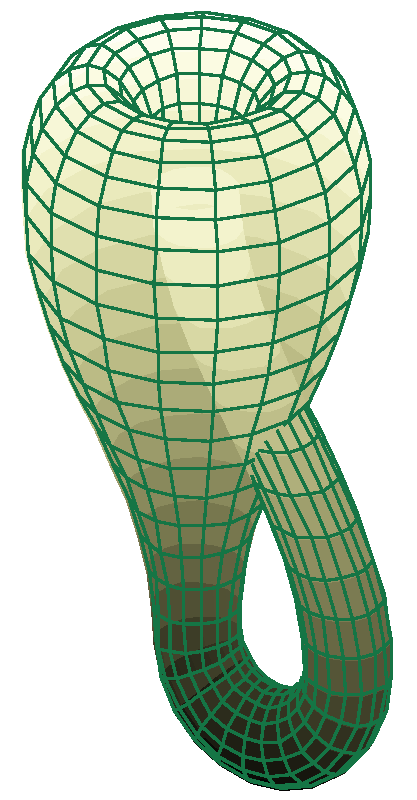
\includegraphics[height=4cm, keepaspectratio]{Bilder/Klein_bottle.pdf}
			\caption[Kleinsche Flasche]{Kleinsche Flasche, \hrefsym{https://en.wikipedia.org/wiki/File:Klein_bottle.svg}{Quelle}}
			}
		\end{figure}
	\end{enumerate}
\end{beispiel}

\begin{satz}[{name=[Zusammenhang der Fundamentalgruppe mit einer e.d.k.-Wirkung]},label=satz:fund-edk]
	Sei $X$ wegzusammenhängend und einfach zusammenhängend. S
	ei $G \action X$ eine e.d.k. Wirkung. 
	Für jedes $\overline{x}_0 \in G \backslash X$ ist dann 
	\[
		\pi_1 \enbrace*{ G \backslash X, \overline{x}_0 } \cong G
	\]
\end{satz}
\begin{beweis}
	Sei $x_0 \in X$ ein Urbild von $\overline{x}_0$, also $\overline{x}_0 = G x_0 $. 
	Zu jeder Schleife $\omega \colon [0,1] \to G \backslash X$ mit $\omega(0) = \omega(1) = \overline{x}_0 $ gibt es eine Hebung $\hat{\omega} \colon [0,1] \to X$ mit $\hat{\omega}(0) = x_0$. 
	Hier heben wir bezüglich der Überlagerung $p \colon X \to G \backslash X$, $x \mapsto G x$, also $p \circ  \hat{\omega} = \omega$.

	Da $p \enbrace*{ \hat{\omega}(1)} = \omega(1) = \overline{x}_0 $ folgt $\hat{\omega}(1)\in p ^{-1} (\overline{x}_0 ) = G  x_0$.  
	Es gibt also $g_\omega \in G$ mit $g_\omega \cdot x_0 = \hat{\omega}(1)$. 
	Wie im Fall der Überlagerung $\mathbb{R} \to S^1$ zeigt man mit Hilfe des Homotopiehebungssatzes, dass $[\omega] \mapsto g_\omega$ ein Gruppenhomomorphismus $\varphi \colon \pi_1(G \backslash X, \overline{x}_0 ) \to G$ definiert. 
	\begin{description}
		\item[Surjektivität von $\varphi$:] Sei $g \in G$. 
		Sei $\hat{\omega} \colon [0,1] \to X$ ein Weg von $x_0$ nach $g \cdot x_0$ (Solch einen Weg gibt es, da $X$ wegzusammenhängend ist). 
		Dann ist $\hat{\omega}$ die Hebung von $\omega \coloneqq p \circ  \hat{\omega}$ und es folgt $\varphi( [\omega]) = g_\omega = g$, da $\hat{\omega}(1) = g \cdot  x_0$. 
		Also $g \in \im \varphi$.
		\item[Injektivität von $\varphi$:] Sei $\omega \coloneqq [0,1] \to G \backslash X$ eine Schleife mit $\omega(0)= \omega(1) = \overline{x}_0$, für die $\varphi([\omega]) = e$. 
		Sei $\hat{\omega} \colon [0,1] \to X$ die Hebung von $\omega$ mit $\hat{\omega}(0) = x_0$. 
		Da $\varphi([\omega]) = e$ ist, gilt $\hat{\omega}(1) = x_0$, $\hat{\omega}$ ist also eine Schleife in $X$. 
		Da $X$ einfach zusammenhängend ist, ist $[\hat{\omega}] = e \in \pi_1(X,x_0)$. 
		Es folgt 
		\[
			[\omega] = [p \circ  \hat{\omega}] = p_* [\hat{\omega}] = p_*(e) = e. \qedhere
		\]
	\end{description}
\end{beweis}

\begin{bemerkung}[{name=[Fundamentalgruppe des reell-projektiven Raumes]}]
	Für $n \ge 1$ ist $S^n$ wegzusammenhängend (einfache Übung).
	Für $n \ge 2$ ist $S^n$ einfach zusammenhängend (weniger einfache Übung).
	
	Nach \cref{satz:fund-edk} ist daher $\pi_1(\mathbb{R}P^n, x_0) = \nicefrac{\mathbb{Z}}{2}$ für $n \ge 2$. 
	Es folgt $\mathbb{R}P^n \not\cong S^n$ für $n \ge 2$. 
	(Andererseits ist $\mathbb{R}P^1 \cong S^1$.)
\end{bemerkung}

\begin{definition}[{name=[Decktransformationen]}]
	Sei $p \colon \hat{X} \to X$ eine Überlagerung. 
	Eine \Index{Decktransformation} von $p$ ist ein Homöomorphismus $f \colon \hat{X} \to \hat{X}$, sodass $p \circ f = p$. 
	Die Decktransformationen von $p$ bilden eine Gruppe $\Delta(p)$. 
	Diese Gruppe wirkt in kanonischer Wiese auf $\hat{X}$.
\end{definition}

\begin{lemma}[{name=[Decktransformationsgruppe wirkt eigentlich diskontinuierlich]}]
	Sei $p \colon \hat{X} \to X$ eine Überdeckung, wobei $\hat{X}$ wegzusammenhängend ist. 
	Dann ist die Wirkung der Decktransformationsgruppe $\Delta(p)$ auf $\hat{X}$ eigentlich diskontinuierlich.
\end{lemma}
\begin{beweis}
	Wir zeigen zunächst, dass die Wirkung frei ist. 
	Sei $f \in \Delta(p)$ und $x \in \hat{X}$ mit $f(x) = x$. Zu zeigen: $f =\id_{\hat{X}}$.
	Sei $y \in \hat{X}$ und $\hat{\omega} \colon [0,1] \to \hat{X}$ ein Weg von $x$ nach $y$. 
	Dann sind $\hat{\omega}$ und $f \circ \hat{\omega}$ zwei Hebungen von $\omega \coloneqq p \circ \hat{\omega}$. 
	Da $\hat{\omega}(0) = x = f(x) = f \circ \hat{\omega}(0)$ folgt mit der Eindeutigkeit im \hyperref[satz:hebung-homotopie]{Homotopiehebungssatz} $\hat{\omega} = f \circ \hat{\omega}$ und insbesondere $y=f(y)$.
	Da $y$ beliebig war, ist $f= \id_{\hat{X}}$.

	Wir können nun zeigen, dass die Wirkung eigentlich diskontinuierlich ist: 
	Sei $x \in \hat{X}$ und $U$ eine elementare Umgebung von $p(x)$. 
	Dann ist $p^{-1}(U)$ die disjunkte Vereinigung von offenen Mengen $V$, $V \in \mathcal{V}$ von denen jede homöomorph auf $U$ abgebildet wird. 
	Sei $V_0 \in \mathcal{V}$ mit $x \in V_0$ und $f \in \Delta(p)$, $f \neq \id$. 
	Für $y \in V_0$ gilt dann $p \enbrace*{f(y)} = p(y)$. 
	Da $f(y) \neq y$ gilt, folgt $f(y) \notin V_0$, denn andernfalls wäre $p\big|_{V_0}$ nicht injektiv. 
	Daher ist $f(V_0) \cap V_0 = \emptyset$.
\end{beweis}

\noindent\begin{minipage}{.82\textwidth}
	\begin{bemerkung}[{name=[Untergruppen der Decktransformationsgruppe]},label=bem:untergrp-decktrans]
		Sei $p \colon \hat{X} \to X$ eine Überlagerung, wobei $\hat{X}$ wegzusammenhängend ist. 
		Sei $H \le \Delta(p)$ eine Untergruppe. Dann ist auch die Wirkung $H \action \hat{X}$ eigentlich diskontinuierlich und die Quotientenabbildung $q \colon \hat{X} \to H \backslash \hat{X}$ eine Überlagerung. 
		Weiter ist $q' \colon H \backslash \hat{X} \to X$ mit $q'(Hx) \coloneqq p(x)$ stetig, da $q' \circ q = p$ stetig ist. 
		Ist $U \subseteq X$ elementar für $p$, so ist $U$ auch elementar für $q'$. 
		$q'$ ist also auch eine Überlagerung.
	
		Insgesamt haben wir also jeder Untergruppe von $\Delta (p)$ eine Überlagerung $H \backslash \hat{X}$ zugeordnet, die zwischen $\hat{X}$ und $X$ liegt.\marginnote{An dieser Stelle darf man sich gerne an die Galois-Gruppen aus \enquote{Einführung in die Algebra} erinnern.}
	\end{bemerkung}
\end{minipage}%
\begin{minipage}{.17\textwidth}
	\hfill\begin{tikzcd}
		\hat{X} \rar{p} \dar{q}& X \\
		H \backslash \hat{X} \urar[swap]{q'}&
	\end{tikzcd}
\end{minipage}

\begin{definition}[{name=[normale Überlagerung]}]
	Sei $p \colon \hat{X} \to X$ eine Überlagerung. 
	Für $x \in X$ wirkt dann $\Delta(p)$ auf $p^{-1}(x)$. 
	Die Überlagerung heißt \bet{normal}\index{Überlagerung!normal}, falls diese Wirkung \emph{transitiv} ist, d.h. falls es zu $\hat{x}, \hat{y} \in p^{-1}(x)$ immer $f \in \Delta(p)$ gibt mit $f(\hat{x})= \hat{y}$.
\end{definition}

\begin{proposition}[{name=[Homöomorphismus für normale Überlagerungen]}]
	Sei $\hat{X} \xrightarrow{p} X $ eine normale Überlagerung, wobei $\hat{X}$ wegzusammenhängend ist. Dann ist die Abbildung
	\mapdef{q' \colon \Delta(p)\backslash \hat{X}}{X}{\Delta(p) x}{p(x)}{\cong}
	Wenn zusätzlich $\hat{X}$ einfach zusammenhängend und wegzusammenhängend ist, dann gilt $\pi_1(X, x_0) \cong \Delta(p)$ für einen beliebigen Basispunkt $x_0 \in X$.
\end{proposition}
\begin{beweis}
	Wir haben in \cref{bem:untergrp-decktrans} schon gesehen, dass $q'$ eine Überlagerung ist unabhängig davon ob $p$ normal ist. Ist $p$ zusätzlich normal, so ist $q'$ eine bijektive Überlagerung und daher automatisch ein Homöomorphismus.
\end{beweis}
% section eigentlich_diskontinuierliche_wirkungen (end)

\newpage
\section{Klassifikation von Überlagerungen} % (fold)
\label{sec:klassifikation_von_uberlagerungen}

\begin{satz}[{name={Hebungssatz}},label=satz:hebungssatz]
	Sei $p \colon \hat{X} \to X$ eine Überlagerung. 
	Sei $x_0 \in X, \hat{x}_0 \in \hat{X}$, $p(\hat{x}_0)= x_0$. 
	Sei $Z$ wegzusammenhängend und lokal wegzusammenhängend. 
	Sei $z_0 \in Z$, $f \colon Z \to X$ stetig mit $f(z_0)= x_0$. 
	Dann gibt es eine Hebung $\hat{f} \colon Z \to \hat{X}$ mit $\hat{f} (z_0) = \hat{x}_0$ genau dann, wenn
	\begin{equation}
		f_*\enbrace[\big]{\pi_1 (Z, z_0)} \subseteq  p_* \enbrace[\big]{\pi_1(\hat{X}, \hat{x}_0)} \tag{$\star$}\label{eq:hebungssatz}
	\end{equation}
	als Untergruppe von $\pi_1(X,x_0)$ gilt. 
	In diesem Fall ist $\hat{f}$ eindeutig.
	\[
		\begin{tikzcd}
			X & \hat{X} \lar[swap]{p} \\
			Z \uar{f}  \urar[dashed, swap]{\hat{f}}&
		\end{tikzcd}
	\]
\end{satz}
\begin{beweis}
	Existiert $\hat{f}$, so folgt \eqref{eq:hebungssatz} aus $f_* = p_* \circ\hat{f}_*$. 
	Sei umgekehrt \eqref{eq:hebungssatz} erfüllt. 
	Sei $z\in Z$. Sei $\omega \colon [0,1]\to Z$ ein Weg von $z_0$ nach $z$.
	Sei $\hat{\omega} \colon [0,1] \to \hat{X}$ die eindeutige Hebung von $f \circ \omega$ mit $\hat{\omega}(0)= \hat{x}_0$ (siehe Homotopiehebungssatz, \ref{satz:hebung-homotopie}). 
	Existiert $\hat{f}$, so ist auch $\hat{f} \circ \omega$ eine Hebung von $f \circ \omega$ mit $\hat{f} \circ \omega (0) = \hat{f}(z_0)= \hat{x}_0$, also $\hat{\omega} = \hat{f} \circ \omega$ und insbesondere ist $\hat{f}(z)= \hat{f} \enbrace[\big]{\omega(1)} = \hat{\omega}(1)$. Daher ist $\hat{f}$ eindeutig, falls es existiert. \smallskip \\
	Zur Existenz setzen wir $\hat{f}(z) := \hat{\omega}(1)$. Wir müssen zeigen:
	\begin{description}
		\item[Wohldefiniertheit:] Sei $\eta \colon [0,1] \to Z$ ein zweiter Weg von $z_0$ nach $z$. 
		Sei $\hat{\eta} \colon [0,1] \to \hat{X}$ die zugehörige Hebung. 
		Zu zeigen: $\hat{\eta}(1) = \hat{\omega}(1)$. 
		Betrachte die Schleife $\overline{\omega} * \eta$ in $Z$. 
		Dann ist $\overline{\hat{\omega}} * \hat{\eta}$ eine Hebung von $f \circ (\overline{\omega} * \eta)$. 
		Aus \eqref{eq:hebungssatz} folgt, dass $\benbrace*{f \circ (\overline{\omega} * \eta )}$ im Bild von $p_* \colon \pi_1(\hat{X}, \hat{x}_0) \to \pi_1(X,x_0)$ liegt. 
		Mit dem Homotopiehebungssatz ergibt sich, dass auch $\overline{\hat{\omega}} * \hat{\eta}$ eine Schleife ist (Übung!). 
		Damit folgt $\hat{\omega}(1)= \hat{\eta}(1)$.
		\item[Stetigkeit:] Sei $U \subseteq \hat{X}$ offen. 
		Sei $z \in \hat{f} ^{-1} (U)$. 
		Sei $V$ eine elementare Umgebung von $f(z)$. 
		Indem wir $V$ wenn nötig klein machen, erhalten wir eine offene Umgebung $V'$ von $\hat{f}(z)$, die unter $p$ homöomorph auf $V$ abgebildet wird. 
		Da $f$ stetig ist und $Z$ lokal wegzusammenhängend ist, gibt es eine wegzusammenhängende Umgebung $W$ von $z$ mit $f(W) \subseteq V$. 
		Sei nun $\omega \colon [0,1] \to Z$ ein Weg von $z_0$ nach $z$.
		Zu $z' \in W$ gibt es einen Weg $\eta \colon [0,1] \to W$ von $z$ nach $z'$ und $\omega * \eta$ ist ein Weg von $z_0$ nach $z'$. 
		Insbesondere ist 
		\[
			\hat{f}(z') = \widehat{(\omega * \eta)} (1)= \hat{\omega} * p\big|_{V'} ^{-1} (\eta) (1) = \enbrace*{p \big|_{V'}} ^{-1} \enbrace[\big]{\eta(1)} \in V'  
		\]
		Also $\hat{f}(W) \subseteq V' \subseteq U$ und $\hat{f}$ ist stetig. \qedhere
	\end{description}
\end{beweis}

\begin{satz}[{name={Eindeutigkeit}}]
	Seien $p_1 \colon \hat{X}_1 \to X$ und $p_2 \colon \hat{X}_2 \to X$ zwei Überlagerungen. 
	Dabei seien $\hat{X}_1$ und $\hat{X}_2$ wegzusammenhängend und lokal wegzusammenhängend.
	Seien $\hat{x}_1 \in \hat{X}_1$, $\hat{x}_2 \in \hat{X}_2$ mit $p_1(\hat{x}_1) = x_0 = p_2(\hat{x}_2)$.
	Dann sind äquivalent:
	\begin{enumerate}[a)]
		\item Es gibt einen Homöomorphismus $f \colon \hat{X}_1 \to \hat{X}_2$ mit $p_2 \circ f = p_1$ und $f(\hat{x}_1) = \hat{x}_2$.
		\item ${p_1}_*\enbrace*{\pi_1 \enbrace*{\hat{X}_1, \hat{x}_1}} = {p_2}_* \enbrace*{\pi_1 \enbrace*{\hat{X}_2, \hat{x}_2}}$ als Untergruppen von $\pi_1(X,x_0)$.
	\end{enumerate}
\end{satz}
\begin{beweis}
	Ist $f$ wie in a), so ist $f_* \colon \pi_1 \enbrace*{\hat{X}_1, \hat{x}_1} \to \pi_1 \enbrace*{\hat{X}_2, \hat{x}_2}$ ein Isomorphismus und es folgt 
	\[
		(p_1)_* \enbrace*{\pi_1 \enbrace*{\hat{X}_1, \hat{x}_1}} =  (p_2 \circ f)_* \enbrace*{\pi_1 \enbrace*{\hat{X}_1, \hat{x}_1}} 
		= (p_2)_* \circ (f)_* \enbrace*{\pi_1 \enbrace*{\hat{X}_1, \hat{x}_1}} = (p_2)_* \enbrace*{\pi_1 \enbrace*{\hat{X}_2, \hat{x}_2}}
	\]
	Für die umgekehrte Implikation betrachte
	\[
		\begin{tikzcd}
			\mbox{ } & \hat{X}_2 \dar{p_2}\\
			\hat{X}_1 \rar{p_1} \urar[dashed]{f}& X
		\end{tikzcd}
	\]
	Nach dem Hebungssatz \ref{satz:hebungssatz} existiert $f \colon \hat{X}_1 \to \hat{X}_2$ mit $p_2 \circ f = p_1$, $f(\hat{x}_1) = \hat{x}_2$. Betrachte nun
	\[
		\begin{tikzcd}
			\mbox{} & \hat{X}_1\dar{p_1} \\
			\hat{X}_2 \rar{p_2} \urar[dashed]{g}&  X
		\end{tikzcd}
	\]
	Wieder liefert der Hebungssatz ein $g \colon \hat{X}_2 \to \hat{X}_1$ mit $p_1 \circ  g = p_2$, $g(\hat{x}_2) = \hat{x}_1$. Betrachte nun
	\[
		\begin{tikzcd}[column sep=4em, row sep=4em]
			\mbox{ } & \hat{X}_1 \dar{p_1}\\
			\hat{X}_1 \rar{p_1} \urar[swap]{\id_{\hat{X}_1}} \urar[bend left]{g \circ f} & X
		\end{tikzcd}
	\]
	Die Eindeutigkeit im Hebungssatz liefert $g \circ f = \id_{\hat{X}_1}$. Analog folgt $f \circ g = \id_{\hat{X}_2}$.
\end{beweis}

\begin{satz}[{name=[universelle Überlagerung]}]
	Sei $X$ wegzusammenhängend, lokal wegzusammenhängend und lokal einfach zusammenhängend. 
	Dann gibt es eine wegzusammenhängende und einfach zusammenhängende  Überlagerung $\tilde{X} \xrightarrow{p} X$.
\end{satz}
\begin{beweis}[Skizze]
	Sei $x_0 \in X$. Sei $P = \set[\big]{{\omega \colon [0,1] \to X \text{ Weg}} \given \omega(0)=x_0} $. Sei 
	\[
		\tilde{X} \coloneqq \sfrac{P}{\text{Homotopie mit festen Endpunkten}}
	\] 
	Dann induziert $\omega \mapsto \omega(1)$ eine wohldefinierte Abbildung $p \colon \tilde{X} \to X$. 
	Sei $\omega \in P$ und $V$ eine wegzusammenhängende, einfach zusammenhängende Umgebung von $\omega(1)$ in $X$. Setze 
	\[
		U(V,\omega) = \set[\big]{{[\omega * \eta]} \given \rule{0cm}{1em} \eta \colon [0,1] \to V \text{ Weg mit } \eta(0)= \omega(1)} 
	\]
	Die $U(V,\omega)$ bilden die Basis der Topologie von $\tilde{X}$. 
	Da $V$ wegzusammenhängend und einfach zusammenhängend ist, ist 
	\[
		p \Big|_{U(V,\omega)} \colon U(V,\omega) \to V
	\]
	bijektiv. 
	Da $X$ lokal wegzusammenhängend und lokal einfach zusammenhängend ist, ist $p \big|_{U(V,\omega)}$ sogar ein Homöomorphismus. 
	Damit ist $V$ eine elementare Umgebung von $\omega(1)$. 
	Da $X$ wegzusammenhängend ist, ist $p$ auch surjektiv und $p \colon \tilde{X} \to X$ eine Überlagerung. 
	
	Zu zeigen bleibt, dass $\tilde{X}$ wegzusammenhängend ist: Sei $\tilde{x}_0 \colon [c_{x_0}] \in \tilde{X}$. 
	Sei $\tilde{x} = [\omega] \in \tilde{X}$. Sei $\omega_s \colon [0,1] \to X$ mit
	\[
		\omega_s(t) = \begin{cases}
			\omega(t), &\text{ falls } t \le s\\
			\omega(s), &\text{ falls } t \ge s
		\end{cases}
	\]
	Dann ist $\alpha \colon [0,1] \to \tilde{X}$ mit $\alpha(s) = [\omega_s]$ ein Weg von $\tilde{x}_0$ nach $\tilde{x}$. 
	Damit ist $\tilde{X}$ wegzusammenhängend.
	Dass $\tilde{X}$ einfach zusammenhängend ist, zeigen wir an dieser Stelle nicht.
\end{beweis}

\begin{definition}[{name=[universelle Überlagerung]}]
	$\tilde{X} \xrightarrow{p} X$ heißt die \bet{universelle Überlagerung}\index{Überlagerung!universell} von $X$.
\end{definition}

\begin{satz}[{name={Existenz}}]
	Sei $X$ wegzusammenhängend, lokal wegzusammenhängend und lokal einfach zusammenhängend. Sei $x_0 \in X$. 
	Dann gibt es zu jeder Untergruppe $H \le \pi_1(X,x_0)$ eine Überlagerung $q \colon \hat{X} \to X$ und $\hat{x}_0 \in p^{-1} (x_0)$ mit $q_* \enbrace*{\pi_1(\hat{X}, \hat{x}_0)} = H$.
\end{satz}
\begin{beweis}
	Sei $p \colon \tilde{X} \to X$ die universelle Überlagerung. 
	Der Hebungssatz\marginnote{Setze dazu $Z=\hat{X}$ in \cref{satz:hebungssatz}} impliziert, dass $p \colon \tilde{X} \to X$ normal ist. 
	Es folgt $\Delta(p) \backslash \tilde{X} \cong X$ und $\pi_1(X, x_0) \simeq \Delta(p)$. 
	Genauer: Zu $\tilde{x}_0 \in p ^{-1}(x_0)$ gibt es einen Isomorphismus $\varphi \colon \Delta (p) \to \pi_1(X,x_0)$ mit 
	\[
		\varphi(f) = [p \circ \tilde{\omega}_f],
	\]
	wobei $\tilde{\omega}_f \colon [0,1] \to \tilde{X}$ ein Weg von $\tilde{x}_0$ nach $f (\tilde{x}_0)$ ist. 
	Setze $H_\Delta \coloneqq \varphi ^{-1}(H)  \le \Delta(p)$. 
	Wir erhalten Überlagerungen $\tilde{X} \xrightarrow{q'} H_\Delta \backslash \tilde{X} \xrightarrow{q} X $ mit $q'(x) = H_\Delta x$ und $q (H_\Delta x) = p(x)$. 
	Da $\tilde{X}$ einfach zusammenhängend ist, ist $\pi_1 \enbrace*{ H_\Delta \backslash \tilde{X}, H_\Delta \hat{x}_0} \cong H_\Delta$ nach \cref{satz:fund-edk}. 
	Sei $\hat{x}_0 \coloneqq H_\Delta \tilde{x}_0$.
	Genauer gibt es einen Isomorphismus
	\mapdef{\psi \colon H_\Delta}{\pi_1 \enbrace*{H_\Delta \backslash \tilde{X}, \hat{x}_0}}{f}{\benbrace*{q' \circ  \omega_f}}{\cong}
	Es folgt 
	\[
		q_* \enbrace[\big]{\psi(f)} = q_* \benbrace*{q' \circ \omega_f} = \benbrace*{q \circ q' \circ \omega_f} = \benbrace*{p \circ \omega_f} = \varphi(f) 
	\]
	Also $q_* \enbrace*{\pi_1 \enbrace*{H_\Delta \backslash \tilde{X}, \hat{x}_0}} = H $. 
	Mit $\hat{X} \coloneqq H_\Delta \backslash \tilde{X}$ folgt die Behauptung.
\end{beweis}
% section klassifikation_von_uberlagerungen (end)

\newpage
\section{Höhere Homotopiegruppen} % (fold)
\label{sec:hohere_homotopiegruppen}
\emph{Dieses Kapitel ist nur ein kleiner Exkurs zu einem Thema, das auch -- mehrere -- Vorlesungen füllen könnte.}\smallskip

Sei $(X,x_0)$ ein punktierter Raum. Sei in diesem Abschnitt $I= [0,1]$.
\begin{description}
	\item[Wegzusammenhang:] Punkte in $X$ können wir auch wie folgt verstehen: $I^0 = \set{x} \to X$. 
	Wege in $X$ sind dann Homotopien solcher Abbildungen. 
	$\pi_0(X,x_0)$ ist dann die (punktierte) Menge der Homotopieklassen von Abbildungen $I^0 \to X$.
	\item[Fundamentalgruppe:] Die Schleifen in $X$ sind stetige Abbildungen $\omega \colon I\to X$ mit $\omega(0)= x_0 = \omega(1)$. 
	$\pi_1(X,x_0)$ ist die Menge der Homotopieklassen von Schleifen und heißt die \Index{Fundamentalgruppe}.
\end{description}
Ziel: Definition von höher dimensionalen Analoga.

\begin{definition}[{name=[Homotopie]}]
	Seien $\omega_0, \omega_1 \colon I^n \to X$ stetige Abbildungen mit $\omega_0(\partial I^n)= \set{x_0} = \omega_1(\partial I^n)$. 
	Eine \Index{Homotopie} (relativ zum Rand) zwischen $\omega_0$ und $\omega_1$ ist eine stetige Abbildung $H \colon I^n \times [0,1] \to X$, sodass Folgendes gilt:
	\begin{itemize}
		\item $H(s_1, \ldots , s_n, 0) = \omega_0(s_1, \ldots , s_n)$ für alle $(s_1, \ldots , s_n) \in I^n$
		\item $H(s_1, \ldots , s_n, 1) = \omega_1(s_1, \ldots , s_n)$ für alle $(s_1, \ldots , s_n) \in I^n$
		\item $H(s_1, \ldots , s_n, t) = x_0$ für alle $t \in [0,1]$, $(s_1, \ldots , s_n) \in \partial I^n$
	\end{itemize}
\end{definition}

Homotopie relativ zum Rand definiert eine Äquivalenzrelation auf der Menge der stetigen Abbildungen $I^n \to X$.
Für $n=1$ erhalten wir die Begriffe aus \cref{sec:die_fundamentalgruppe}.

\begin{definition}[{name=[Höhere Homotopiegruppen]}]
	Sei $(X,x_0)$ ein punktierter Raum. 
	Definiere $\pi_n(X,x_0)$ als die Menge der Homotopieklassen $[\omega]$ von stetigen Abbildungen $\omega \colon I^n \to X$ mit $\omega(\partial I^n)=\set{x_0}$.\marginnote{für $n>0$}
\end{definition}

Wenn wir den Rand auf einen Punkt kollabieren, erhalten wir zum Beispiel für $n=2$:
\[
	\begin{tikzcd}
		I^2 \rar["\omega"] \arrow[d, two heads]& X \\
		\nicefrac{I^2}{\partial I^2} \urar[dashed, "\exists"]
	\end{tikzcd} \qquad \qquad 
	\vcenter{\hbox{\begin{tikzpicture}[scale=0.8]
		\draw (0,0) rectangle (2,2);
		\node at (1,1) {$I^2$};
	\end{tikzpicture}}}
	\enspace\twoheadrightarrow \enspace
	\vcenter{\hbox{
	\begin{tikzpicture}
		\draw (-1,0) arc (180:360:1cm and 0.5cm) node[right]{$S^2$};
	    \draw[dashed] (-1,0) arc (180:0:1cm and 0.5cm);
	    \draw (0,1) arc (90:270:0.5cm and 1cm);
	    \draw[dashed] (0,1) arc (90:-90:0.5cm and 1cm);
	    \draw (0,0) circle (1cm);
	    \shade[ball color=blue!10!white,opacity=0.20] (0,0) circle (1cm);
	\end{tikzpicture}}}
\]
Allgemein erhalten wir für jede stetige Abbildung $\omega \colon I^n \to X$ mit $\omega(\partial I^n) = \set{x_0}$ eine punktierte Abbildung $(S^n, s_0) \to (X,x_0)$.

\begin{definition}[{name=[Analogon zu Kompositionswegen]}]
	Sei $1 \le k \le n$ und seien  $\omega_1, \omega_2 \colon I^n \to X$ stetig mit $\omega_i(\partial I^n) = \set{x_0}$ für $i=1,2$. Definiere:\marginnote{vergleiche \cref{def:kompositionsweg}}
	\[
		\enbrace*{\omega_1 *_k \omega_2} (s_1, \ldots , s_n) \coloneqq \begin{cases}
			\omega_1 \enbrace[\big]{s_1, \ldots , s_{k-1}, 2 s_k, s_{k+1}, \ldots , s_n} &\text{ falls } 0 \le s_k, \le \frac{1}{2} \\
			\omega_2 \enbrace[\big]{s_1, \ldots , s_{k-1}, 2 s_k - 1, s_{k+1}, \ldots , s_n} &\text{ falls } \frac{1}{2} \le s_k \le 1 
		\end{cases} 
	\]
\end{definition}

\begin{lemma}[{name={Eckmann-Hilton-Argument}}]
	Sei $A$ eine Menge mit zwei inneren Verknüpfungen $\boxdot, \diamond \colon A \times A\to A $, sodass gilt:
	\begin{enumerate}[a)]
		\item Es gibt $e \in A$ mit $e \boxdot a = a \boxdot e = a = e \diamond a = a \diamond e$ für alle $a \in A$
		\item Für alle $a,b,c,d \in A$ gilt $(a \boxdot b) \diamond (c \boxdot d) = (a \diamond c) \boxdot (b \diamond d)$.
	\end{enumerate}
	Dann stimmen $\boxdot$ und $\diamond $ überein, sind assoziativ und kommutativ.
\end{lemma}
\begin{beweis}
	Es gilt
	\begin{align*}
		a \boxdot b &= (e \diamond a) \boxdot (b \diamond e) = (e \boxdot b) \diamond (a \boxdot e) = b \diamond a \\
		b \diamond a &= (b \boxdot e) \diamond (e \boxdot a) = (b \diamond e) \boxdot (e \diamond a) = b \boxdot a \\
		a \boxdot (b \boxdot c) &= (a \diamond e) \boxdot (b \diamond c) = (a \boxdot b) \diamond (e \boxdot c) = (a \boxdot b) \boxdot c
	\end{align*}
	Es folgt $\boxdot = \diamond$ und dass die Verknüpfung assoziativ und kommutativ ist.
\end{beweis}

\begin{proposition}[{name=[Gruppenstruktur und induzierte Abbildungen]},label=prop:eig-hom-gruppen]
	Es gilt:
	\begin{enumerate}[a)]
		\item Sei $1 \le k \le n$ und seien $\omega_0, \omega_0', \omega_1, \omega_1' \colon I^n \to X$ stetig mit $\omega_i (\partial I^n) = \set{x_0} = \omega_i'(\partial I^n)$ für $i=0,1$. 
		Es gelte weiter $[\omega_0] = [\omega_1]$ und $[\omega_0'] = [\omega_1']$ in $\pi_n(X,x_0)$. Dann gilt 
		\[
			[\omega_0 *_k \omega_0'] = [\omega_1 *_k \omega_1'] \in \pi_n(X, x_0)
		\]
		Schreibe $\cdot_k$ für die induzierte Verknüpfung.
		\item Seien $1 \le k,l \le n$. Dann gilt $\cdot_k = \cdot_l$. Für $n \ge 2$ ist $\cdot $ kommutativ und außerdem assoziativ.
		\item $\pi_n(X,x_0)$ ist eine abelsche Gruppe für $n \ge 2$.
		\item\label{prop:eig-hom-gruppen:enum:4} Sei $f \colon (X,x_0) \to (Y,y_0)$ stetig. 
		Dann definiert $[\omega] \mapsto [f \circ \omega]$ einen Gruppenhomomorphismus $\pi_n(f) \colon \pi_n(X,x_0) \to \pi_n(Y,y_0)$, falls $n \ge 1$.
		\item Es ist $\pi_n(\id_X) = \id_{\pi_n(X,x_0)}$ und $\pi_n(f \circ g) = \pi_n(f) \circ \pi_n(g)$.
		\item Ist $f$ punktiert homotop zu $g$, so gilt $\pi_n(f) = \pi_n(g)$.
	\end{enumerate}
\end{proposition}
\begin{beweis}
	\begin{enumerate}[a)]
		\item Sei $H$ eine Homotopie zwischen $\omega_0$ und $\omega_1$ und $H'$ eine Homotopie zwischen $\omega_0'$ und $\omega_1'$. 
		Dann ist $H *_k H'$ die gesuchte Homotopie. \hfill (vgl. \cref{lem:eig-kompositionsweg})
		\item Für $n=2$
		\[
			\begin{array}{c}
				(\omega *_1 \omega') \\
				*_2 \\
				(\omega'' *_1 \omega''')
			\end{array}
			 = 
			\vcenter{\hbox{\begin{tikzpicture}[scale=0.9]
				\draw (0,0) grid (2,2);
				\node at (0.5,0.5){$\omega''$};
				\node at (0.5,1.5){$\omega$};
				\node at (1.5,0.5){$\omega'''$};
				\node at (1.5,1.5){$\omega'$};
			\end{tikzpicture}}}
			 = \begin{pmatrix}
			 	\omega \\
				*_2 \\
				\omega''
			 \end{pmatrix} *_1
			 \begin{pmatrix}
			 	\omega' \\
				*_2 \\
				\omega'''
			 \end{pmatrix}
		\]
		Mit dem Eckmann-Hilton-Argument folgt $\cdot_k = \cdot_l$, die Kommutativität und die Assoziativität.
		\item Nur die Existenz von Inversen muss noch gezeigt werden:
		Gegeben $\omega \colon I^n \to X$. Wähle $1 \le k \le n$ und setze
		\[
			\overline{\omega} (s_1, \ldots , s_n) \coloneqq \omega  \enbrace[\big]{s_1, \ldots , s_{k-1} ,1- s_k , s_{k+1}, \ldots , s_n} 
		\]
		Dann ist $[\overline{\omega}]$ das Inverse von $[\omega]$, da $[\overline{\omega} *_k \omega ]$ nullhomotop ist.
		\item[d)--f)] einfach. \qedhere
	\end{enumerate}
\end{beweis}

\begin{korollar}[{name=[Die Homotopiegruppen punktiert homöomorpher Räume stimmen überein]}]
	Es gilt 
	\[
		(X,x_0) \simeq (Y,y_0) \implies \pi_n(X,x_0) \cong \pi_n(Y,y_0)
	\]
	für alle $n$. Insbesondere ist $\pi_n(X,x_0) = 0$ für $n \ge 2$, wenn  $(X,x_0)$ zusammenziehbar ist.
\end{korollar}

\begin{proposition}[{name=[für $n\ge 2$ induzieren Überlagerungen Gruppenisomorphismen]},label=prop:iso-covering]
	Sei $p \colon \hat{X} \to X$ eine Überlagerung und $\hat{x}_0 \in \hat{X}, x_0 \in X$ mit $p(\hat{x}_0) = x_0$ Basispunkte. Dann ist $\pi_n(p) \colon \pi_n(\hat{X}, \hat{x}_0) \to \pi_n(X,x_0)$ ein Isomorphismus für $n \ge 2$.
\end{proposition}
\begin{beweis}
	\emph{Übung: Blatt 10 Aufgabe 3, siehe Anhang \hyperref[sub:B10A3]{\ref*{sub:B10A3} auf Seite \pageref*{sub:B10A3}}.}
\end{beweis}

\begin{korollar}[{name=[höhere Homotopiegruppen der 1-Sphäre]}]
	Es ist $\pi_n(S^1, s_0) = 0$ für $n \ge 2$.
\end{korollar}
\begin{beweis}
	Es gibt eine Überlagerung $\mathbb{R} \to S^1$. 
	Da $\mathbb{R}$ zusammenziehbar ist, folgt die Behauptung aus \cref{prop:iso-covering}.
\end{beweis}

\begin{definition}[{name=[Faserung]}]
	Eine stetige Abbildung $p \colon E \to B$ heißt (Serre-)\Index{Faserung}, falls sie folgende Homotopiehebungseigenschaft hat: 
	Für jedes $n \ge 0$, jede Homotopie $H \colon I^n \times [0,1] \to B$ und jede partielle Hebung $\tilde{H} \colon I^n \times \set{0} \cup \partial I^n \times [0,1]$ existiert eine Hebung $\overline{H}$ von $H$ entlang $p$, die $\tilde{H}$ fortsetzt. Nenne $p^{-1}(b)$ die \Index{Faser} über $b$. 
	\[
		\begin{tikzcd}[row sep=3em, column sep=3em]
			I^n \times \set{0} \cup \partial I^n \times [0,1] \rar["\tilde{H}"]  \dar[hook]& E \dar["p"] \\
			I^n \times [0,1] \rar["H"] \urar[dashed,"\overline{H}"]& B
		\end{tikzcd}
	\]
\end{definition}

Man überlegt sich, dass Überlagerungen Faserungen sind(!).
Ein weiteres triviales Beispiel für eine Faserung ist die Projektion $B \times F \to B$.

\begin{satz}[{name=[lange Homotopiesequenz]}]
	Sei $p \colon E \to B$ eine Faserung. 
	Seien $b_0 \in B, e_0 \in E$ mit $p(e_0)= b_0$. 
	Setze $F \coloneqq p ^{-1}(b_0)$. 
	Sei $i \colon (F, e_0) \hookrightarrow (E,e_0)$ die Inklusion.
	Dann existiert eine lange exakte Sequenz
	\[
		\begin{tikzcd}[row sep=1em]
			\ldots  \pi_{n+1}(B,b_0) \rar["\partial_{n+1}"] & \pi_n(F,e_0) \rar["\pi_n(i)"] & \pi_n(E,e_0) \rar["\pi_n(p)"]& \pi_n(B,b_0)  \rar["\partial_n"]& \pi_{n-1}(F,e_0) \ldots  \\
			\qquad \ldots  \qquad  \rar & \pi_1(B,b_0) \rar["\partial_1"] & \pi_0(F,e_0) \rar["\pi_0(i)"]& \pi_0(F,e_0) \rar["\pi_0(p)"]& \pi_0(B,b_0)
		\end{tikzcd}
	\]
	Das heißt
	\begin{itemize}
		\item $\partial_n$ ist ein Homomorphismus für $n >2$
		\item $\ker \pi_n(p) = \im \pi_n(i)$, $\ker( \partial_{n+1}) = \im \pi_{n+1}(p)$, $\ker \pi_n(i) = \im \partial_{n+1}$ für $n \ge 1$
		\item $\partial_1(x) = [e_0] \iff x \in \im \pi_1(p)$
		\item $\pi_0(i)(x) = [e_0] \iff x \in \im \partial_1$
		\item $\pi_0(p)(x) = [b_0] \iff x \in \im \pi_0 (i)$
	\end{itemize}
\end{satz}
\begin{beweis}
	Definition von $\partial_n$: Sei $\omega \colon I^n \to B$ mit $\omega(\partial I^n) = \set{b_0}$. 
	Fasse $\omega$ als Homotopie $I^{n-1} \times [0,1] \to B$ auf.
	Dann ist die konstante Abbildung $\mathrm{const}_{e_0} \colon I^{n-1} \times \set{0} \cup \partial I^{n-1} \times [0,1] \to E$ mit Wert $e_0$ eine partielle Hebung.
	Da $p$ eine Faserung ist, existiert eine Hebung $\tilde{\omega} \colon I^{n-1} \times [0,1] \to E$, die $\mathrm{const}_{e_0}$ fortsetzt.
	\[
		\begin{tikzcd}[row sep=3em, column sep=4em]
			I^{n-1} \times \set{0} \cup \partial I^{n-1} \times [0,1] \rar["\mathrm{const}_{e_0}"] \dar[hook]& E \dar["p"] \\
			I^{n-1} \times [0,1] \rar["\omega"] \urar[dashed,"\tilde{\omega}"]& B 
		\end{tikzcd}
	\]
	Definiere nun $\partial_n([\omega]) \coloneqq \benbrace*{\tilde{\omega}|_{I^{n-1} \times \set{1}}}$.
	\begin{description}
		\item[Wohldefiniertheit:] Seien $\omega, \omega' \colon I^n \to B$ mit $[\omega]=[\omega']$, d.h. es gibt eine Homotopie $H \colon I^n \times [0,1] \to B$ zwischen $\omega$ und $\omega'$. Sei 
		\[
			J \coloneqq I^{n-1} \times \set{0} \times [0,1] \quad \cup \quad I^n \times\set{0}\quad\cup\quad I^n \times\set{1}\quad \cup \quad \partial I^{n-1} \times I \times [0,1]  
		\]
		Diese Menge ist homöomorph zu $I^n \times \set{0} \cup \partial I^n \times [0,1]$ unter dem Homöomorphismus $I^{n+1} \cong I^{n+1}$, der die letzte und vorletzte Koordinate vertauscht.
		\begin{figure}[htbp]
			\centering{\qquad \qquad 
			\begin{tikzpicture}[draw/.append style=thick, scale=0.9]
				% draw the left part
				\draw (0,0,-4) rectangle (1,1,-4);
				\draw[dashed] (0,0) -- (0,0,-4);
				\draw (1,1) -- (1,1,-4);
				\draw (0,1) -- (0,1,-4);
				\draw (1,0) -- (1,0,-4);
				\draw[decorate, 
					decoration={brace,amplitude=5pt, mirror, raise=3pt}, 
					] (1,0) -- (1,0,-4) node[below right, midway, xshift=0.2cm]{$[0,1]$};
				\draw[decorate, 
					decoration={brace,amplitude=5pt, mirror, raise=3pt}, 
					] (0,0) -- (1,0) node[below, midway, yshift=-0.2cm]{$I^2$};
				\draw (0,0) rectangle (1,1);
		
				% draw right part
				\draw[SpringGreen4, fill=SpringGreen3!40, fill opacity=0.3] (8,0,-4.5) rectangle (9,1,-4.5);
				\node[SpringGreen4,right] at (9,0.5,-4.5) {$I^2 \times \set{1}$};
		
		
				\draw[Firebrick2, fill=Firebrick1!40, fill opacity=0.3] (7.3,0) -- (7.3,1) -- (7.3,1,-4) -- (7.3,0,-4) -- cycle ;
				\node[above left, Firebrick2] at (7.3,1,-2) {$I \times \set{0} \times [0,1]$};
		
				\draw[RoyalBlue3, fill=RoyalBlue2!40, fill opacity=0.3] (8,-0.5) -- (9,-0.5) -- (9,-0.5,-4) -- (8,-0.5,-4) -- cycle ;
				\node[RoyalBlue3, below right] at (9,-0.5,-2) {$\partial I \times I \times [0,1]$} ;
		
				\draw[SpringGreen4, fill=SpringGreen3!40, fill opacity=0.3] (8,0,0.5) rectangle (9,1,0.5);
				\node[SpringGreen4,below left] at (8,0,0.5) {$I^2 \times \set{0}$};
		
				\draw[RoyalBlue3, fill=RoyalBlue2!40, fill opacity=0.3] (8,1.5) -- (9,1.5) -- (9,1.5,-4) -- (8,1.5,-4) -- cycle ;
			\end{tikzpicture}
			\caption{Die Menge $J$ für $n=2$}}
		\end{figure}
		Wir können eine partielle Hebung $\bar{H} \colon J \to E$ von $H$ definieren, indem wir $\bar{H} \big|_{I^n \times \set{0}} = \tilde{\omega}$ und $\bar{H} \big|_{I^n \times \set{1}} = \tilde{\omega'}$ setzen und $\bar{H}$ sonst konstant $e_0$ sein lassen ($\tilde{\omega}$ und $\tilde{\omega'}$ sind gewählte Hebungen von $\omega$ und $\omega'$). 
		Nach der Vorbemerkung über $J$ können wir $\bar{H}$ zu einer Hebung $\tilde{H}$ von $H$ fortsetzen. 
		Dann ist $\tilde{H} |_{I^{n-1} \times \set{1} \times [0,1] }$ eine Homotopie zwischen $\tilde{\omega} |_{I^{n-1} \times \set{1}}$ und $\tilde{\omega'} |_{I^{n-1} \times \set{1}}$ in $F$.
		\item[Homomorphismus:] Wir betrachten Exaktheit nur an den Stellen, an denen alle beteiligten Abbildungen Homomorphismen sind.
		\item[Exaktheit bei $\pi_n(E,e_0)$:] Sei $[\omega ] \in \pi_n(F, e_0)$. 
		Dann ist $p \circ i \circ \omega \equiv b_0$, also $\im \pi_n (i) \subseteq \ker \pi_n(p)$.
	
		Sei nun $[\omega ] \in \pi_n(E, e_0)$, sodass eine Homotopie $H \colon I^n \times [0,1] \to B$ zwischen $p \circ \omega$ und $\mathrm{const}_{b_0}$ existiert, also $[\omega] \in \ker \pi_n(p)$. 
		Indem wir $\omega$ durch die konstante Abbildung auf $I^n \times \set{0} \cup \partial I^n \times [0,1]$ fortsetzen, können wir die Homotopiehebungseigenschaft anwenden und erhalten eine Hebung $\bar{H}$ von $H$. 
		Diese Hebung ist eine Homotopie zwischen $\omega$ und $\omega' \coloneqq \bar{H} |_{I^n \times \set{1} }$. 
		Da $p \circ \omega' = \mathrm{const}_{b_0}$, ist $\omega' \colon I^n \to F$. 
		Also $\im \pi_n(i) \subseteq \ker \pi_n(p)$.
		\item[Exaktheit bei $\pi_n(B, b_0)$:] Sei $\omega \colon I^n \to E$. 
		Dann ist $\omega$ selbst eine zulässige Hebung für $p \circ \omega$, wie wir sie in der Definition von $\partial_n$ benutzt haben. 
		Also ist
		\[
			\partial_n \enbrace*{[p \circ \omega]} = \benbrace*{\omega |_{I^{n-1} \times \set{1}}}  = \benbrace*{\mathrm{const}_{e_0}}, 
		\]
		d.h. $\im \pi_n(p) \subseteq \ker \partial_n$.
	
		Gelte nun $[\omega] \in \ker \partial_n$, d.h.\marginnote{Notation wie in Def. von $\partial_n$} es gibt eine Homotopie $H$ zwischen $\tilde{\omega}|_{I^{n-1} \times\set{1}}$ und $\mathrm{const}_{e_0}$ in $F$.
		Dann definiert $[\tilde{\omega} *_n H]$ ein Element in $\pi_n(E,e_0)$ und $p \circ (\tilde{\omega} *_n H) = \omega *_n \mathrm{const}_{b_0}$, da $H$ eine Homotopie in n$F$ ist. 
		Also gilt $\ker \partial_n \subseteq \im \pi_n(p)$.
		\item[Exaktheit bei $\pi_n(F, e_0)$:] Sei $[\omega] \in \pi_n(B,b_0)$. 
		Wähle $\tilde{\omega}$ wie in der Definition von $\partial_n$. 
		Dann ist $\tilde{\omega}$ eine Homotopie zwischen $i \circ \tilde{\omega} |_{I^{n-1} \times \set{1}}$ und $\mathrm{const}_{e_0}$, also $\im \partial_{n+1} \subseteq \ker \pi_n(i)$.
	
		Sei nun $[\omega] \in \pi_n(F,e_0)$, sodass eine Homotopie $H \colon I^n \times [0,1] \to E$ zwischen $i \circ \omega$ und $\mathrm{const}_{e_0}$ existiert. 
		Diese Homotopie ist eine Hebung von $p \circ H$, die zeigt, dass $\partial_{n+1} \enbrace*{ [p \circ H]} = [\omega]$. 
		Also $\ker \pi_n(i) \subseteq \im \partial_{n+1}$. \qedhere
	\end{description}
\end{beweis}

Diesen Satz kann man wie folgt anwenden:
Es gibt eine Faserung $S^3 \xrightarrow{p} S^2$, sodass $p^{-1}(s) \cong S^1$ (\enquote{Hopf-Faserung}\index{Hopf-Faserung}). 
Es gilt $\pi_1(S^n)= 1$ für $n \ge 2$ und $\pi_2(S^3)= 0$.
Betrachte nun:
\begin{align*}
	\ldots  &\longrightarrow \underbrace{\pi_3(S^1)}_{=0} \longrightarrow \pi_3(S^3) \longrightarrow \pi_3(S^2) \longrightarrow \underbrace{\pi_2(S^1)}_{=0} \\
	&\longrightarrow \underbrace{\pi_2(S^3)}_{=0} \longrightarrow \pi_2(S^2) \longrightarrow \pi_1(S^1) \longrightarrow \underbrace{\pi_1(S^3)}_{=1} \longrightarrow \ldots 
\end{align*}
Mit Exaktheit folgt $\pi_2(S^2) \cong \pi_1(S^1) \cong \mathbb{Z}$ und $\pi_3(S^3) \cong \pi_3(S^2)$. 
Tatsächlich gilt sogar $\pi_3(S^3) \cong \mathbb{Z}$.
% section hohere_homotopiegruppen (end)

\newpage
\section{Differenzierbare Mannigfaltigkeiten} % (fold)
\label{sec:differenzierbare_mannigfaltigkeiten}

Sei $M$ eine topologische Mannigfaltigkeit. 
Welche Funktionen $f \colon M \to \mathbb{R}$ sind differenzierbar? 
Was sind Richtungsableitungen für solche Funktionen? 
Was sind Richtungen in $M$?

Da topologische Mannigfaltigkeiten lokal homöomorph zum $\mathbb{R}^n $ wäre folgendes ein naheliegender Ansatz für eine Definition im obigen Sinne:
$f \colon M \to \mathbb{R}$ heißt $C^\infty$ genau dann, wenn
\[
	\forall x \in M : \exists  U \subseteq M \text{ offen mit } x \in U \text { und } h \colon U \xrightarrow{\approx}  V \subseteq \mathbb{R}^n : f \circ h ^{-1} : V \to \mathbb{R} \text{ ist } C^\infty
\]
Dieser Ansatz hat aber noch die folgenden Probleme:
\begin{enumerate}[a)]
	\item Ob $f \circ h ^{-1} \colon V \to \mathbb{R}$ $\, C^\infty$ ist oder nicht, hängt von der Wahl von $h$ ab.
	\item Jeder Homöomorphismus $f \colon \mathbb{R} \to \mathbb{R}$ ist in dieser Definition $C^\infty$!
\end{enumerate}

\begin{definition}[{name=[{Karten, Kartenwechsel, Atlanten}]}]
	Sei $M^n$ eine topologische $n$-Mannigfaltigkeit. 
	\begin{enumerate}[a)]
		\item Eine \Index{Karte} für $M$ ist ein Homöomorphismus $h \colon U \xrightarrow{\approx}V$ mit $U \subseteq M$ offen, $V\subseteq\mathbb{R}^n$ offen. 
		$U$ heißt das \Index{Kartengebiet} von $h$. 
		Ist $x \in U$, so heißt $h$ eine \bet{Karte um} $x$.
		\item Sind $h_i \colon U_i \xrightarrow{\approx} V_i$, $i=0,1$ zwei Karten, so heißt 
		\[
			h_1 \circ h_0 ^{-1}\big|_{h_0(U_0 \cap U_1)} \colon \underset{\subseteq V_0 \subseteq \mathbb{R}^n}{h_0(U_0 \cap U_1)} \to \underset{\subseteq V_1 \subseteq 
			\mathbb{R}^n}{h_1 (U_0 \cap U_1)}
		\]
		der \Index{Kartenwechsel} zwischen $h_0$ und $h_1$. 
		Ein Kartenwechsel ist ein Homöomorphismus zwischen offenen Teilmengen des $\mathbb{R}^n$. 
		\item Eine Menge von Karten $\set[\big]{h_\alpha : U_\alpha \to V_\alpha \given \alpha \in A}$ heißt ein \Index{Atlas} für $M$, wenn die Kartengebiete $U_\alpha$ die Mannigfaltigkeit überdecken:
		\(
			M = \bigcup_{\alpha \in A} U_\alpha
		\)
		\item Ein Atlas $\mathcal{A}$ heißt $C^\infty$ (oder \bet{glatt}\index{Atlas!glatter}), wenn alle Kartenwechsel zwischen Karten aus $\mathcal{A}$ $C^\infty$"=Abbildungen sind.
	\end{enumerate}
\end{definition}

\begin{definition}[{name=[differenzierbare Mannigfaltigkeit]}]
	Eine \bet{$C^\infty$"=Mannigfaltigkeit}\index{C-Mannigfaltigkeit@$C^\infty$-Mannigfaltigkeit} ist eine topologische Mannigfaltigkeit zusammen mit einem $C^\infty$"=Atlas $\mathcal{A}$.
\end{definition}

\begin{beispiel}[{name=[differenzierbare Mannigfaltigkeiten]}]
	Viele interessante topologische Räume sind differenzierbare Mannigfaltigkeiten:
	\begin{enumerate}[(1)]
		\item $U \subseteq \mathbb{R}^n$ offen ist eine $C^\infty$"=Mannigfaltigkeit mit Atlas $\set{\id_U}$.
		\item $S^n$ ist eine $C^\infty$"=Mannigfaltigkeit: 
		Definiere Kartengebiete $U_{k,j} \coloneqq \set[\big]{x \in S^n \given (-1)^j x_k > 0}$ für $k=0, \ldots, n$, $j=0,1$. Sei 
		\[
			h_{k,j} \colon U_{k,j} \to \interior{D}^n = \set[\big]{x \in \mathbb{R}^n \given \norm{x}_2 < 1 } 
		\]
		mit 
		\[
			h_{k,j} (x_0, \ldots , x_n) = (x_0, \ldots , x_{k-1}, x_{k+1}, \ldots , x_n)
		\]
		Dann ist $\mathcal{A} = \set[\big]{h_{k,j} \given k=0, \ldots ,n \enspace j=0,1}$ ein $C^\infty$"=Atlas für $S^n$.
		\begin{figure}[htbp]
			\centering{
			\tikzsetnextfilename{sphere_S2}
			\begin{tikzpicture}[scale=1.5]
				\begin{scope}
					\clip (-1,0) arc (180:360:1cm and 0.5cm) arc (0:180:1cm and 0.5cm);
		  		  	\foreach \x in {-1.1,-1, -0.9,-0.8,...,1,1.1}%
		  		    	\draw[Sienna3!80,line width=0.3mm](\x,0,2)--(\x,0,-2);
				\end{scope}
				\draw (-1,0) arc (180:360:1cm and 0.5cm);
			    \draw[dashed] (-1,0) arc (180:0:1cm and 0.5cm);
			    \draw (0,1) arc (90:270:0.5cm and 1cm);
			    \draw[dashed] (0,1) arc (90:-90:0.5cm and 1cm);
			    \draw (0,0) circle (1cm);
			    \shade[ball color=blue!10!white,opacity=0.20] (0,0) circle (1cm);
				\draw[dashed, ->] (-1.2,0) -- (1.3,0) node[right]{$x_2$};
				\draw[dashed, ->] (0,-1.2) -- (0,1.3) node[right]{$x_3$};
				\draw[dashed, ->] (0,0,-2) -- (0,0,2.5) node[below]{$x_1$};
				\node[left] at (-.8,.8) {$S^2$};
				\draw[decorate, decoration={brace,amplitude=5pt, mirror, raise=4pt},yshift=0pt, thick] (1.8,0) -- (1.8,1) node[right, midway, xshift=0.25cm]{$U_{3,0}$};
				\node[color=Sienna3] at (0,-1.4) {$h_{3,0}(U_{3,0}) = \set[(x_0,x_1)]{x_0^2+ x_1^2 < 1} $};
			\end{tikzpicture}
			\caption{Die $C^\infty$"=Mannigfaltigkeit $S^2$ mit dem Kartengebiet $U_{3,0}$}}
		\end{figure}
		\item \label{154:enum:3} $\mathbb{R}P^n = \nicefrac{S^n}{x \sim -x}$ ist eine $C^\infty$"=Mannigfaltigkeit: Setze 
		\[
			U_k \coloneqq \set[\big]{{\benbrace[\big]{(x_0, \ldots, x_n)} \in \mathbb{R}P^n} \given x_k \neq 0} 
		\]
		und definiere $h_k \colon U_k \to \interior{D}^n$ durch
		\[
			h_k \enbrace[\big]{[x_0, \ldots, x_n]} = \frac{x_k}{\abs*{x_k}} \enbrace*{x_0, \ldots , x_{k-1}, x_{k+1}, \ldots, x_n} 
		\]
		Dann ist $\set{h_k \given k=0, \ldots, n}$ ein $C^\infty$"=Atlas für $\mathbb{R}P^n$.
		\item Sind $(M, \mathcal{A})$ und $(N, \mathcal{B})$ $C^\infty$"=Mannigfaltigkeiten, so ist $\set{h \times k \given h \in \mathcal{A}, k \in \mathcal{B}}$ ein $C^\infty$"=Atlas für $M \times N$.
	\end{enumerate}
\end{beispiel}

\begin{bemerkung}[{name=[maximaler Atlas]}]
	Sei $(M,\mathcal{A})$ eine $C^\infty$"=Mannigfaltigkeit. 
	Eine Karte $h \colon U \to V$ für $M$ (nicht notwendig in $\mathcal{A}$) heißt eine $C^\infty$"=Karte, wenn alle 
	Kartenwechsel zwischen $h$ und einer Karte aus $\mathcal{A}$ $C^\infty$ sind. 
	Offenbar besteht $\mathcal{A}$ aus $C^\infty$"=Karten. 
	Es ist auch $\mathcal{A}_\mathrm{max}\coloneqq \set[\big]{h \given h \text{ ist $C^\infty$"=Karte}}$ ein $C^\infty$"=Atlas für $M$. 
	Dieser Atlas ist maximal, d.h. man kann keine weiteren Karten zu $\mathcal{A}_\mathrm{max}$ hinzufügen und immer noch einen $C^\infty$"=Atlas erhalten.\index{Atlas!maximaler}
\end{bemerkung}

\begin{definition}[{name=[Differenzierbarkeit von Abbildungen zwischen Mannigfaltigkeiten]}]
	Seien $M,N$ $C^\infty$"=Mannigfaltigkeiten. 
	Sei $f \colon M \to N$ eine stetige Abbildung.
	\begin{enumerate}[a)]
		\item Sei $x \in M$. 
		$f$ heißt $C^\infty$ oder \bet{glatt}\index{Differenzierbarkeit} in $x$, wenn es eine Karte $h_0 \colon U_0 \to V_0$ von $M$ um $x$ und eine Karte $h_1 \colon U_1 \to V_1$ von $N$ um $f(x)$ gibt, sodass 
		\[
			h_1 \circ f \circ h_0 ^{-1}
		\]
		auf einer Umgebung von $h_0(x)$ eine $C^\infty$"=Abbildung ist.
		\item Ist $f$ in allen $x \in M$ glatt, so heißt $f$ eine \bet{$C^\infty$"=Abbildung}\index{C-Abbildung@$C^\infty$"=Abbildung}. 
		Wir schreiben $C^\infty(M,N)$ für die Menge der $C^\infty$"=Abbildungen von $M$ nach $N$.
		\item $M$ und $N$ heißen \Index{diffeomorph} ($\cong$), wenn es $f \in C^\infty(M,N)$ und $g \in C^\infty(N,M)$\marginnote{$\approx$ homöomorph\linebreak$\cong$ diffeomorph} gibt mit $f \circ g = \id_N$ und $g \circ f = \id_M$. 
	
		In diesem Fall heißen $f$ und $g$ \Index{Diffeomorphismen}. 
	\end{enumerate}	
\end{definition}

Man etwas künstliches Beispiel:
$(M,\mathcal{A})$ und $(M, \mathcal{A}_\mathrm{max})$ sind diffeomorph mittels der Identität $\id_M \colon (M,\mathcal{A}) \to (M, \mathcal{A}_\mathrm{max})$.

\begin{bemerkung}[{name=[zur Definition von Differenzierbarkeit]}]
	Einige Anmerkungen zur obigen Definiton von Differenzierbarkeit:
	\begin{enumerate}[a)]
		\item Ist $f \colon M \to N$ glatt in $x$, so ist $h_1 \circ f \circ h_0 ^{-1}$ glatt in einer Umgebung von $h_0(x)$ für \emph{alle} Wahlen von $C^\infty$"=Karten $h_0$ um $x$ und $h_1$ um $f(x)$.
		\item Die Komposition von $C^\infty$"=Abbildungen ist wieder eine $C^\infty$"=Abbildung.
		\item Ist $f \colon M \to N$ bijektiv und $C^\infty$ ist, so ist $f$ noch nicht notwendigerweise ein Diffeomorphismus. (betrachte z.B. $f \colon \mathbb{R} \to \mathbb{R}$, $x \mapsto x^3$)
	\end{enumerate}
\end{bemerkung}

\begin{bemerkung}[{name=[Homöomorphismen und Diffeomorphismen]}]
	Beim Unterscheiden zwischen Homöomorphismen und Diffeomorphismen ist Vorsicht geboten:
	\begin{enumerate}[a)]
		\item Es gibt $C^\infty$"=Mannigfaltigkeiten $M$ und $N$, sodass $M$ und $N$ zueinander homöomorph sind, aber nicht diffeomorph sind. Dabei kann man sogar $M=S^7$ wählen.
		\item Es gibt topologische Mannigfaltigkeiten, auf denen kein $C^\infty$"=Atlas existiert.
	\end{enumerate}
\end{bemerkung}

\begin{definition}[{name=[Untermannigfaltigkeit]},label=def:untermfkt]
	Eine Teilmenge $N \subseteq M^{n+k}$ einer $(n+k)$-dimensionalen $C^\infty$"=Mannigfaltigkeit $M$, heißt eine $n$ dimensionale $C^\infty$"=\Index{Untermannigfaltigkeit}, wenn es um jedes $x \in N$ eine Karte $h \colon U \to V \subseteq \mathbb{R}^{n+k}$ für $M$ gibt, so dass $h(N \cap U) = V \cap (\mathbb{R}^n \times \set{0})$.
	$k= \dim M - \dim N$ heißt die \Index{Kodimension} von $N$ in $M$. 
	Durch Einschränkung dieser Karten von $M$ auf $N$ erhalten wir einen $C^\infty$"=Atlas für $N$. 
	Insbesondere ist $N$ eine $n$-dimensionale $C^\infty$"=Mannigfaltigkeit.
\end{definition}

\begin{figure}[tbhp]
	\centering{ \tikzsetnextfilename{Untermannigfaltigkeit}
	\begin{tikzpicture}[scale=1.2]
		% \draw[help lines] (0,0) grid (8,4);
		\coordinate (x) at (2,2);
		\path (5,1) coordinate (ecke)  +(1,0) node[below]{$V \subseteq \mathbb{R}^2$} ++(0,1) coordinate(start) ++(1,0) coordinate(mitte); % 
		\coordinate (e1) at (1.4,1.35);
		\draw[very thick, DodgerBlue3] (0,0) .. controls +(120:0.6) and +(200:0.5) .. (0,1.5)
			.. controls +(20:0.4) and +(170:0.7) .. (x) 
			.. controls +(-10:1) and +(90:0.5) .. (3,1)
			.. controls +(-80:0.6) and +(-10:0.3) .. (2.2,0.4) node[below]{$N$}
			.. controls +(170:0.5) and +(120:0.4) .. (1.5,-0.5)
			.. controls +(-60:1) and +(-60:0.7) .. cycle ;
		\draw[fill=Tomato2] (x) circle(0.05) node[below]{$x$};
		\draw[very thick, DodgerBlue3] (start) -- ++(2,0) node[right]{$\mathbb{R} \times \set{0}$};
		\draw[fill=Tomato2] (mitte) circle(0.05) node[below]{$h(x)$};
		\draw[very thick, Sienna3] (ecke) rectangle ++(2,2);
		\draw[very thick, Sienna3] (e1) .. controls +(90:0.4) and +(-70:0.4) ..
			++(100:1.2) .. controls +(20:0.5) and +(150:0.4) .. 
			++(-4:1.5) .. controls +(250:0.4) and +(95:0.4) .. 
			++(-0.1,-1.2) .. controls +(160:0.4) and +(10:0.4) .. cycle;
		\draw[-to, thick] (3,2) -- ++(1.8,0) node[midway, above]{$h$};
	\end{tikzpicture}
	\caption{Skizze einer Untermannigfaltigkeit $N$ der Mannigfaltigkeit $M=\mathbb{R}^2$}}
\end{figure}

\begin{definition}[{name=[Einbettung]}]
	Eine $C^\infty$"=Abbildung $f \colon N \to M$ heißt eine \Index{Einbettung}, wenn $f(N) \subseteq M$ eine $C^\infty$"=Untermannigfaltigkeit ist und $f \colon N \to f(N)$ ein Diffeomorphismus ist. 
\end{definition}
% section differenzierbare_mannigfaltigkeiten (end)

\newpage
\section{Reguläre Werte} % (fold)
\label{sec:regulare_werte}

Man betrachte, die in \cref{fig:height-torus} gezeichnete Höhenfunktion auf dem Torus $T^2$.
Wie angedeutet, scheinen die Urbilder einzelner Punkte Mannigfaltigkeiten zu sein, die entweder $S^1$ oder eine disjunkte Vereinigung von zwei Kopien der $S^1$ sind.
An zwei Punkten (einer davon der grün gezeichnete) findet ein Wechsel zwischen diesen beiden Typen von Urbildern statt und das Urbild ist \texttt{keine} Mannigfaltigkeit, da eine Umgebung des Klebepunktes der beiden 1-Sphären nicht homöomorph zum $\mathbb{R}^1$ ist.
\begin{figure}[htbp]
	\centering{
	\begin{tikzpicture}[rotate=90, xscale=0.8, yscale=1, scale=0.7]
		% \draw[help lines] (-4,-4) grid (4,4);
		\draw[->] (-4,-7) -- (4,-7) node[above]{$\mathbb{R}$};
		
		\draw[RoyalBlue2, thick] (-2.5,1.89) .. controls +(240:0.8) and +(120:0.8) .. (-2.5,-1.89);
		\draw[RoyalBlue2, thick, dashed] (-2.5,1.89) .. controls +(300:0.8) and +(60:0.8) .. (-2.5,-1.89);
		\draw[fill=RoyalBlue2] (-2.5,-7) circle[radius=0.07];
		
		\draw[Firebrick2, thick] (0,2.5) .. controls +(250:0.6) and +(110:0.6) .. (0,0.5);
		\draw[Firebrick2, thick, dashed] (0,2.5) .. controls +(290:0.6) and +(70:0.6) .. (0,0.5);
		
		\draw[Firebrick2, thick] (0,-0.5) .. controls +(250:0.6) and +(110:0.6) .. (0,-2.5);
		\draw[Firebrick2, thick, dashed] (0,-0.5) .. controls +(290:0.6) and +(70:0.6) .. (0,-2.5);
		\draw[fill=Firebrick2] (0,-7) circle[radius=0.07];
		
		\draw[Green2, thick] (1.75,2.25) .. controls +(250:0.6) and +(110:0.6) .. (1.75,0) .. controls +(250:0.6) and +(110:0.6) .. (1.75,-2.25);
		\draw[Green2, thick, dashed] (1.75,2.25) .. controls +(290:0.6) and +(70:0.6) .. (1.75,0) .. controls +(290:0.6) and +(70:0.6) .. (1.75,-2.25);
		\draw[fill=Green2] (1.75,-7) circle[radius=0.07];
		
		\draw (-3.5,0) .. controls (-3.5,2) and (-1.5,2.5) .. (0,2.5);
		\draw[xscale=-1] (-3.5,0) .. controls (-3.5,2) and (-1.5,2.5) .. (0,2.5);
		\draw[rotate=180] (-3.5,0) .. controls (-3.5,2) and (-1.5,2.5) .. (0,2.5);
		\draw[yscale=-1] (-3.5,0) .. controls (-3.5,2) and (-1.5,2.5) .. (0,2.5);
		\draw (-2,.2) .. controls (-1.5,-0.3) and (-1,-0.5) .. (0,-.5) .. controls (1,-0.5) and (1.5,-0.3) .. (2,0.2);
		\draw (-1.75,0) .. controls (-1.5,0.3) and (-1,0.5) .. (0,.5) .. controls (1,0.5) and (1.5,0.3) .. (1.75,0);
		
		\draw[-to] (0,-4) -- (0,-5.5) node[above, midway]{$h$};
	\end{tikzpicture}
	\caption{Höhenfunktion beim $T^2$ Torus}\label{fig:height-torus}}
\end{figure}

Diese informellen Beobachtungen wollen wir in diesem Abschnitt mathematisch präzisieren.

\begin{definition}[{name=[Differential und Rang im euklidischen Fall]}]
	Sei $U \subseteq \mathbb{R}^n$ offen und $f \colon U\to \mathbb{R}^m$ eine $C^\infty$"=Abbildung. 
	Für $x \in U$ sei $\D f_x \colon \mathbb{R}^n \to \mathbb{R}^m$ das \Index{Differential} von $f$ in $x$. 
	Der Rang der linearen Abbildung $\D f_x \colon \mathbb{R}^n \to \mathbb{R}^m$ heißt der \Index{Rang} von $f$ in $x$.
\end{definition}

\begin{definition}[{name=[Rang einer glatten Abbildung zwischen Mannigfaltigkeiten]}]
	Seien $N^n$ und $M^m$ glatte Mannigfaltigkeiten mit $\dim N = n, \dim M =m$. 
	Sei $f \colon N \to M$ glatt und $x \in N$. 
	Seien $h_0 \colon U_0 \to V_0 \subseteq \mathbb{R}^n$ und $h_1 \colon U_1 \to V_1 \subseteq \mathbb{R}^m$ Karten von $N$ um $x$ und $M$ um $f(x)$. 
	Der \Index{Rang} von $f$ in $x$ ist erklärt als 
	\[
		\Rg_x f \coloneqq \mathrm{Rang} \enbrace[\Big]{\D \enbrace*{h_1 \circ f \circ h_0 ^{-1}}_{h_0(x)}} .
	\]
\end{definition}

\begin{figure}[hbtp]
	\centering{
	\begin{tikzpicture}[scale=1.2, every pin edge/.style={black!80, very thin}]
		% \draw[help lines] (-3,-2) grid (7,2);
		
		\path (5,0) coordinate (mids1) +(40:1) coordinate (fx) +(20:1) coordinate (br1) ;
		\path (fx) + (0.2,0) coordinate (starth1);
		\path (-2,-1) coordinate (h0x) ++ (0.2,0.3) coordinate (endh0);
		\path (0.1,0.1) coordinate (x) ++ (-0.3,0) coordinate (starth0);
		\path (mids1) ++ (2,-1) coordinate (midv1) + (-0.3,0) coordinate (leftv1) + (0.3,0) coordinate (rightv1) +(0,0.2) coordinate (endh1);
	
		% sphere
		\draw (-1,0) arc (180:360:1cm and 0.5cm);
	    \draw[dashed, black!60] (-1,0) arc (180:0:1cm and 0.5cm);
	    \draw (0,1) arc (90:270:0.5cm and 1cm);
	    \draw[dashed, black!60] (0,1) arc (90:-90:0.5cm and 1cm);
	    \draw (0,0) circle (1cm);
	    \shade[ball color=blue!20!white,opacity=0.20] (0,0) circle (1cm);
		\node[] at (-1,1) {$N=S^2$};
	
		% U_0
		\begin{scope}
			\clip (x) circle[radius=0.25];
		  		  	\foreach \y in {0.5,0.45,...,-0.3}%
		  		    	\draw[black!60,line width=0.25mm, opacity=0.5] (-0.5,\y) .. controls +(-25:0.4) and +(205:0.4) .. (0.5,\y);
		\end{scope}
		\draw[] (x) circle[radius=0.25] ++ (0.43,0) node {$U_0$};
		\draw[fill=IndianRed3, thick] (x)  circle[radius=0.04] node[pin={[pin distance=1.5ex]230:$x$}]{ };
	
		% h_0
		\draw[IndianRed3, -To, thick] (starth0) to[bend right, "$h_0$"' near end] (endh0);
	
		% V_0
		\begin{scope}
			\clip (h0x) circle[radius=0.3];
  		  	\foreach \x in {0,-0.1,...,-1}%
  		    	\draw[IndianRed3!70,line width=0.25mm] (-2.5,\x)--(-1.5,\x-1);
		\end{scope}
		\draw[IndianRed3, thick] (h0x) circle[radius=0.3] ++ (0.5,0) node {$V_0$};
		\draw[fill=IndianRed3, thick] (h0x) circle[radius=0.04] node[pin=230:$h_0(x)$]{ };
	
		% Arrow
		\draw[-To, thick] (1.5,0) -- (3.5,0) node[midway, above]{$f$};
	
		% S^1
		\draw[thick] (mids1) circle[radius=1];
		\path (mids1) ++ (-1,1) node{$M=S^1$};
		\draw[Arc Barb-Arc Barb, DodgerBlue3, thick] (br1) arc(20:60:1) node[midway, below left] {$U_1$};
		\draw[fill=DodgerBlue3, thick] (fx) circle[radius=0.04] node[pin=above right:$f(x)$]{ };
	
		% V_1
		\draw[Arc Barb-Arc Barb, DodgerBlue3, thick] (leftv1) node[left] {$V_1$} -- (rightv1);
		\draw[fill=DodgerBlue3, thick] (midv1) circle[radius=0.04] node[pin=310:$h_1 \big( f(x) \big) $ ] { };
	
		% h_1
		\draw[DodgerBlue3, -To, thick] (starth1) to[bend left, "$h_1$" near end] (endh1);
	\end{tikzpicture}
	\caption{Diagramm zur Definition des Ranges einer glatten Abbildung $f \colon N \to M$}}
\end{figure}

\begin{lemma}[{name=[Rang hängt nicht von Wahl der Karte ab]}]
	Sind $\hat{h}_0 \colon \hat{U}_0 \to \hat{V}_0$ und $\hat{h}_1 \colon \hat{U}_1 \to \hat{V}_1$ zwei weitere Karten um $x$ und $f(x)$, so gilt:
	\[
		\mathrm{Rang} \enbrace*{\D \enbrace*{h_1 \circ f \circ h_0 ^{-1}}_{h_0(x)} } = \mathrm{Rang} \enbrace*{\D \enbrace*{\hat{h}_1 \circ f \circ \hat{h}_0 ^{-1}}_{\hat{h}_0(x)} }  
	\]
	Insbesondere hängt $\Rg_x f$ nicht von der Wahl von Karten ab.
\end{lemma}
\begin{beweis}
	Es gilt
	\begin{align*}
		\D \enbrace*{\hat{h}_1 \circ f \circ \hat{h}_0 ^{-1}}_{\hat{h}_0(x)}&= \D \enbrace*{\hat{h}_1 \circ h_1 ^{-1} \circ h_1 \circ f \circ h_0 ^{-1} \circ h_0 \circ \hat{h}_0 ^{-1}}_{\hat{h}_0(x)}\\
		&= \D \enbrace*{\hat{h}_1 \circ  h_1 ^{-1}}_{h_1\enbrace[\big]{f(x)}} \circ  \D \enbrace*{h_1 \circ f \circ h_0 ^{-1}}_{h_0(x)} \circ \D \enbrace*{h_0 \circ \hat{h}_0 ^{-1}}_{\hat{h}_0(x)}   
	\end{align*}
	Da $\hat{h}_1 \circ h_1 ^{-1}$ und $h_0 \circ \hat{h}_0 ^{-1}$ Diffeomorphismen (um $h_1\enbrace[\big]{f(x)}$ bzw. $\hat{h}_0 (x)$) sind, sind die Differentiale $\D \enbrace[\big]{\hat{h}_1 \circ  h_1 ^{-1}}_{h_1\enbrace*{f(x)}}$ und $\D \enbrace[\big]{h_0 \circ \hat{h}_0 ^{-1}}_{\hat{h}_0(x)}$ invertierbar. 
	Es folgt die Behauptung.
\end{beweis}

\begin{definition}[{name=[reguläre Werte]}]
	Sei $f \colon N \to M$ eine $C^\infty$"=Abbildung.
	\begin{enumerate}[a)]
		\item $x \in N$ heißt \Index{regulär} für $f$, wenn $\Rg_x f = \dim M$.
		\item $y \in M$ heißt ein \Index{regulärer Wert} für $f$, falls alle $x \in f^{-1} (y)$ regulär sind.
	\end{enumerate}
\end{definition}

\begin{satz}[{name={über reguläre Werte}}]
	Sei $f \colon N \to M$ eine $C^\infty$"=Abbildung und $y \in M$ ein regulärer Wert. 
	Dann ist $f^{-1}(y)$ eine Untermannigfaltigkeit der Kodimension $\dim M$ von $N$.
\end{satz}
\begin{beweis}
	Sei $x \in f^{-1}(y)$. 
	Wir müssen zeigen, dass eine Karte $\varphi \colon U \to V \subseteq \mathbb{R}^k \times \mathbb{R}^m$ um $x$ existiert mit 
	\[
		\set[\big]{u \in U \given f(u)=y} = \set[\big]{\varphi ^{-1} (x,0) \given (x,0) \in V}
	\]
	Da es Karten um $x$ und $y$ gibt, können wir o.B.d.A. annehmen, dass $N \subseteq \mathbb{R}^k \times \mathbb{R}^m$ und $M \subseteq \mathbb{R}^m$ offene Teilmengen sind.
	Weiter können wir annehmen, dass $x=0, y=0$ gilt. 
	Nach Voraussetzung ist $\D f_0 \colon \mathbb{R}^k \times \mathbb{R}^m \to \mathbb{R}^m$ surjektiv. 
	Indem wir $f$ -- falls nötig -- um einen linearen Isomorphismus von $\mathbb{R}^{k+m} = \mathbb{R}^k \times \mathbb{R}^m$ ändern, können wir erreichen, dass $\D f_0 \enbrace*{\set{0} \times \mathbb{R}^m } = \mathbb{R}^m$ gilt.

	Seien nun $0\in U_1 \subseteq \mathbb{R}^k$ und $0 \in U_2 \subseteq \mathbb{R}^m$ offen mit $U_1 \times U_2 \subseteq N$. Mit dem Satz über implizite Funktionen (\ref{satz:implizite-fkt}) folgt, dass offene Menge $V_1, V_2$ existieren mit $0 \in V_1 \subseteq U_1$, $0 \in V_2 \subseteq U_2$ und eine $C^\infty$"=Abbildung $g \colon V_1 \to V_2$, sodass gilt: Für 
	$(x_1, x_2) \in V_1 \times V_2$ ist
	\[
		f(x_1, x_2) = 0 \iff x_2 = g(x_1).
	\]
	Betrachte nun
	\[
		\begin{tikzcd}
			V_1 \times V_2 \rar["f"]  \dar["\varphi"]& M \\
			\mathbb{R}^k \times \mathbb{R}^m
		\end{tikzcd}
	\]
	mit $\varphi(x_1, x_2) = \enbrace[\big]{x_1, x_2 - g(x_1)}$. 
	Für $(x_1, x_2) \in V_1 \times V_2$ gilt dann
	\[
		f(x_1, x_2) = 0 \iff \varphi(x_1, x_2) \in \mathbb{R}^k \times \set{0}.
	\]
	Weiter ist $\D \varphi_0 = \begin{psmallmatrix}
		\id & 0 \\
		-\D g_0 & \id
	\end{psmallmatrix}$ invertierbar. 
	Mit dem Satz von der Umkehrfunktion folgt wieder die Existenz offener Umgebungen $ 0 \in U \subseteq V_1 \times V_2$ und $0 \in V \subseteq \mathbb{R}^k \times \mathbb{R}^m$, sodass $\varphi \big|_{U} \colon U \to V$ ein Diffeomorphismus ist. 
	Dies ist die gesuchte Karte.
\end{beweis}

\begin{beispiel}[{name=[Orthogonale Matrizen als Untermannigfaltigkeit]}]
	Sei $\On(n) = \set*{A \in \mathbb{R}^{n \times n} \given  A^t \cdot A= \ind_n}$ die Gruppe der orthogonalen $n \times n$-Matrizen. Sei 
	\[
		S = \set[\big]{B \in \mathbb{R}^{n \times n} \given B = B^t}
	\]
	Dann ist $S \cong \mathbb{R}^{\frac{n(n+1)}{2}}$. 
	Nun ist $f \colon \mathbb{R}^{n \times n} \to S$ mit $f(A)= A^t \cdot A$ eine 
	$C^\infty$"=Abbildung und es ist $\On(n) = f^{-1}(\ind_n)$.
	Behauptung: $\ind_n$ ist regulärer Wert von $f$ und somit folgt, dass $\On(n)$ eine Untermannigfaltigkeit von $\mathbb{R}^{n \times n} \cong \mathbb{R}^{n^2}$ ist.
\end{beispiel}
\begin{beweis}
		Sei $A \in \On(n)$ und $B \in \mathbb{R}^{n \times n}$. 
		Für $\lambda \in \mathbb{R}$ ist dann 
		\begin{align*}
			f(A+ \lambda B) = (A+ \lambda B)^t (A+ \lambda B) &= A^t A + \lambda B^t A + \lambda A^t B + \lambda^2 B^t B \\ &= A^t A + \lambda (B^t A + A^t B) + \lambda^2 B^t B.
		\end{align*}
		Es folgt, dass die Richtungsableitung in Richtung $B$ von $f$ in $A$ genau $B^t A + A^t B$ ist. 
		Die Richtungsableitungen von $f$ sind genau das Bild des Differentials von $f$ in $A$. 
		Für $B \in S$ ist mit $B \coloneqq \frac{1}{2} A \cdot C $, $C = B^t A + A^t B$. 
		Also ist das Differential surjektiv und $A$ regulär für $f$.
\end{beweis}

\begin{satz}[{name={über implizite Funktionen}},label=satz:implizite-fkt]
	Seien $U_1 \subseteq \mathbb{R}^n$ und $U_2 \subseteq \mathbb{R}^m$ offen. 
	Seien $x_1 \in U_1$, $x_2 \in U_2$ und $f \colon U_1 \times U_2 \to \mathbb{R}^m$ eine 
	$C^\infty$"=Abbildung, für die
	\[
		\D f_{(x_1,x_2)} \Big|_{\set{0} \times \mathbb{R}^n } \quad {\color{light_gray} = \diff{f}{\underline{y}} (x_1, x_2)}
	\]
	invertierbar ist. 
	Dann gibt es eine $C^\infty$"=Abbildung $g \colon V_1 \to V_2$ mit $x_1 \in V_1 \subseteq U_1$, $x_2 \in V_2 \subseteq U_2$, $g(x_1)=x_2$ und 
	\[
		\set[\big]{(y_1, y_2) \in V_1 \times V_2 \given f(y_1, y_2)= f(x_1,x_2)} = \set[\big]{{\enbrace[\big]{y_1, g(y_1)}} \given y_1 \in V_1}  
	\]
\end{satz}
\begin{beweis}
	\emph{Siehe Skript Analysis \RM{2}.\footnote{\label{note5}Verfügbar unter \url{https://github.com/JaMeZ-B/latex-wwu}, siehe dazu auch \url{https://de.wikipedia.org/wiki/Satz_von_der_impliziten_Funktion}}}
\end{beweis}

\begin{bemerkung}[{name=[Satz von Sard]}]
	Nach dem Satz von \textsc{Sard}\footnote{Wikipedia: \url{https://de.wikipedia.org/wiki/Satz_von_Sard}} ist die Menge der \bet{kritischen Werte}\index{kritischer Wert}, also der nicht regulären Werte einer $C^\infty$"=Abbildung $f \colon N \to M$ eine Menge mit Lebesgue-Maß Null. 
	Insbesondere gibt es immer reguläre Werte.
\end{bemerkung}
% section regulare_werte (end)

\newpage
\section{Approximation durch $C^\infty$-Abbildungen} % (fold)
\label{sec:approximation_durch_c_infty_abbildungen}

\begin{proposition}[{name=[glatte Funktionen dicht in den im Unendlichen verschwindenden]},label=prop:glatt-dicht]
	Sei $M$ eine $C^\infty$"=Mannigfaltigkeit. 
	Dann ist $C^\infty_0 (M,\mathbb{R}) \coloneqq C^\infty(M,\mathbb{R}) \cap C_0(M,\mathbb{R})$\marginnote{siehe \ref{def:unendlich-verschwinden} für $C_0(M,\mathbb{R})$} dicht in $C_0(M,\mathbb{R})$ bezüglich $\norm{.}_\infty$.
\end{proposition}

Bevor wir dies beweisen, betrachten wir zunächst sogenannte Glockenfunktionen:

\begin{beispiel}[{name=[Glockenfunktionen]}]
	Seien $\psi, \varphi_\varepsilon \colon \mathbb{R} \to \mathbb{R}$ für $\varepsilon>0$ gegeben durch 
	\[
		\psi(t) \coloneqq \begin{cases}
			0, &\text{ falls }t \le 0\\
			e^{-t^{-2}} ,&\text{ falls } t >0
		\end{cases} \qquad , \qquad \varphi_\varepsilon(t) = \frac{\psi(t)}{\psi(t) + \psi(\varepsilon-t)}
	\]
	$\psi$ und $\varphi_\varepsilon$ sind $C^\infty$"=Funktionen (nach Analysis II.).
	\begin{figure}[htbp]%
		\centering{
		\begin{tikzpicture}[baseline]
			\begin{axis}[%
				x=1cm, y=2cm,
				ymin=-0.3, ymax =1.5,
				axis lines=center,
				ytick={0,1},
				tick style={color=black},
				xticklabels={,,},
			]
				\addplot[
					Sienna2, very thick
				] table{Mathematica/data1.dat} node[pos=0.9, below]{$\psi$};
				\draw[dashed, very thin] (axis cs: 0,1) -- (axis cs: 4,1);
			\end{axis}
		\end{tikzpicture} \qquad \qquad %
		\begin{tikzpicture}[baseline]%
			\begin{axis}[%
				x=2cm, y=2cm,
				axis lines=center, 
				ymin=-0.3, ymax=1.5,
				ytick={0,1}, xtick={0,1,2},
				tick style={color=black},
				xticklabels={,,},
			]
				\draw[dashed, very thin] (axis cs: 0,1) -- (axis cs: 2,1);
				\addplot[very thick, DodgerBlue2] table {Mathematica/data2.dat} node[pos=0.9, below]{$\varphi_\varepsilon$};
				\draw[decorate, 
					decoration={brace,amplitude=5pt, mirror, raise=3pt}, 
					] (axis cs: 0,0) -- (axis cs: 1,0) node[below, midway, yshift=-0.2cm]{\footnotesize$\varepsilon = 1$};
			\end{axis}
		\end{tikzpicture}%
		\caption{Die Funktionen $\psi$ und $\varphi_\varepsilon$ für $\varepsilon =1$}}
	\end{figure} %
	Für $r>0$ sei nun eine weitere Familie von Funktionen $f_{\varepsilon,r} \colon \mathbb{R}^n \to \mathbb{R}$ gegeben durch $f_{\varepsilon,r}(x) = 1- \varphi_\varepsilon(\norm{x}-r)$.
	\begin{figure}[htpb]
		\centering{
		\tikzsetnextfilename{2D-Glockenfunktion}
		\begin{tikzpicture}[baseline]
			\begin{axis}[
				x=1cm, y=2cm,
				axis lines=center, 
				ymin=-0.3, ymax=1.5,
				ytick={0}, xtick={-3,-2.5,...,2.5,3},
				tick style={color=black},
				xticklabels={,,},
			]
				\draw[dashed, very thin] (axis cs: -2.5,1) node[left]{$1$} -- (axis cs: 2.5,1);
				\addplot[very thick, Firebrick2] table {Mathematica/data3.dat} node[pos=0.6, above]{$f_{\varepsilon, r}$};
				\draw[decorate, 
					decoration={brace,amplitude=5pt, mirror, raise=3pt}, 
					] (axis cs: 0,0) -- (axis cs: 1.5,0) node[below, midway, yshift=-0.2cm]{\footnotesize$r=1.5$};
				\draw[decorate, 
					decoration={brace,amplitude=5pt, mirror, raise=3pt}, 
					] (axis cs: 1.5,0) -- (axis cs: 2.5,0) node[below, midway, yshift=-0.2cm]{\footnotesize$\varepsilon=1$};
			\end{axis}
		\end{tikzpicture}\qquad \qquad 
		\tikzsetnextfilename{3D-Glockenfunktion}
		\begin{tikzpicture}[baseline, scale=0.8]
			\begin{axis}[
			]
				\addplot3[surf,
					colormap/summer,
					z buffer=sort,
					shader=faceted,
					mesh/cols=61,
					mesh/rows=61,
					line join=bevel,]
					table[col sep=comma] {Mathematica/data4.dat} ;
			\end{axis}
		\end{tikzpicture}%
		\caption{Glockenfunktion $f_{\varepsilon,r}$ für $\mathbb{R}$ und $\mathbb{R}^2$, wobei $\varepsilon=1$, $r=1.5$}\label{fig:glocken}}
	\end{figure}%
	Es ist $f_{\varepsilon,r} \in C^\infty(\mathbb{R}^n)$ und es gilt $f_{\varepsilon,r}(x) \subseteq [0,1]$ für alle $x \in \mathbb{R}^n$.
	Weiter ist $f_{\varepsilon,r}(x) = 1$ für $\abs*{x} \le r $, $f_{\varepsilon,r}(x)=0$ für $\abs*{x} \ge r +\varepsilon$.
	\Cref{fig:glocken} zeigt eine der Funktionen für $n=1$ und eine für $n=2$.
\end{beispiel}

\begin{beweis}[von \cref{prop:glatt-dicht}]
	Wir wollen den Approximationssatz von Stone-Weierstraß (\ref{satz:stone-weier}) anwenden: Dazu müssen wir zeigen:
	\[
		\forall x,y \in M : \exists f \in C^\infty_0(M,\mathbb{R}) \text{ mit } f(x) \neq f(y) \text{ und } f(x) \neq 0\neq f(y)
	\]
	Wähle dazu Karten $\varphi \colon U \to V$ und $\hat{\varphi} \colon \hat{U} \to \hat{V}$ von $M$ mit $x \in U$, $y \in \hat{U}$ und $U \cap \hat{U}= \emptyset$. 
	Indem wir, wenn nötig, einen Isomorphismus von $\mathbb{R}^n$ anwenden, können wir außerdem fordern, dass $\varphi(x)=0$, $\hat{\varphi}(y)=0$, $B_2(0) \subseteq V$ und $B_2(0) \subseteq \hat{V}$ gilt. 
	Dann ist $f_x \in C_0^\infty(M,\mathbb{R})$ mit 
	\[
		f_x(z) = \begin{cases}
			0, &\text{ falls }z \notin U\\
			f_{1/2,1} \enbrace[\big]{\varphi(z)} , &\text{ sonst}
		\end{cases}
	\]
	Dann gilt $f_x(x)=1$ und $f_x(y)=0$. 
	Ebenso gibt es $f_y \in C^\infty_0(M,\mathbb{R})$ mit $f_y(x)=0$ und $f_y(y)=1$. 
	Nun ist $f \coloneqq 2 f_x + f_y$ die gesuchte Funktion.
\end{beweis}

\begin{korollar}[label=kor:glatt-in-eukl-approx,{name=[Approximation von Abbildungen in den euklidischen Raum]}]
	Sei $M$ eine kompakte $C^\infty$"=Mannigfaltigkeit und $\varphi \colon M \to \mathbb{R}^n$ stetig. 
	Dann gibt es zu jedem $\varepsilon >0$ eine $C^\infty$"=Abbildung $f \colon M \to \mathbb{R}^n$ mit $\norm{\varphi(x)- f(x)}_2  \le \varepsilon$ für alle $x \in M$.
\end{korollar}
\begin{beweis}
	Schreibe $\varphi= (\varphi_1, \ldots , \varphi_n)$ und approximiere die $\varphi_i$ durch $C^\infty$"=Funktionen.
\end{beweis}

\begin{korollar}[label=kor:approx-to-sphere,{name=[Approximation von Abbildungen in eine Sphäre]}]
	Sei $M$ eine kompakte $C^\infty$"=Mannigfaltigkeit und $\varphi \colon M \to S^n$ stetig. 
	Dann gibt es zu jedem $\varepsilon >0$ eine $C^\infty$"=Abbildung $f \colon M \to S^n$ mit $\norm{f(x)- \varphi(x)}_2 \le \varepsilon$ für alle $x \in M$.
\end{korollar}
\begin{beweis}
	Da $S^n \subseteq \mathbb{R}^{n+1}$, gibt es nach \cref{kor:glatt-in-eukl-approx} eine $C^\infty$"=Abbildung $f_0 \colon M \to \mathbb{R}^{n+1}$ mit $\norm{f_0(x)-\varphi(x)}_2 \le \varepsilon \enspace \forall x \in M$. 
	O.B.d.A. sei $\varepsilon <1$. 
	Wegen $\varphi(x) \in S^n$ folgt
	\[
		1 - \varepsilon \le \norm{f_0(x)}_2 \le 1+ \varepsilon 
	\]
	Sei $f \colon M \to S^n$ die durch $f(x) \coloneqq \frac{f_0(x)}{\norm{f_0(x)}_2}$ definierte $C^\infty$"=Abbildung. 
	Dann gilt: 
	\begin{align*}
		\norm{f(x)- \varphi(x)}_2 &\le \norm{f(x)- f_0(x)}_2 + \norm{f_0(x)- \varphi(x)}_2   \\
		&\le \norm*{\frac{f_0(x)}{\norm{f_0(x)}_2 } - f_0(x)}_2 + \varepsilon \\
		&= \abs*{1- \frac{1}{\norm{f_0(x)}_2 } } \cdot \norm{f_0(x)}_2 + \varepsilon \\
		&= \abs*{\frac{\norm{f_0(x)}_2 -1 }{\norm{f_0(x)}_2 }} \cdot \norm{f_0(x)}_2 + \varepsilon \\
		&\le \frac{\varepsilon}{1 - \varepsilon} (1+ \varepsilon) + \varepsilon \xrightarrow{\varepsilon \to 0} 0
	\end{align*}
	Damit folgt die Behauptung.
\end{beweis}

\begin{bemerkung}[{name=[Approximation beliebiger stetige Abbildungen zwischen Mannigfaltigkeiten]}]
	Allgemein lässt sich jede stetige Abbildung zwischen $C^\infty$"=Mannigfaltigkeiten durch $C^\infty$"=Abbildungen approximieren. Dazu zeigt man:
	\begin{enumerate}[(i)]
		\item Jede (kompakte) $C^\infty$"=Mannigfaltigkeit lässt sich in den $\mathbb{R}^N$ für $N \gg \dim M$ einbetten.
		\item $M \subseteq \mathbb{R}^N$ besitzt eine \Index{Tubenumgebung}\footnote{Wikipedia: \url{https://de.wikipedia.org/wiki/Tubulare_Umgebung}}. 
		Dies erlaubt es, eine $C^\infty$"=Retraktion $K \to M$ auf einer kompakten Umgebung $K$ von $M \subseteq \mathbb{R}^N$ zu konstruieren.
	\end{enumerate}
\end{bemerkung}

Das Ziel für den weiteren Verlauf dieses Abschnitts ist, folgendes zu zeigen
\begin{center}
	$\pi_n(S^m, e_0) = 0$ für $n <m$ 
\end{center}

\begin{proposition}[{name=[glatte Abbildungen in höherdimensionalen Raum haben Bild mit Maß Null]},label=prop:glatt-nullmenge]
	Sei $U \subseteq \mathbb{R}^n$ offen und $f \colon U \to \mathbb{R}^m$ eine $C^\infty$"=Abbildung. 
	Ist $m > n$, so ist $f(U) \subseteq \mathbb{R}^m$ eine Nullmenge bezüglich des Lebesgue-Maßes.
\end{proposition}
\begin{beweis}
	Jede offene Teilmenge des $\mathbb{R}^n$ ist die abzählbare Vereinigung von kompakten Teilmengen. 
	Die abzählbare Vereinigung von Nullmengen ist wieder eine Nullmenge. 
	Daher genügt es zu zeigen: Ist $K \subseteq U$ kompakt, so ist $f(K) \subseteq \mathbb{R}^m$ eine Nullmenge. 

	Da $K$ kompakt ist , ist $\norm{\D f_x} $ für $x \in K$ beschränkt. 
	Insbesondere ist $f$ auf $K$ Lipschitz-stetig. 
	Es gibt also $\alpha >0$ mit 
	\[
		\forall \varepsilon > 0 : f \enbrace*{B_\varepsilon(x) \cap K} \subseteq B_{\alpha \varepsilon} \enbrace[\big]{f(x)}  
	\]
	Sei nun $R >0$ mit $K \subseteq [-R,R]^n$. 
	Zu $\varepsilon>0$ gibt es dann eine Überdeckung von $K$ durch $\enbrace*{2 \ceil*{\frac{R}{\varepsilon}}}^n$ viele Bälle 
	$B_\varepsilon(x_i) \subseteq \mathbb{R}^n$. Es folgt 
	\[
		\Vol_{\mathbb{R}^n}\enbrace[\big]{f(K)} \le \enbrace*{2  \ceil*{\frac{R}{\varepsilon}}}^n \cdot \Vol_{\mathbb{R}^n} \enbrace[\big]{B_{\alpha \varepsilon}(0)} = \enbrace*{2 \ceil*{\frac{R}{\varepsilon}}}^n \cdot (\alpha \varepsilon)^m \cdot C_m
	\]
	mit $C_m \coloneqq \Vol_{\mathbb{R}^m} \enbrace[\big]{B_1(0)}$. 
	Wegen $m >n$ gilt $\enbrace*{2 \ceil*{\frac{R}{\varepsilon}}}^n \cdot (\alpha \varepsilon)^m \cdot C_m \xrightarrow{\varepsilon \to 0} 0$.  
	Also $\Vol_{\mathbb{R}^m} \enbrace[\big]{f(K)}=0$.
\end{beweis}

\begin{korollar}[label=kor:komplement-dicht,{name=[Komplement einer glatten Abbildung in höherdimensionale Mannigfaltigkeit]}]
	Sei $f \colon N \to M$ eine $C^\infty$"=Abbildung. 
	Sei $\dim M > \dim N$. 
	Dann ist $M \setminus f(N) \subseteq M$ dicht und insbesondere ist $f$ nicht surjektiv.
\end{korollar}
\begin{beweis}
	Sei $y \in M$. Sei $U$ eine offene Umgebung von $y$. Zu zeigen: $U \setminus f(N) \neq \emptyset$. 
	O.B.d.A. sei $U$ das Kartengebiet einer Karte $h \colon U \to V$. 
	Da $N$ das zweite Abzählbarkeitsaxiom erfüllt, können wir $f^{-1}(U)$ durch abzählbar viele $C^\infty$"=Kartengebiete $U_i$ von Karten $k_i \colon U_i \to V_i$ von $N$ überdecken, für die wir $U_i \subseteq f ^{-1}(U)$ annehmen dürfen. 
	Nun ist
	\[
		h \enbrace[\big]{f(N) \cap U}  = h \enbrace*{\bigcup_{i} f\enbrace*{h_i ^{-1}(V_i)}} = \bigcup_i h \circ f \circ h_i ^{-1} (V_i)
	\]
	Nach \cref{prop:glatt-nullmenge} ist jedes $h \circ f \circ h_i^{-1}(V_i)$ eine Nullmenge in $V$. 
	Da die abzählbare Vereinigung von Nullmengen eine Nullmenge ist, ist auch $h \enbrace[\big]{f(N) \cap U}$ eine Nullmenge in $V$. 
	Insbesondere ist $V \setminus h \enbrace[\big]{f(N)\cap U} \neq \emptyset$. 
	Da $h$ bijektiv ist, folgt auch $U \setminus f(N) \neq \emptyset$.
\end{beweis}

\begin{satz}[label=satz:sphaere-einf-zsmh,{name=[triviale Homotopiegruppen der Sphäre]}]
	Für $n < m$ ist $\pi_n (S^m,e_0) = 0$. Insbesondere ist $S^m$ für $m>1$ einfach zusammenhängend.\marginnote{wir bezeichnen mit $e_0, \ldots , e_n$ die Standardorthonormalbasis von $\mathbb{R}^{n+1}$.}
\end{satz}

\begin{lemma}[{name=[Existenz eines Wegen in der Gruppe der orthogonalen Matrizen]},label=lem:weg-orthogonal]
	Sei $\omega \colon [0,1] \to S^m_+ = \set[\big]{(x_0, \ldots , x_m) \in S^m \given x_0 >0}$ ein Weg mit $\omega(0)=e_0$. 
	Dann gibt es einen Weg $A \colon [0,1] \to \On(m+1)$ mit $A(0)=\ind_m$ und $A(t) \cdot \omega(t) = \omega(0)$ für $t \in [0,1]$.
\end{lemma}
\begin{beweis}
	Da $\omega(t) \in S^m_+$, ist $\omega(t), e_1, \ldots ,e_m$ immer noch eine Basis von $\mathbb{R}^{n+1}$. 
	Das Gram-Schmidt-Verfahren liefert dann für jedes $t$ eine Orthonormalbasis 
	\[
		\omega(t), e_1(t), e_2(t), \ldots , e_m(t).
	\]
	Dabei sind die $e_i$ stetige Wege $[0,1] \to S^m$. 
	Definiere nun $A$ durch $A(t) \cdot e_i(t) = e_i$.
\end{beweis}

\begin{beweis}[von \cref{satz:sphaere-einf-zsmh}]
	Wir müssen zeigen, dass jede stetige Abbildung $f \colon (S^n, e_0) \to (S^m, e_0)$ homotop zu eine konstanten Abbildung ist.\footnote{Man erinnere sich an das Kollabieren des Randes am Anfang von \cref{sec:hohere_homotopiegruppen}} 
	Nach \cref{kor:approx-to-sphere} gibt es eine $C^\infty$"=Abbildung $\varphi \colon S^n \to S^m$ mit $\norm{f(x)- \varphi(x)} \le \frac{1}{2}$ für alle $x \in S^n$. 
	Sei nun $H \colon S^n \times [0,1] \to S^m$ definiert durch\marginnote{Nenner $\neq 0$ wegen Approximation}
	\[
		H(x,t) \coloneqq \frac{t \cdot f(x)+ (1-t)\varphi(x)}{\norm{t \cdot f(x) + (1-t) \varphi(x)}} 
	\]
	$H$ ist eine (nicht notwendig punktierte!) Homotopie von $\varphi$ nach $f$. 
	Mit \cref{lem:weg-orthogonal} folgt die Existienz von $A \colon [0,1] \to O(m)$ mit $A(0)= \ind_m$ und
	$A(t) \cdot H(e_0,t) = e_0$ für alle $t$. 
	Nun ist $\tilde{H} \colon S^n \times [0,1]$ mit $\tilde{H}(x,t) \coloneqq A(t) \cdot H(x,t)$ eine punktierte Homotopie zwischen $f$ und der $C^\infty$"=Abbildung $\tilde{f} \coloneqq A(1) \cdot \varphi$. 
	Mit \cref{kor:komplement-dicht} folgt, dass $\tilde{f}$ nicht surjektiv ist. 
	Sei $y \in S^m \setminus \tilde{f}(S^n)$. 
	Nun ist $S^m \setminus \set{y} \cong \mathbb{R}^m$. 
	Daher ist jede stetige Abbildung $(S^n, e_0) \to (S^m \setminus \set{y} ,e_0)$ punktiert homotop zur konstanten Abbildung. Daher ist $\tilde{f}$, und damit auch $f$, punktiert homotop zur konstanten Abbildung.
\end{beweis}
% section approximation_durch_c_infty_abbildungen (end)

\newpage
\section{Der Tangentialraum} % (fold)
\label{sec:der_tangentialraum}

\begin{beispiel}[{name=[Tagentialraum der Sphäre]}]
	Betrachte $S^n \subseteq \mathbb{R}^{n+1}$. 
	Zu $x \in S^n$ betrachten wir den Unterraum 
	\[
		\Tang_x^n S^n \coloneqq \set*{v \in \mathbb{R}^{n+1} \given \sprod*{v}{x}=0} 
	\]
	Diesen können wir als $\mathbb{R}$-Vektorraum von \enquote{Richtungen} von $S^n$ in $x$ auffassen. 
	Die Vereinigung der $\Tang^n_x S^n$, $\Tang^n S^n = \bigcup_{x \in S^n}\Tang_x^n S^n$ ist ein natürlicher Weise ein Unterraum des topologischen Raumes $S^n \times \mathbb{R}^{n+1}$, also
	\[
		\Tang^n S^n = \set*{(x,v) \given x \in S^n, v \in x^\bot} 
	\]
	Insbesondere ist $T^n S^n$ ein topologischer Raum.
\end{beispiel}

\begin{bemerkung}[{name=[Parallelisierbarkeit von Sphären]}]
	$S^n$ heißt \Index{parallelisierbar}, falls es einen Homöomorphismus  $\Theta \colon \Tang^n S^n \to S^n\times \mathbb{R}^n$ gibt, so dass für jedes $x \in S^n$ die Einschränkung 
	\[
		\Theta\big|_{\Tang_x^n S^n} : \Tang^n_x S^n \to \set{x}\times \mathbb{R}^n 
	\]
	ein $\mathbb{R}$-Vektorraumisomorphismus ist. 
	Unter den Sphären sind genau $S^1$, $S^3$ und $S^7$
	parallelisierbar, siehe  \textcite{bott1958parallelizability}.
\end{bemerkung}

\begin{beispiel}[{name=[Tangentialraum einer Untermannigfaltigkeit]}]
	Sei $M \subseteq \mathbb{R}^{n+k}$ eine $n$-dimensionale $C^\infty$"=Untermannigfaltigkeit. 
	Sei $x \in M$. 
	Dann gibt es eine an $M$ angepasste Karte 
	\[
		\mathbb{R}^{n+k} \supseteq U \xrightarrow[\cong]{\enspace h \enspace} V \subseteq \mathbb{R}^n \times \mathbb{R}^k 
	\]
	um $x$ mit $h(M \cap U) =(\mathbb{R}^n \times \set{0})\cap V$.\marginnote{siehe \cref{def:untermfkt}}
	Das Urbild von $\mathbb{R}^n \times \set{0}$ unter $\D h_x$ ist der \bet{Tangentialraum}\index{Tangentialraum!einer Untermannigfaltigkeit} $\Tang^u_x M$ von $M$ im Punkt $x$. 
	Da $h$ ein Diffeomorphismus ist, ist $\D h_x$ ein Isomorphismus von $\mathbb{R}$-Vektorräumen. 
	Insbesondere ist $\dim \Tang^u_x M = \dim \mathbb{R}^n = n$.
	
	$\Tang_x^u M$ ist unabhängig von der Wahl der Karte $h$: Ist $k$ eine zweite an $M$ angepasste Karte, so ist 
	\[
		\D \enbrace*{h \circ k ^{-1}}_{k(x)} = \begin{pmatrix}
			A & * \\
			0 & *
		\end{pmatrix}
	\]
	mit $A \in \GL(n,\mathbb{R})$. Das \Index{Tangentialbündel} von $M$ ist 
	\[
		\Tang^n M \coloneqq \set[\big]{(x,v) \given x \in M, v \in T_x^u M} \subseteq M \times \mathbb{R}^{n+k} 
	\]
	Ist $V \subseteq \mathbb{R}^n$ eine Untermannigfaltigkeit der Kodimension $0$, also $V \subseteq \mathbb{R}^n$ offen, so ist $\Tang^n V = \mathbb{R}^n$.
\end{beispiel}

\begin{lemma}[{name=[Tangentialvektoren als Geschwindigkeitsvektoren]},label=lem:tang-geschw]
	Sei $M \subseteq \mathbb{R}^{n+k}$ eine $C^\infty$"=Untermannigfaltigkeit. 
	Sei $x \in M$. 
	Für $v \in \mathbb{R}^{n+k}$ sind äquivalent:
	\begin{enumerate}[(1)]
		\item $v \in T^u_x M$.
		\item Es gibt einen $C^\infty$"=Weg $\omega \colon (-\varepsilon, \varepsilon) \to M$ mit $\omega(0)=x$ und $\diffd{\omega}{t}(0)=v$.
	\end{enumerate}
\end{lemma}
\begin{beweis}
	Sei $\mathbb{R}^{n+k} \supseteq U \xrightarrow{h} V \subseteq \mathbb{R}^n \times \mathbb{R}^k $ eine Karte mit $h(M \cap U) = V \cap (\mathbb{R}^n \times \set{0})$.
	Ohne Einschränkungen können wir $h(x)=0$ annehmen.
	
	Ist $v \in \Tang_x^u M$, so gilt $\D h_x (v) \in \mathbb{R}^n \times \set{0}$. 
	Sei $\omega \colon (-\varepsilon,\varepsilon) \to M$ definiert durch $\omega(t) \coloneqq h^{-1} \enbrace*{t \cdot \D h_x(v)}$. Dann gilt
	\begin{align*}
		\diffd{\omega}{t}(0) = \diffd{}{t} h ^{-1} \enbrace[\big]{t \cdot \D h_x(v)} = \enbrace*{\D h ^{-1}}_{h(x)} \enbrace[\big]{\D h_x (v)} = v
	\end{align*}
	Im  umgekehrten Fall ist
	\begin{align*}
		\D h_x \enbrace*{\diffd{\omega}{t}(0)} = \D h_{\omega(0)} \enbrace*{\diffd{\omega}{t}(0)} = \D(h \circ \omega)_0 (1) 
	\end{align*}
	Da $h \circ \omega \colon (-\varepsilon,\varepsilon) \to \mathbb{R}^n \times \set{0}$, folgt auch $\D(h \circ \omega)_0 (1) \in \mathbb{R}^n \times \set{0}$.
\end{beweis}

\begin{lemma}[{name=[Äquivalenz von glatten Wegen]},label=lem:equiv-tangvek]
	Seien $\omega, \eta \colon (-\varepsilon, \varepsilon) \to \mathbb{R}^n$ zwei $C^\infty$"=Abbildungen, mit $\omega(0)= \eta(0)$. Dann sind äquivalent:
	\begin{enumerate}[(1)]
		\item $\diffd{\omega}{t}(0)= \diffd{\eta}{t}(0)$
		\item Für alle $f \in C^\infty(\mathbb{R}^n,\mathbb{R})$ gilt $\diffd{(f \circ \omega)}{t}(0) = \diffd{(f \circ \eta)}{t}(0)$
	\end{enumerate}
\end{lemma}
\begin{beweis}
	Nach der Kettenregel gilt
	\[
		\diffd{(f \circ \omega)}{t}(0) = (\D f)_{\omega(0)}\enbrace*{\diffd{\omega}{t}(0)}
	\]
	und somit dier erste Implikation.
	
	Sei nun $P_i : \mathbb{R}^n \to \mathbb{R}$ die Projektion auf die $i$-te Koordinate. 
	Dann gilt
	\begin{align*}
		\diffd{(P_i \circ \omega)}{t}(0) = P_i \enbrace*{\diffd{\omega}{t}(0)}. \tag*{(Linearisierung einer linearen Abbildung)}
	\end{align*}
	und es folgt die andere Implikation.
\end{beweis}

\begin{definition}[{name=[Tangentialraum]}]
	Sei $M$ eine $C^\infty$"=Mannigfaltigkeit. 
	Sei $x \in M$. Sei $\mathcal{T}_x M$ die Menge der $C^\infty$"=Abbildungen $\omega \colon (-\varepsilon,\varepsilon) \to M$ mit $\omega(0)=x$. Durch
	\[
		\omega \sim \eta :\Leftrightarrow \forall f \in C^\infty(M,\mathbb{R}) : \diffd{(f \circ \omega)}{t}(0) = \diffd{(f \circ \eta)}{t}(0)
	\]
	erhalten wir eine Äquivalenzrelation auf $\mathcal{T}_xM$. 
	Der \Index{Tangentialraum} zu $M$ im Punkt $x$ ist definiert als die Menge der Äquivalenzklassen  $\Tang_x M := \sfrac{\mathcal{T}_x M}{\sim}$.
\end{definition}

\begin{bemerkung}[{name=[Verträglichkeit mit Definition für Untermannigfaltigkeiten]},label=bem:vertraeglich-def-untermfkt]
	Sei $M \subseteq \mathbb{R}^{n+k}$ eine Untermannigfaltigkeit und $x \in M$. 
	Wegen \cref{lem:tang-geschw} ist die Abbildung $\mathcal{T}_x M \to \Tang^u_x M$, $\omega \mapsto \diffd{\omega}{t}(0)$ surjektiv und induziert wegen \cref{lem:equiv-tangvek} eine bijektive Abbildung $\alpha_x^u \colon \Tang_x M \to \Tang_x^u M$.
\end{bemerkung}

\begin{bemerkung}[{name=[linearer Isomorphismus zum euklidischen Raum]}]
	Sei $V \subseteq \mathbb{R}^n$ offen und $x \in V$. 
	Dann erhalten wir aus \cref{bem:vertraeglich-def-untermfkt} eine Bijektion 
	\mapdef{\alpha^u_x \colon \Tang_x V}{\mathbb{R}^n}{[\omega]}{\diffd{\omega}{t}(0)}{}
	denn $V \subseteq \mathbb{R}^n$ ist eine $C^\infty$"=Mannigfaltigkeit der Kodimension $0$. 
	Oft werden wir diesen Isomorphismus unterschlagen und einfach $\Tang_x V = \mathbb{R}^n$ schreiben.
\end{bemerkung}

\begin{bemerkung}[{name=[Tangential einer offenen Teilmenge]}]
	Sei $U$ eine offene Umgebung von $x \in M$. 
	Dann gilt $\Tang_x U = \Tang_x M$. 
	Genauer induziert die Inklusion $U \subseteq M$ eine Inklusion $\mathcal{T}_x U \to \mathcal{T}_x M$, die wiederum einen kanonischen Isomorphismus $\Tang_x U \xrightarrow{\cong} \Tang_x M$ induziert.
\end{bemerkung}

\begin{lemma}[{name=[Wohldefiniertheit der Tangentialabbildung]}]
	Sei $\varphi \colon N \to M$ eine $C^\infty$"=Abbildung und $x \in N$. 
	Dann definiert $[\omega] \mapsto [\varphi \circ \omega]$ eine wohldefinierte Abbildung $\Tang_x \varphi \colon \Tang_x N \to T_{\varphi(x)} M$.
\end{lemma}
\begin{beweis}
	Seien $\omega, \eta \colon (-\varepsilon, \varepsilon) \to N$ glatte Wege mit $\omega(0)=x= \eta(0)$ und $[\omega]= [\eta]\in \Tang_x N$. 
	Sei $f \in C^\infty(M,\mathbb{R})$ eine Testfunktion. Zu zeigen ist: 
	\[
		\diffd{(f \circ \varphi \circ \omega)}{t} (0) = \diffd{(f \circ \varphi \circ \eta)}{t}(0)
	\]
	Sei $g \coloneqq f \circ \varphi \in C^\infty(N,\mathbb{R})$. 
	Da $[\omega]= [\eta] \in \Tang_x N$, gilt 
	\(
		\diffd{(g \circ \omega)}{t}(0) = \diffd{(g \circ \eta)}{t}(0)
	\).
\end{beweis}

\begin{definition}[{name=[Tangentialabbildung]}]
	$\Tang_x \varphi$ heißt die \Index{Tangentialabbildung} von $\varphi$ in $x$.
\end{definition}

Die Tangentialabbildung ist \emph{funktoriell}, das heißt
\begin{enumerate}[a)]
	\item Für die Identität $\id_M \colon M \to M$ gilt $\Tang_x \id = \id_{\Tang_x M}$.
	\item Für $N \xrightarrow{\varphi} M \xrightarrow{\psi} W$ gilt $\Tang_x(\psi \circ \varphi) = \Tang_{\varphi(x)} \psi \circ \Tang_x \varphi$.
	
	Dies bezeichnet man auch als die \emph{Kettenregel für die Tangentialabbildung}.
\end{enumerate}

\begin{lemma}[{name=[Die Tangentialabbildung ist eine Verallgemeinerung des Differentials]},label=lem:bekanntes-diff]
	Seien $U \subseteq \mathbb{R}^n$ offen, $V \subseteq \mathbb{R}^m$ offen und $\varphi \colon U \to V$ eine $C^\infty$"=Abbildung mit $\varphi(x)=y$. Dann ist
	\[
		\Tang_x \varphi \colon \mathbb{R}^n= \Tang_x U \to \Tang_{\varphi(x)} V = \mathbb{R}^m
	\] 
	genau das Differential $\D \varphi_x$ von $\varphi$ im Punkt $x$.
\end{lemma}
\begin{beweis}
	Sei $v \in \mathbb{R}^n$. 
	Unter $\mathbb{R}^n = \Tang_x U$ ist $v=[\omega_v]$ mit $\omega_v(t) = x + t \cdot v$. 
	Unter $\Tang_y V =\mathbb{R}^m$ ist
	\[
		\Tang_x \varphi \enbrace*{[\omega_v]} = [\varphi \circ \omega_v] = \diffd{(\varphi \circ \omega_v)}{t}(0) = \D \varphi_x \circ \D \omega_v (1)=\D \varphi_x(v) \qedhere
	\]
\end{beweis}

\begin{proposition}[{name=[Vektorraumstruktur und Linearität der Tangentialabbildungen]}]
	\begin{enumerate}[a)]
		\item Sei $M$ eine $C^\infty$"=Mannigfaltigkeit und $x \in M$. 
		Dann gilt es eine eindeutige $\mathbb{R}$"=Vektorraumstruktur auf $\Tang_x M$ mit folgender Eigenschaft:
	
		Ist $V \subseteq \mathbb{R}^k$ offen, $\varphi \colon V \to M$ glatt mit $\varphi(y)=x$, so ist 
		\(
			\Tang_y \varphi \colon \mathbb{R}^k = \Tang_y V \to \Tang_x M
		\)
		$\mathbb{R}$-linear.
		\item Ist $f \colon N \to M$ eine $C^\infty$"=Abbildung mit $f(x)=y$, so ist $\Tang_x f \colon \Tang_x N \to \Tang_{y} M$ bezüglich der $\mathbb{R}$-Vektorraumstruktur aus a) $\mathbb{R}$-linear.
	\end{enumerate}
	\noindent Ist $M \supseteq U \xrightarrow{\enspace h \enspace} V \subseteq \mathbb{R}^n$ eine Karte um $x$, so legt $\Tang_x h \colon \Tang_x M = \Tang_x U \to \Tang_{h(x)}V = \mathbb{R}^n$ die $\mathbb{R}$-Vektorraumstruktur auf $\Tang_x M$ fest.
\end{proposition}
\begin{beweis}
	\begin{enumerate}[a)]
		\item Sei $M \supseteq U \xrightarrow{h} W \subseteq \mathbb{R}^n $ eine $C^\infty$"=Karte um $x$. 
		Dann ist $\Tang_x h \colon \Tang_x M = \Tang_x U \to \Tang_{h(x)} W = \mathbb{R}^n$ bijektiv mit $(\Tang_x h)^{-1} = \Tang_{h(x)} (h ^{-1})$. 
		Wir benutzen diesen Isomorphismus um die $\mathbb{R}$-Vektorraumstruktur auf $\Tang_x M$ zu definieren:
		\[
			v + w \coloneqq \enbrace*{\Tang_{h(x)}  h^{-1}}\enbrace[\big]{\Tang_x h(v) + \Tang_x h(w)}
		\]
		Dies ist die einzige $\mathbb{R}$-Vektorraumstruktur auf $\Tang_x M$, für die $\Tang_{h(x)}(h ^{-1})$ $\mathbb{R}$-linear ist.
	
		Sei nun $\varphi \colon V \to M$ eine $C^\infty$"=Abbildung mit $V \subseteq \mathbb{R}^k$ offen und $\varphi(y)=x$. 
		Um zu zeigen, dass $\Tang_y \varphi \colon \mathbb{R}^k =\Tang_y V \to \Tang_x M$ $\mathbb{R}$-linear ist, genügt es zu zeigen, dass die Komposition $\Tang_x (h) \circ \Tang_y (\varphi) \colon \mathbb{R}^k \to \mathbb{R}^n$ $\mathbb{R}$-linear ist.
	
		Nun gilt aber nach \cref{lem:bekanntes-diff}
		\[
			\Tang_x (h) \circ  \Tang_y (\varphi) = \Tang_y (h \circ \varphi) = \D_y (h \circ \varphi).
		\]
		Also ist $\Tang_x (h) \circ \Tang_y (\varphi)$ $\mathbb{R}$-linear, da $\D_y (h \circ \varphi)$ $\mathbb{R}$-linear ist.
		\item Seien $N \supseteq U \xrightarrow{\enspace h \enspace} V \subseteq \mathbb{R}^n $ und $M \supseteq \hat{U} \xrightarrow{\enspace \hat{h} \enspace} \hat{V} \subseteq \mathbb{R}^n$ glatte Karten um $x$ bzw. um $y$. Da 
		\begin{align*}
			\Tang_x h \colon \Tang_x N  = \Tang_x U &\to \Tang_{h(x)} V = \mathbb{R}^n \\
			\Tang_y \hat{h} \colon \Tang_y M = \Tang_y \hat{U} &\to \Tang_{\hat{h}(y)} \hat{V} = \mathbb{R}^m
		\end{align*}
		Isomorphismen von $\mathbb{R}$-Vektorräumen sind, genügt es zu zeigen, dass $(\Tang_y \hat{h}) \circ (\Tang_x f) \circ (\Tang_x h)^{-1}$ $\mathbb{R}$-linear ist. 
		Dies folgt mit der Kettenregel:
		\[
			(\Tang_y \hat{h}) \circ (\Tang_x f) \circ (\Tang_x h)^{-1} = \Tang_{h(x)} \enbrace*{\hat{h} \circ f \circ h^{-1}} \StackText{\cref{lem:bekanntes-diff}}{=} \D  \enbrace*{\hat{h} \circ  f \circ h^{-1}}_{h(x)} \qedhere
		\]
	\end{enumerate}
\end{beweis}

\begin{bemerkung}[{name=[Zusammenhang mit der Definition des Ranges]}]
	Ist $f \colon N \to M$ glatt und $x \in N$, so gilt $\mathrm{Rang}_x f = \Rg \enbrace*{\Tang_x f}$. 
	Insbesondere ist $x$ genau dann regulär, wenn $\Tang_x f \cong \Tang_x N \to \Tang_{f(x)} M$ surjektiv ist.
\end{bemerkung}
% section der_tangentialraum (end)

\newpage
\section{Das Tangentialbündel} % (fold)
\label{sec:das_tangentialbundel}

\begin{definition}[{name=[Tangentialbündel]}]
	Sei $X$ ein topologischer Raum. 
	Ein $n$-dimensionales \Index{Vektorraumbündel} über $X$ ist eine stetige, surjektive Abbildung $\pi \colon E \to X$,\marginnote{Oft bezeichnet man das Vektorbündel einfach nur mit $E$} wobei für jedes 
	$x \in X$ die Faser $E_x \coloneqq \pi^{-1} (\set{x})$ mit einer $n$-dimensionalen $\mathbb{R}$-Vektorraumstruktur versehen ist, so dass gilt:
	\begin{center}
		Für alle $x \in X$ gibt es eine offene Umgebung $U \subseteq X$ von $x$ und einen Homöomorphismus 
		\[
			f \colon \pi^{-1}(U) \xrightarrow{\enspace\approx \enspace} U \times \mathbb{R}^n, 
		\]
		sodass für jedes $y \in U$ $g_y \coloneqq f \big|_{E_y} \colon E_y  \to \set{y} \times \mathbb{R}^n $ ein $\mathbb{R}$-Vektorraumisomorphismus ist.
	\end{center}
	Oft sagt man für diese Eigenschaft auch, dass $E$ \Index{lokal trivial} ist. 
	Das Paar $(f,U)$ heißt dann \Index{Bündelkarte} für $E$.
\end{definition}

\begin{beispiel}[{name=[Möbiusband als Vektorraumbündel]}]
	Sei $f \colon \mathbb{R} \to \mathbb{R}$, $f(v)=-v$. 
	Dann ist der Abbildungstorus von $f$ \marginnote{vgl. \hyperref[bsp:konst-top:enum:5]{Beispiel \ref*{bsp:konst-top} \ref*{bsp:konst-top:enum:5}}} $T(f)$ ein ein $1$-dimensionales Vektorraumbündel über $S^1$, denn $T(f)$ ist wieder das Möbiusband und als Vektorraumbündel nicht trivial, da $T(f) \not\cong S^1 \times \mathbb{R}$.
\end{beispiel}

\begin{definition}[{name=[Homomorphismus von Vektorraumbündeln]}]
	Seien $E$ und $E'$ Vektorraumbündel über $X$ und $X'$. 
	Sei $f \colon X \to X'$ stetig. 
	Eine \bet{lineare Abbildung über $f$} ist eine stetige Abbildung $F \colon E \to E'$, so dass 
	\begin{enumerate}[(i)]
		\item \(
			\begin{tikzcd}
				E \rar["F"] \dar["\pi"] & E' \dar["\pi'"]\\
				X \rar["f"] & X'
			\end{tikzcd}
		\)
		kommutiert.
		\item $\forall x \in X$ ist $F_x \coloneqq F \big|_{E_x} \colon E_x \to E_{f(x)}'$ $\mathbb{R}$-linear.
	\end{enumerate}
\end{definition}

Achtung: $\im F$ und $\ker F$ sind im Allgemeinen keine Vektorraumbündel! ($F$ ist im Allgemeinen nicht linear)

\begin{definition}[{name=[Schnitt]}]
	Sei $E$ ein Vektorraumbündel über $X$. 
	Ein stetiger \Index{Schnitt} von $E$ ist eine stetige Abbildung $s \colon X \to E$ mit $\pi \circ s = \id_X$.
\end{definition}

\begin{definition}[{name=[Tangentialbündel]}]
	Sei $M$ eine $C^\infty$"=Mannigfaltigkeit. Das \Index{Tangentialbündel} von $M$ ist 
	\[
		\Tang M := \bigsqcup_{x \in M} \Tang_x M.
	\]
	Wir werden im Folgenden eine Topologie auf $\Tang M$ konstruieren, sodass $\Tang M$ mit der kanonischen Projektion $\pi \colon \Tang M \to M$ ein Vektorbündel ist.
\end{definition}

\begin{definition}[{name=[induzierte Bündelkarte]}]
	Sei $M$ eine $C^\infty$"=Mannigfaltigkeit. 
	Sei $M \supseteq U \xrightarrow{h} V \subseteq \mathbb{R}^n$ eine $C^\infty$"=Karte von $M$. 
	Dann heißt $\Tang h \colon \Tang U \to V \times \mathbb{R}^n$ mit 
	\[
		\Tang h (v) = \enbrace[\Big]{h \enbrace[\big]{\pi(v)}, \Tang_{\pi(v)} h (v)}  
	\]
	die von $h$ \bet{induzierte Bündelkarte}\index{Bündelkarte!induzierte Bündelkarte} von $\Tang M$.
\end{definition}

\begin{bemerkung}[{name=[Bündelkartenwechsel]}]
	Seien $M \supseteq U_i \xrightarrow{h_i} V_i \subseteq \mathbb{R}^n $, $i=0,1$ zwei $C^\infty$"=Karten von $M$. 
	Dann ist der \Index{Bündelkartenwechsel} zwischen den Bündelkarten $\Tang h_0$ und $\Tang h_1$
	\[
		\Tang h_1 \circ (\Tang h_0)^{-1} \colon h_0(U_0 \cap U_1) \times \mathbb{R}^n \longrightarrow h_1(U_0 \cap U_1) \times \mathbb{R}^n
	\]
	gegeben durch $(x,v) \mapsto \enbrace[\Big]{h_1 \enbrace*{h_0^{-1}(x)}, \D ( h_1 \circ h_0^{-1})_x (v)}$. 
	Insbesondere ist der Bündelkartenwechsel stetig und sogar $C^\infty$.
\end{bemerkung}

\begin{proposition}[{name=[Topologie auf dem Tangentialbündel]}]
	Sei $M$ eine $C^\infty$"=Mannigfaltigkeit.
	\begin{enumerate}[a)]
		\item $\mathcal{U} \coloneqq \set[\big]{(\Tang h) ^{-1} (W) \given h \colon U \to V \text{ Karten für }M , W \subseteq V \times\mathbb{R}^n \text{ offen}} $ ist die Basis einer Topologie auf $\Tang M$.
		\item Mit dieser Topologie ist $\Tang M$ ein Vektorraumbündel.
	\end{enumerate}
\end{proposition}
\begin{beweis}[grobe Skizze]
	\begin{enumerate}[(i)]
		\item Folgt aus der Stetigkeit der Bündelkartenwechsel.
		\item Die Bündelkarten liefern die lokale Trivialität. \qedhere
	\end{enumerate}
\end{beweis}

\begin{bemerkung}[{name=[glatte Vektorfelder]}]
	\begin{itemize}
		\item Ist $\varphi \colon M \to N$ eine $C^\infty$"=Abbildung, so ist $\Tang \varphi \colon \Tang M  \to \Tang N$ mit $\Tang \varphi(v) \coloneqq \enbrace*{\Tang_{\pi(v)} \varphi}(v)$ eine lineare Abbildung über $\varphi$.
		\item Schnitte des Tangentialbündels heißen \Index{Vektorfelder}. 
		Ein differenzierbares Vektorfeld ist ein Vektorfeld $s \colon M \to \Tang M$, so dass $\Tang h \circ s \big|_{U} \colon U \to V \times \mathbb{R}^n$ für jede $C^\infty$"=Karte $h \colon U \to V$ von $M$ eine $C^\infty$"=Abbildung ist.
	\end{itemize}
\end{bemerkung}

% section das_tangentialbundel (end)
\cleardoubleoddemptypage
\pagenumbering{Alph}
\setcounter{page}{1}
\cleardoubleoddemptypage
\appendix

\section{Anhang} % (fold)
\label{sec:anhang}
%!TEX root = ana_top_geo.tex

\subsection{Ausführlicher Beweis zu \cref{lem:kpt-schnitte}} % (fold)
\label{sub:kpt-schnitte}
Sei $X$ ein Hausdorffraum. Dann ist $X$ genau dann kompakt, wenn gilt: Hat eine Familie $\mathcal{A}$ von abgeschlossenen Teilmengen von $X$ die endliche 
Durchschnittseigenschaft, so gilt 
\[
	\bigcap_{A \in \mathcal{A}} A \not= \emptyset.
\]
\begin{beweis}
	Für die erste Implikation sei $X$ kompakt und $\mathcal{A}$ eine Familie von abgeschlossenen Mengen mit der endlichen Durchschnittseigenschaft.
	Angenommen $\bigcap_{A \in \mathcal{A}} A = \emptyset$.
	Dann gilt
	\[
		X = X \setminus \bigcap_{A \in \mathcal{A}} A = \bigcup_{A \in \mathcal{A}} X \setminus A.
	\]
	Nun ist $\mathcal{U} \coloneqq \set*{X \setminus A \given A \in \mathcal{A}}$ eine offene Überdeckung von $X$ und da $X$ kompakt ist, existiert $\mathcal{A}_0 \subset \mathcal{A}$ endlich, sodass
	\[
		X = \bigcup_{A \in \mathcal{A}_0} X \setminus A = X \setminus \underbrace{\bigcap_{A \in \mathcal{A}_0 } A }_{\neq \emptyset} \quad \light
	\]
	Für die umgekehrte Implikation sei nun $\mathcal{U} = \set{U_i}_{i \in I}$ eine offene Überdeckung von $X$.
	Angenommen für jede endliche Teilmenge $J \subseteq I$ gilt $X \neq \bigcup_{i \in J} U_i$.
	Betrachte nun $\mathcal{A} =  \set{X \setminus U_i}_{i \in I}$. Dann gilt nach Annahme
	\[
		\bigcap_{i \in J} X \setminus U_i = X \setminus \bigcup_{i \in J} U_i \neq \emptyset.
	\]
	Also hat $\mathcal{A}$ die endliche Durchschnittseigenschaft. Nach Vorraussetzung gilt dann
	\[
		\emptyset \not= \bigcap_{i \in I} X \setminus U_i = X \setminus \underbrace{\bigcup_{i \in I} U_i}_{= X} \quad \light \qedhere
	\]
\end{beweis}


\printindex
\printbibliography
\listoffigures
% \todototoc
% \listoftodos[To-do's und andere Baustellen]
\end{document}
